% Options for packages loaded elsewhere
\PassOptionsToPackage{unicode}{hyperref}
\PassOptionsToPackage{hyphens}{url}
%
\documentclass[
]{book}
\usepackage{amsmath,amssymb}
\usepackage{lmodern}
\usepackage{iftex}
\ifPDFTeX
  \usepackage[T1]{fontenc}
  \usepackage[utf8]{inputenc}
  \usepackage{textcomp} % provide euro and other symbols
\else % if luatex or xetex
  \usepackage{unicode-math}
  \defaultfontfeatures{Scale=MatchLowercase}
  \defaultfontfeatures[\rmfamily]{Ligatures=TeX,Scale=1}
\fi
% Use upquote if available, for straight quotes in verbatim environments
\IfFileExists{upquote.sty}{\usepackage{upquote}}{}
\IfFileExists{microtype.sty}{% use microtype if available
  \usepackage[]{microtype}
  \UseMicrotypeSet[protrusion]{basicmath} % disable protrusion for tt fonts
}{}
\makeatletter
\@ifundefined{KOMAClassName}{% if non-KOMA class
  \IfFileExists{parskip.sty}{%
    \usepackage{parskip}
  }{% else
    \setlength{\parindent}{0pt}
    \setlength{\parskip}{6pt plus 2pt minus 1pt}}
}{% if KOMA class
  \KOMAoptions{parskip=half}}
\makeatother
\usepackage{xcolor}
\IfFileExists{xurl.sty}{\usepackage{xurl}}{} % add URL line breaks if available
\IfFileExists{bookmark.sty}{\usepackage{bookmark}}{\usepackage{hyperref}}
\hypersetup{
  pdftitle={A Little Book of R for Bioinformatics 2.0},
  pdfauthor={Avirl Coghlan, with contributions by Nathan L. Brouwer},
  hidelinks,
  pdfcreator={LaTeX via pandoc}}
\urlstyle{same} % disable monospaced font for URLs
\usepackage[margin=1in]{geometry}
\usepackage{listings}
\newcommand{\passthrough}[1]{#1}
\lstset{defaultdialect=[5.3]Lua}
\lstset{defaultdialect=[x86masm]Assembler}
\usepackage{longtable,booktabs,array}
\usepackage{calc} % for calculating minipage widths
% Correct order of tables after \paragraph or \subparagraph
\usepackage{etoolbox}
\makeatletter
\patchcmd\longtable{\par}{\if@noskipsec\mbox{}\fi\par}{}{}
\makeatother
% Allow footnotes in longtable head/foot
\IfFileExists{footnotehyper.sty}{\usepackage{footnotehyper}}{\usepackage{footnote}}
\makesavenoteenv{longtable}
\usepackage{graphicx}
\makeatletter
\def\maxwidth{\ifdim\Gin@nat@width>\linewidth\linewidth\else\Gin@nat@width\fi}
\def\maxheight{\ifdim\Gin@nat@height>\textheight\textheight\else\Gin@nat@height\fi}
\makeatother
% Scale images if necessary, so that they will not overflow the page
% margins by default, and it is still possible to overwrite the defaults
% using explicit options in \includegraphics[width, height, ...]{}
\setkeys{Gin}{width=\maxwidth,height=\maxheight,keepaspectratio}
% Set default figure placement to htbp
\makeatletter
\def\fps@figure{htbp}
\makeatother
\setlength{\emergencystretch}{3em} % prevent overfull lines
\providecommand{\tightlist}{%
  \setlength{\itemsep}{0pt}\setlength{\parskip}{0pt}}
\setcounter{secnumdepth}{5}
\usepackage{booktabs}
\lstset{
  breaklines=true
}
\ifLuaTeX
  \usepackage{selnolig}  % disable illegal ligatures
\fi
\usepackage[]{natbib}
\bibliographystyle{apalike}

\title{A Little Book of R for Bioinformatics 2.0}
\author{Avirl Coghlan, with contributions by Nathan L. Brouwer}
\date{2021-09-18}

\begin{document}
\maketitle

{
\setcounter{tocdepth}{1}
\tableofcontents
}
\hypertarget{preface-to-version-2.0}{%
\chapter*{Preface to version 2.0}\label{preface-to-version-2.0}}
\addcontentsline{toc}{chapter}{Preface to version 2.0}

Welcome to \emph{A Little Book of R for Bioinformatics 2.0}!.

This book is based on the original \href{https://a-little-book-of-r-for-bioinformatics.readthedocs.io/en/latest/}{\emph{A Little Book of R for Bioinformatics}} by Dr.~Avril Coghlan (Hereafter ``ALBRB 1.0''). Dr.~Coghlan's book was one of the first and most thorough introductions to using \emph{R} for bioinformatics and computational biology, and was generously published under the Creative Commons 3.0 Attribution License \href{https://creativecommons.org/licenses/by/3.0/}{(CC BY 3.0)}. In addition to describing how to do bioinformatics in R, Coghlan provided numerous functions to facilitate important tasks, practice questions, and references to further reading.

\href{https://a-little-book-of-r-for-bioinformatics.readthedocs.io/en/latest/}{ALBRB 1.0} was extremely useful to me when I was learning bioinformatics and computational biology. In this version of the book, which I'll refer to as \textbf{ALBRB 2.0}, I have adapted Dr.~Coghlan's original book to suit my own teaching needs, updated it with current packages now available in R, added background materials from other open-access sources, and added in my original materials.

Below I've outlined the general types of changes I've made to the original book. I have tried to link back to the original content that these updates are derived from and note how changes were made. Any errors or inconsistencies should be ascribed to me, not Dr.~Coghlan. If you have any feedback, please email me at \href{mailto:brouwern@gmail.com}{\nolinkurl{brouwern@gmail.com}}

\textasciitilde Nathan Brouwer, June 2021

\textbf{Changes implemented in ALBRB 2.0 by Nathan Brouwer}

\begin{enumerate}
\def\labelenumi{\arabic{enumi}.}
\tightlist
\item
  Converted the entire book to RMarkdown and published it via \passthrough{\lstinline!bookdown!}.
\item
  Added instructions for using RStudio and RStudio Cloud.
\item
  Updated instructions to reflect any changes in software, including changes to how the bioinformatics repository \passthrough{\lstinline!Bioconductor!} now works.
\item
  Split up chapters into smaller units.
\item
  Reorganized the order of some material.
\item
  Added biological background information by integrating information from the Open Access textbook \href{https://bio.libretexts.org/Bookshelves/Introductory_and_General_Biology/Book\%3A_General_Biology_(OpenStax)}{LibreText General Biology}
\item
  Added links to the books I am developing, \emph{Get R Done!} and \emph{Computational Biology for All}.
\item
  Moved functions written by Coghlan and datasets to my teaching package \href{https://github.com/brouwern/compbio4all}{compbio4all}.
\item
  Functions names changed from camelCase to snake\_case
\item
  Functions re-written so as not to use Bioconductor to reduce/eliminate dependency of \passthrough{\lstinline!compbio4all!} on \passthrough{\lstinline!Bioconductor!}.
\item
  Changed some plotting to ggplot2 or ggpubr.
\item
  Added additional subheadings
\item
  Added vocab and function lists to the beginning of many chapters
\item
  At times replaced non-biological examples with biological ones.
\item
  Change from British to American English (Sorry! Couldn't help myself - the spellchecker made me do it!)
\item
  Provided additional links to external resources.
\item
  Added use of \passthrough{\lstinline!rentrez!} for querying NCBI databases
\end{enumerate}

\hypertarget{downloadR}{%
\chapter{Downloading R}\label{downloadR}}

\textbf{By}: Avril Coghlan

\textbf{Adapted, edited and expanded}: Nathan Brouwer (\href{mailto:brouwern@gmail.com}{\nolinkurl{brouwern@gmail.com}}) under the Creative Commons 3.0 Attribution License \href{https://creativecommons.org/licenses/by/3.0/}{(CC BY 3.0)}.

\hypertarget{preface}{%
\section{Preface}\label{preface}}

The following introduction to \emph{R} is based on the first part of \href{https://a-little-book-of-r-for-bioinformatics.readthedocs.io/en/latest/src/installr.html}{``How to install \emph{R} and a Brief Introduction to R''} by Avril Coghlan, which was released under the Creative Commons 3.0 Attribution License \href{https://creativecommons.org/licenses/by/3.0/}{(CC BY 3.0)}. For additional information see the Appendices and \href{https://brouwern.github.io/BOOK_R_Ecological_Data_Science/getting-r-onto-your-computer.html}{``Getting \emph{R} onto your computer''}.

\hypertarget{introduction-to-r}{%
\section{Introduction to R}\label{introduction-to-r}}

\emph{R} (www.r-project.org) is a commonly used free statistics software. \emph{R} allows you to carry out statistical analyses in an interactive mode, as well as allowing programming.

\hypertarget{installing-r}{%
\section{Installing R}\label{installing-r}}

To use R, you first need to install the \emph{R} program on your computer.

\hypertarget{installing-r-on-a-windows-pc}{%
\subsection{\texorpdfstring{Installing \emph{R} on a Windows PC}{Installing R on a Windows PC}}\label{installing-r-on-a-windows-pc}}

These instructions will focus on installing \emph{R} on a Windows PC. However, I will also briefly mention how to install \emph{R} on a Macintosh or Linux computer (see below).

\textbf{These steps have not been checked as of 8/13/2019 so there may be small variations in what the prompts are. Installing R, however, is basically that same as any other program. Clicking ``Yes'' etc on everything should work.}

\begin{quote}
\textbf{PROTIP:} Even if you have used \emph{R} before its good to regularly update it to avoid conflicts with recently produced software.
\end{quote}

Minor updates of \emph{R} are made very regularly (approximately every 6 months), as \emph{R} is actively being improved all the time. It is worthwhile installing new versions of \emph{R} a couple times a year, to make sure that you have a recent version of \emph{R} (to ensure compatibility with all the latest versions of the \emph{R} packages that you have downloaded).

To install \emph{R} on your \textbf{Windows} computer, follow these steps:

\begin{enumerate}
\def\labelenumi{\arabic{enumi}.}
\tightlist
\item
  Go to \url{https://cran.r-project.org/}
\item
  Under ``Download and Install R'', click on the ``Windows'' link.
\item
  Under ``Subdirectories'', click on the \textbf{``base''} link.
\item
  On the next page, you should see a link saying something like ``Download \emph{R} 4.1.0 for Windows'' (or \emph{R} X.X.X, where X.X.X gives the version of the program). Click on this link.
\item
  You may be asked if you want to save or run a file ``R-x.x.x-win32.exe''. Choose ``Save'' and save the file. Then double-click on the icon for the file to run it.
\item
  You will be asked what language to install it in.
\item
  The \emph{R} Setup Wizard will appear in a window. Click ``Next'' at the bottom of the \emph{R} Setup wizard window.
\item
  The next page says ``Information'' at the top. Click ``Next'' again.
\item
  The next page says ``Select Destination Location'' at the top. By default, it will suggest to install \emph{R} on the C drive in the ``Program Files'' directory on your computer.
\item
  Click ``Next'' at the bottom of the \emph{R} Setup wizard window.
\item
  The next page says ``Select components'' at the top. Click ``Next'' again.
\item
  The next page says ``Startup options'' at the top. Click ``Next'' again.
\item
  The next page says ``Select start menu folder'' at the top. Click ``Next'' again.
\item
  The next page says ``Select additional tasks'' at the top. Click ``Next'' again.
\item
  \emph{R} should now be installing. This will take about a minute. When \emph{R} has finished, you will see ``Completing the \emph{R} for Windows Setup Wizard'' appear. Click ``Finish''.
\item
  To start R, you can do one of the following steps:
\item
  Check if there is an ``R'' icon on the desktop of the computer that you are using. If so, double-click on the ``R'' icon to start R. If you cannot find an ``R'' icon, try the next step instead.
\item
  Click on the ``Start'' button at the bottom left of your computer screen, and then choose ``All programs'', and start \emph{R} by selecting ``R'' (or \emph{R} X.X.X, where X.X.X gives the version of R) from the menu of programs.
\item
  The \emph{R} console (a rectangle) should pop up:
\end{enumerate}

\hypertarget{how-to-install-r-on-non-windows-computers-eg.-macintosh-or-linux-computers}{%
\subsection{\texorpdfstring{How to install \emph{R} on non-Windows computers (eg. Macintosh or Linux computers)}{How to install R on non-Windows computers (eg. Macintosh or Linux computers)}}\label{how-to-install-r-on-non-windows-computers-eg.-macintosh-or-linux-computers}}

\textbf{These steps have not been checked as of 8/13/2019 so there may be small variations in what the prompts are. Installing R, however, is basically that same as any other program. Clicking ``Yes'' etc on everything should work.}

The instructions above are for installing \emph{R} on a Windows PC. If you want to install \emph{R} on a computer that has a non-Windows operating system (for example, a Macintosh or computer running Linux, you should download the appropriate \emph{R} installer for that operating system at \url{https://cran.r-project.org/} and follow the \emph{R} installation instructions for the appropriate operating system at \url{https://cran.r-project.org/doc/FAQ/R-FAQ.html\#How-can-R-be-installed_003f} .

\hypertarget{starting-r}{%
\section{\texorpdfstring{Starting \emph{R}}{Starting R}}\label{starting-r}}

To start R, Check if there is an \emph{R} icon on the desktop of the computer that you are using. If so, double-click on the \emph{R} icon to start \emph{R}. If you cannot find an \emph{R} icon, try the next step instead.

You can also start \emph{R} from the Start menu in Windows. Click on the ``Start'' button at the bottom left of your computer screen, and then choose ``All programs'', and start \emph{R} by selecting ``R'' (or \emph{R} X.X.X, where X.X.X gives the version of R, e.g.. \emph{R} 2.10.0) from the menu of programs.

Say ``Hi'' to \emph{R} and take a quick look at how it looks. Now say ``Goodbye'', because we will never actually do any work in this version of \emph{R}; instead, we'll use the \textbf{RStudio IDE (integrated development environment)}.

\hypertarget{installing-the-rstudio-ide-installrstudio}{%
\chapter{Installing the RStudio IDE \{\$installRStudio\}}\label{installing-the-rstudio-ide-installrstudio}}

\textbf{By:} Nathan Brouwer

The name ``R'' refers both to the programming language and the program that runs that language. When you download \emph{it}R* there is also a basic \textbf{GUI} (graphical user interface) that you can access via the \emph{R} icon.

Other GUIs are available, and the most popular currently is \textbf{RStudio.} RStudio a for-profit company that is a main driver of development of R. Much of what they produce has free basic versions or is entirely free. They produce software (RStudio), cloud-based applications (\textbf{RStudio Cloud}), and web server infrastructure for business applications of R.

A brief overview of installing RStudio can be found here \href{https://brouwern.github.io/BOOK_R_Ecological_Data_Science/getting-rstudio-on-to-your-computer.html}{``Getting RStudio on to your computer''}

\hypertarget{getting-to-know-rstudio}{%
\section{Getting to know RStudio}\label{getting-to-know-rstudio}}

For a brief overview of RStudio see \href{https://brouwern.github.io/BOOK_R_Ecological_Data_Science/getting-started-with-rstudio.html}{``Getting started with RStudio''}

A good overview of what the different parts of RStudio can be seen in the image in this tweet: \url{https://twitter.com/RLadiesNCL/status/1138812826917724160?s=20}

\hypertarget{rstudio-versus-rstudio-cloud}{%
\section{RStudio versus RStudio Cloud}\label{rstudio-versus-rstudio-cloud}}

RStudio and RStudio cloud work almost identically, so anything you read about RStudio will apply to RStudio Cloud. RStudio is easy to download an use, but RStudio Cloud eliminates even the minor hiccups that occur. Free accounts with RStudio Cloud allow up to 15 hours per month, which is enough for you to get a taste for using R.

\hypertarget{installing-packages}{%
\chapter{\texorpdfstring{Installing \emph{R} packages}{Installing R packages}}\label{installing-packages}}

\textbf{By}: Avril Coghlan.

\textbf{Adapted, edited and expanded}: Nathan Brouwer under the Creative Commons 3.0 Attribution License \href{https://creativecommons.org/licenses/by/3.0/}{(CC BY 3.0)}.

\emph{R} is a programming language, and \textbf{packages} (aka \textbf{libraries}) are bundles of software built using \emph{R}. Most sessions using \emph{R} involve using additional \emph{R} packages. This is especially true for bioinformatics and computational biology.

\begin{quote}
\textbf{NOTE}: If you are working in an RStudio Cloud environment organized by someone else (e.g.~a course instructor), they likely are taking care of many of the package management issues. The following information is still useful to be familiar with.
\end{quote}

\hypertarget{downloading-packages-with-the-rstudio-ide}{%
\section{Downloading packages with the RStudio IDE}\label{downloading-packages-with-the-rstudio-ide}}

There is a point-and-click interface for installing \emph{R} packages in RStudio. There is a brief introduction to downloading packages on this site: \url{http://web.cs.ucla.edu/~gulzar/rstudio/}

I've summarized it here:

\begin{enumerate}
\def\labelenumi{\arabic{enumi}.}
\tightlist
\item
  ``Click on the''Packages'' tab in the bottom-right section and then click on ``Install''. The following dialog box will appear.
\item
  In the ``Install Packages'' dialog, write the package name you want to install under the Packages field and then click install. This will install the package you searched for or give you a list of matching package based on your package text.
\end{enumerate}

\hypertarget{downloading-packages-with-the-function-install.packages}{%
\section{\texorpdfstring{Downloading packages with the function \texttt{install.packages()}}{Downloading packages with the function install.packages()}}\label{downloading-packages-with-the-function-install.packages}}

The easiest way to install a package if you know its name is to use the \emph{R} function \passthrough{\lstinline!install.packages(!})`. Note that it might be better to call this ``download.packages'' since after you install it, you also have to load it!

Frequently I will include \passthrough{\lstinline!install.packages(...)!} at the beginning of a chapter the first time we use a package to make sure the package is downloaded. Note, however, that if you already have downloaded the package, running \passthrough{\lstinline!install.packages(...)!} will download a new copy. While packages do get updated from time to time, but its best to re-run \passthrough{\lstinline!install.packages(...)!} only occassionaly.

We'll download a package used for plotting called \passthrough{\lstinline!ggplot2!}, which stands for ``Grammar of Graphics.'' \passthrough{\lstinline!ggplot2!} was developed by Dr.~\href{http://hadley.nz/}{Hadley Wickham}, who is now the Chief Scientists for RStudio.

To download \passthrough{\lstinline!ggplot2!}, run the following command:

\begin{lstlisting}[language=R]
install.packages("ggplot2") # note the " "
\end{lstlisting}

Often when you download a package you'll see a fair bit of angry-looking red text, and sometime other things will pop up. Usually there's nothing of interest here, but sometimes you need to read things carefully over it for hints about why something didn't work.

\hypertarget{using-packages-after-they-are-downloaded}{%
\section{Using packages after they are downloaded}\label{using-packages-after-they-are-downloaded}}

To actually make the functions in package accessible you need to use the \passthrough{\lstinline!library()!} command. Note that this is \emph{not} in quotes.

\begin{lstlisting}[language=R]
library(ggplot2) # note: NO " "
\end{lstlisting}

\hypertarget{installing-bioconductor}{%
\chapter{Installing Bioconductor}\label{installing-bioconductor}}

\textbf{By}: Avril Coghlan.

\textbf{Adapted, edited and expanded}: Nathan Brouwer under the Creative Commons 3.0 Attribution License \href{https://creativecommons.org/licenses/by/3.0/}{(CC BY 3.0)}, including details on install Bioconductor and common prompts and error messages that appear during installation.

\hypertarget{bioconductor}{%
\section{Bioconductor}\label{bioconductor}}

\emph{R} \textbf{packages} (aka ``libraries'') can live in many places. Most are accessed via \textbf{CRAN}, the \textbf{Comprehensive R Archive Network}. The bioinformatics and computational biology community also has its own package hosting system called \href{www.bioconductor.org}{Bioconductor}. \emph{R} has played an important part in the development and application of bioinformatics techniques in the 21th century. Bioconductor 1.0 was released in 2002 with 15 packages. As of winter 2021, there are almost 2000 packages in the current release!

\begin{quote}
\textbf{NOTE}: If you are working in an RStudio Cloud environment organized by someone else (eg a course instructor), they likely are taking care of most of package management issues, inlcuding setting up Bioconductor. The following information is still useful to be familiar with.
\end{quote}

To interface with Bioconductor you need the \href{https://cran.r-project.org/web/packages/BiocManager/vignettes/BiocManager.html}{BiocManager} package. The Bioconductor people have put \href{https://cran.r-project.org/web/packages/BiocManager/vignettes/BiocManager.html}{BiocManager} on CRAN to allow you to set up interactions with Bioconductor. See the \href{https://cran.r-project.org/web/packages/BiocManager/vignettes/BiocManager.html}{BiocManager documentation} for more information (\url{https://cran.r-project.org/web/packages/BiocManager/vignettes/BiocManager.html}).

Note that if you have an old version of R you will need to update it to interact with Bioconductor.

\hypertarget{installing-biocmanager}{%
\section{Installing BiocManager}\label{installing-biocmanager}}

BiocManager can be installed using the \passthrough{\lstinline!install.packages()!} packages command.

\begin{lstlisting}[language=R]
install.packages("BiocManager") # Remember the "  "; don't worry about the red text
\end{lstlisting}

Once downloaded, BioManager needs to be explicitly loaded into your active R session using \passthrough{\lstinline!library()!}

\begin{lstlisting}[language=R]
library(BiocManager) # no quotes; again, ignore the red text
\end{lstlisting}

Individual Bioconductor packages can then be downloaded using the \passthrough{\lstinline!install()!} command. An essential packages is \passthrough{\lstinline!Biostrings!}. To do this ,

\begin{lstlisting}[language=R]
BiocManager::install("Biostrings")
\end{lstlisting}

\hypertarget{the-ins-and-outs-of-package-installation}{%
\section{The ins and outs of package installation}\label{the-ins-and-outs-of-package-installation}}

\textbf{IMPORANT} Bioconductor has many \textbf{dependencies} - other packages which is relies on. When you install Bioconductor packages you may need to update these packages. If something seems to not be working during this process, restart R and begin the Bioconductor installation process until things seem to work.

Below I discuss the series of prompts I had to deal with while re-installing Biostrings while editing this chapter.

\hypertarget{updating-other-packages-when-downloading-a-package}{%
\subsection{Updating other packages when downloading a package}\label{updating-other-packages-when-downloading-a-package}}

When I re-installed \passthrough{\lstinline!Biostrings!} while writing this I was given a HUGE blog of red test that contained something like what's shown below (this only aout 1/3 of the actual output!):

\begin{lstlisting}[language=R]
'getOption("repos")' replaces Bioconductor standard repositories, 
see '?repositories' for details

replacement repositories:
    CRAN: https://cran.rstudio.com/

Bioconductor version 3.11 (BiocManager 1.30.16), R 4.0.5 (2021-03-31)
Old packages: 'ade4', 'ape', 'aster', 'bayestestR', 
  'bio3d', 'bitops', 'blogdown',
  'bookdown', 'brio', 'broom', 'broom.mixed', 
  'broomExtra', 'bslib', 'cachem', 'callr',
  'car', 'circlize', 'class', 'cli', 'cluster', 
  'colorspace', 'corrplot', 'cpp11', 'curl',
  'devtools', 'DHARMa', 'doBy', 'dplyr', 'DT', 
  'e1071', 'ellipsis', 'emmeans', 'emojifont',
  'extRemes', 'fansi', 'flextable', 'forecast', 
  'formatR', 'gap', 'gargle', 'gert', 'GGally'
\end{lstlisting}

Hidden at the bottom was a prompt:
\passthrough{\lstinline!"Update all/some/none? [a/s/n]:"!}

Its a little vague, but what it wants me to do is type in \passthrough{\lstinline!a!}, \passthrough{\lstinline!s!} or \passthrough{\lstinline!n!} and press enter to tell it what to do. I almost always chose \passthrough{\lstinline!a!}, though this may take a while to update everything.

\hypertarget{packages-from-source}{%
\subsection{Packages ``from source''}\label{packages-from-source}}

You are likely to get lots of random-looking feedback from R when doing Bioconductor-related installations. Look carefully for any prompts as the very last line. While updating \passthrough{\lstinline!Biostrings!} I was told: ``\emph{There are binary versions available but the source versions are later:}'' and given a table of packages. I was then asked ``\emph{Do you want to install from sources the packages which need compilation? (Yes/no/cancel)}''

I almost always chose ``no''.

\hypertarget{more-on-angry-red-text}{%
\subsection{More on angry red text}\label{more-on-angry-red-text}}

After the prompt about packages from source, R proceeded to download a lot of updates to packages, which took a few minutes. Lots of red text scrolled by, but this is normal.

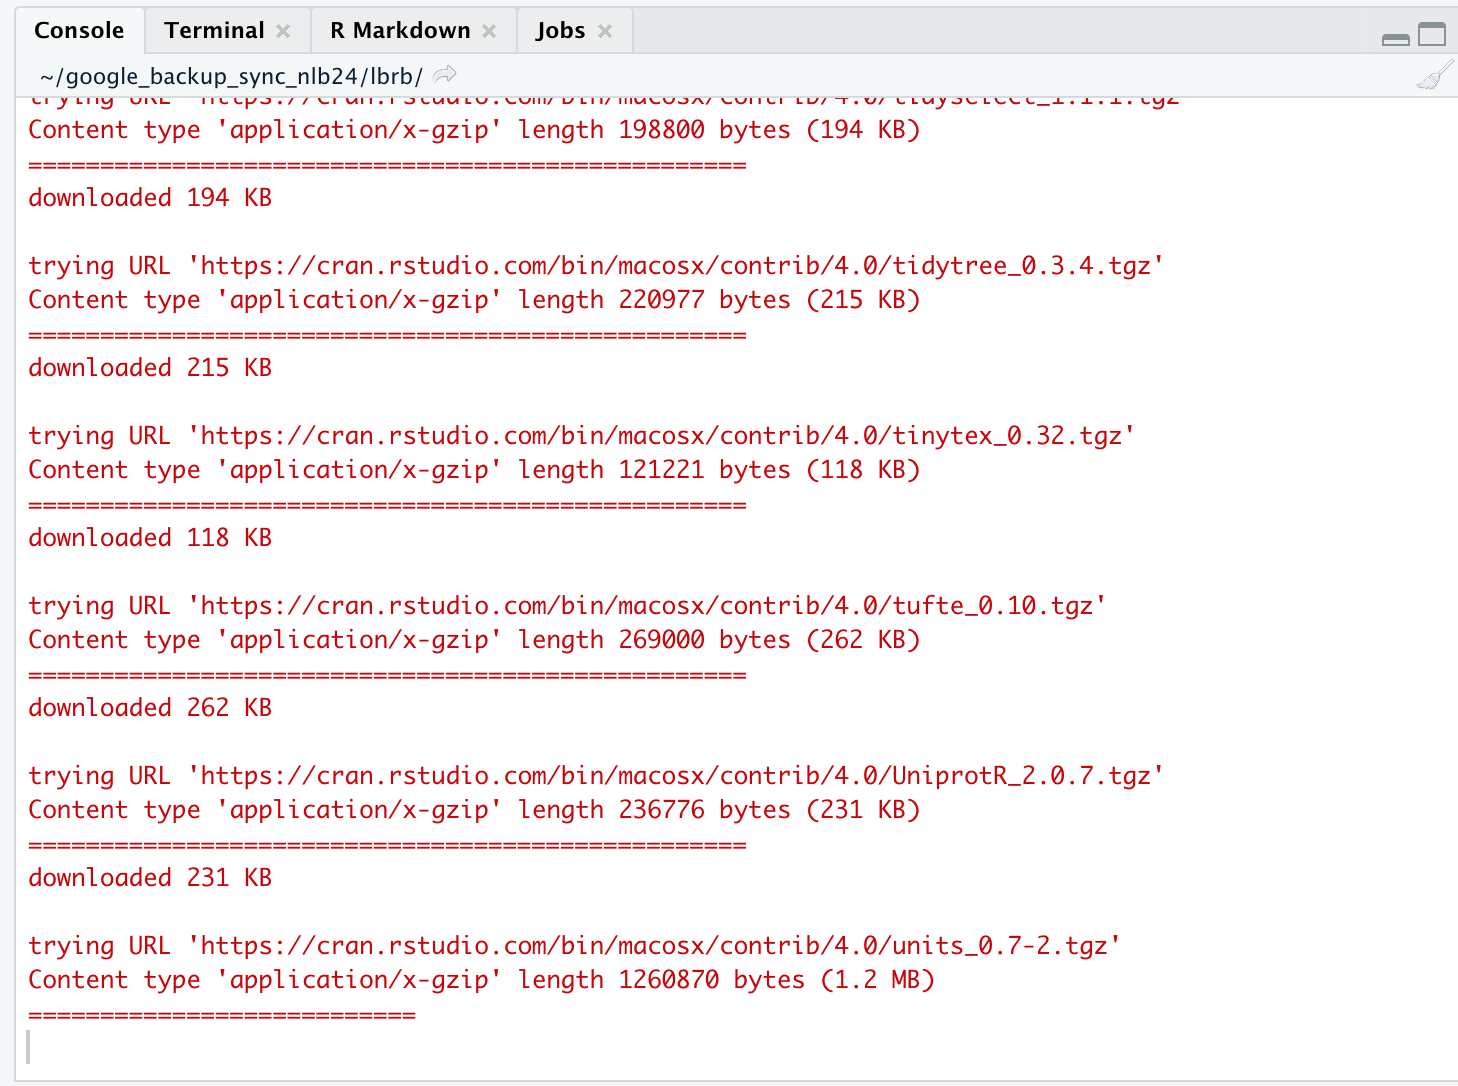
\includegraphics[width=0.4\linewidth]{images/angry_red_text_download_biostrings}

\hypertarget{actually-loading-a-package}{%
\section{Actually loading a package}\label{actually-loading-a-package}}

Again, to actually load the \passthrough{\lstinline!Biostrings!} package into your active R sessions requires the \passthrough{\lstinline!libary()!} command:

\begin{lstlisting}[language=R]
library(Biostrings)
\end{lstlisting}

As you might expect, there's more red text scrolling up my screen!

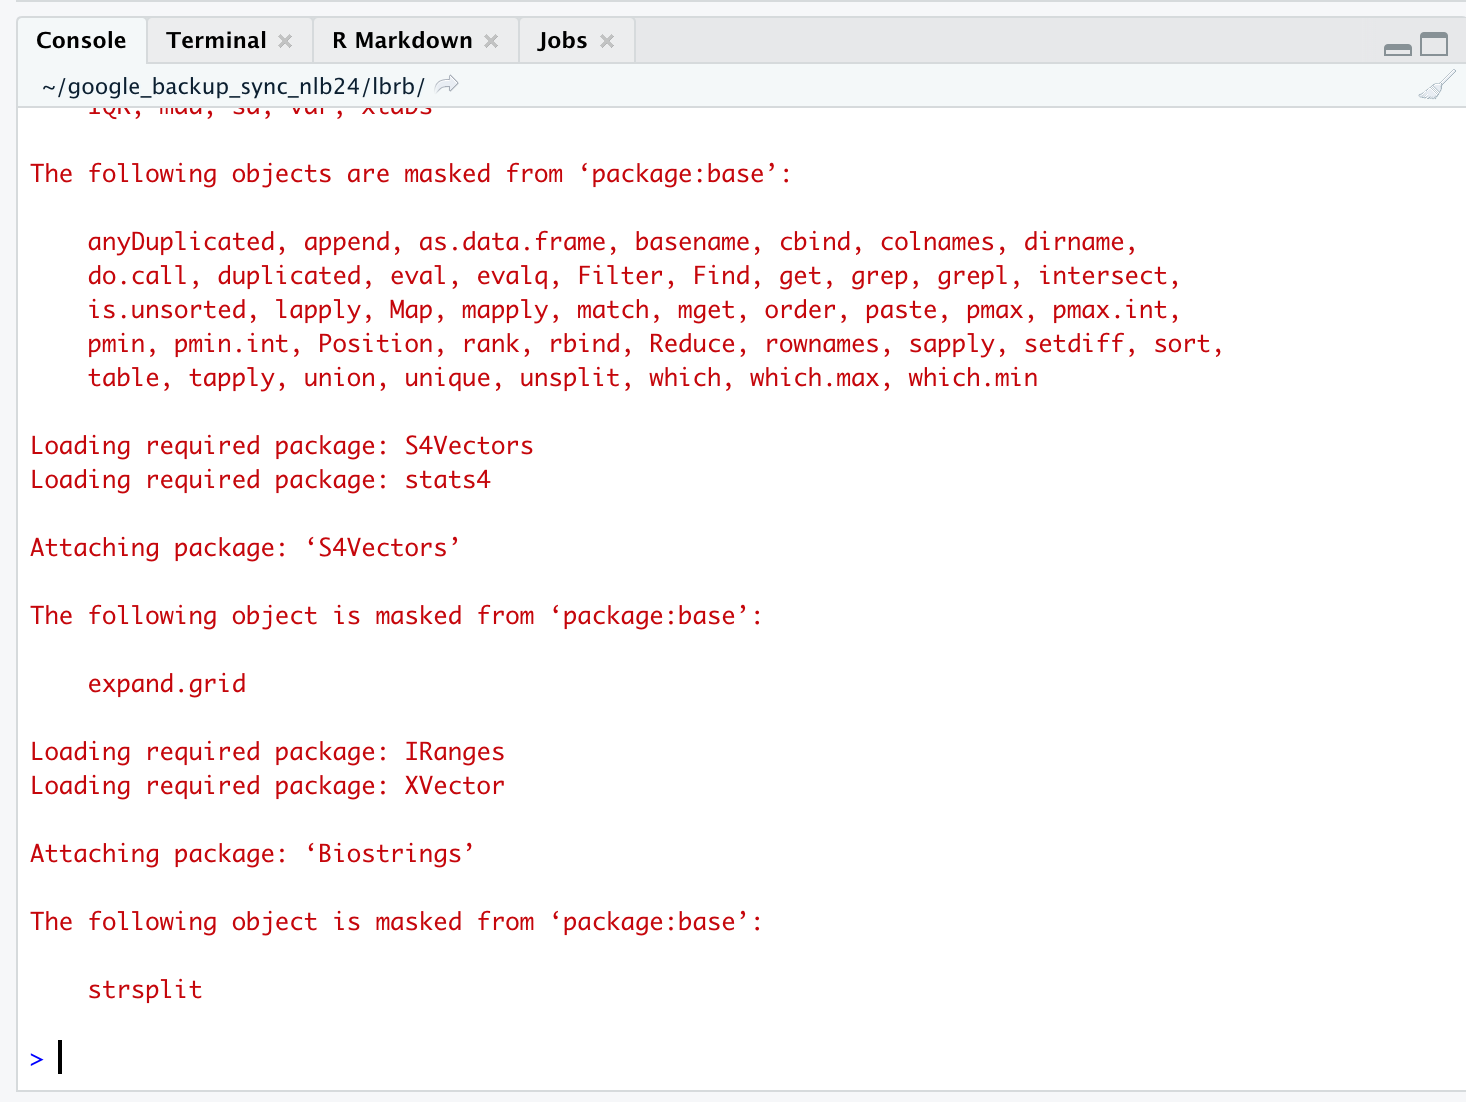
\includegraphics[width=0.4\linewidth]{images/angry_red_text_library_biostrings}

I can tell that is actually worked because at the end of all the red stuff is the R prompt of ``\textgreater{}'' and my cursor.


\includegraphics[width=1.42in]{images/R_cursor}

\hypertarget{basic-R}{%
\chapter{A Brief introduction to R}\label{basic-R}}

\textbf{By}: Avril Coghlan.

\textbf{Adapted, edited and expanded}: Nathan Brouwer under the Creative Commons 3.0 Attribution License \href{https://creativecommons.org/licenses/by/3.0/}{(CC BY 3.0)}.

This chapter provides a brief introduction to R. At the end of are links to additional resources for getting started with R.

\hypertarget{vocabulary}{%
\section{Vocabulary}\label{vocabulary}}

\begin{itemize}
\tightlist
\item
  scalar
\item
  vector
\item
  list
\item
  class
\item
  numeric
\item
  character
\item
  assignment
\item
  elements of an object
\item
  indices
\item
  attributes of an object
\item
  argument of a function
\end{itemize}

\hypertarget{r-functions}{%
\section{R functions}\label{r-functions}}

\begin{itemize}
\tightlist
\item
  \textless-
\item
  {[} {]}
\item
  \$
\item
  table()
\item
  function
\item
  c()
\item
  log10()
\item
  help(), ?
\item
  help.search()
\item
  RSiteSearch()
\item
  mean()
\item
  return()
\item
  q()
\end{itemize}

\hypertarget{interacting-with-r}{%
\section{Interacting with R}\label{interacting-with-r}}

You will type \emph{R} commands into the RStudio \textbf{console} in order to carry out analyses in \emph{R}. In the RStudio console you will see the R prompt starting with the symbol ``\textgreater{}''. ``\textgreater{}'' will always be there at the beginning of each new command - don't try to delete it! Moreover, you never need to type it.


\includegraphics[width=1.42in]{images/R_cursor}

We type the \textbf{commands} needed for a particular task after this prompt. The command is carried out by \emph{R} after you hit the Return key.

Once you have started R, you can start typing commands into the RStudio console, and the results will be calculated immediately, for example:

\begin{lstlisting}[language=R]
2*3
\end{lstlisting}

\begin{lstlisting}
## [1] 6
\end{lstlisting}

Note that prior to the output of ``6'' it shows ``{[}1{]}''.

Now subtraction:

\begin{lstlisting}[language=R]
10-3
\end{lstlisting}

\begin{lstlisting}
## [1] 7
\end{lstlisting}

Again, prior to the output of ``7'' it shows ``{[}1{]}''.

\emph{R} can act like a basic calculator that you type commands in to. You can also use it like a more advanced scientific calculator and create \textbf{variables} that store information. All variables created by R are called \textbf{objects}. In R, we assign values to variables using an arrow-looking function \passthrough{\lstinline!<-!} the \textbf{assignment operator}. For example, we can \textbf{assign} the value 2*3 to the variable x using the command:

\begin{lstlisting}[language=R]
x <- 2*3
\end{lstlisting}

To view the contents of any R object, just type its name, press enter, and the contents of that R object will be displayed:

\begin{lstlisting}[language=R]
x
\end{lstlisting}

\begin{lstlisting}
## [1] 6
\end{lstlisting}

\hypertarget{variables-in-r}{%
\section{Variables in R}\label{variables-in-r}}

There are several different types of objects in R with fancy math names, including \textbf{scalars}, \textbf{vectors}, \textbf{matrices} (singular: \textbf{matrix), }arrays\textbf{, }dataframes\textbf{, }tables\textbf{, and }lists\textbf{. The }scalar** variable x above is one example of an R object. While a scalar variable such as x has just one element, a \textbf{vector} consists of several elements. The elements in a vector are all of the same \textbf{type} (e.g.. numbers or alphabetic characters), while \textbf{lists} may include elements such as characters as well as numeric quantities. Vectors and dataframes are the most common variables you'll use. You'll also encounter matrices often, and lists are ubiquitous in R but beginning users often don't encounter them because they remain behind the scenes.

\hypertarget{vectors}{%
\subsection{Vectors}\label{vectors}}

To create a vector, we can use the \passthrough{\lstinline!c()!} (combine) function. For example, to create a vector called \passthrough{\lstinline!myvector!} that has elements with values 8, 6, 9, 10, and 5, we type:

\begin{lstlisting}[language=R]
myvector <- c(8, 6, 9, 10, 5) # note: commas between each number!
\end{lstlisting}

To see the contents of the variable \passthrough{\lstinline!myvector!}, we can just type its name and press enter:

\begin{lstlisting}[language=R]
myvector
\end{lstlisting}

\begin{lstlisting}
## [1]  8  6  9 10  5
\end{lstlisting}

\hypertarget{vector-indexing}{%
\subsection{Vector indexing}\label{vector-indexing}}

The \passthrough{\lstinline![1]!} is the \textbf{index} of the first \textbf{element} in the vector. We can \textbf{extract} any element of the vector by typing the vector name with the index of that element given in \textbf{square brackets} \passthrough{\lstinline![...]!}.

For example, to get the value of the 4th element in the vector \passthrough{\lstinline!myvector!}, we type:

\begin{lstlisting}[language=R]
myvector[4]
\end{lstlisting}

\begin{lstlisting}
## [1] 10
\end{lstlisting}

\hypertarget{character-vectors}{%
\subsection{Character vectors}\label{character-vectors}}

Vectors can contain letters, such as those designating nucleic acids

\begin{lstlisting}[language=R]
my.seq <- c("A","T","C","G")
\end{lstlisting}

They can also contain multi-letter \textbf{strings}:

\begin{lstlisting}[language=R]
my.oligos <- c("ATCGC","TTTCGC","CCCGCG","GGGCGC")
\end{lstlisting}

\hypertarget{lists}{%
\subsection{Lists}\label{lists}}

\textbf{NOTE}: \emph{below is a discussion of lists in R. This is excellent information, but not necessary if this is your very very first time using R.}

In contrast to a vector, a \textbf{list} can contain elements of different types, for example, both numbers and letters. A list can even include other variables such as a vector. The \passthrough{\lstinline!list()!} function is used to create a list. For example, we could create a list \passthrough{\lstinline!mylist!} by typing:

\begin{lstlisting}[language=R]
mylist <- list(name="Charles Darwin", 
               wife="Emma Darwin", 
               myvector)
\end{lstlisting}

We can then print out the contents of the list \passthrough{\lstinline!mylist!} by typing its name:

\begin{lstlisting}[language=R]
mylist
\end{lstlisting}

\begin{lstlisting}
## $name
## [1] "Charles Darwin"
## 
## $wife
## [1] "Emma Darwin"
## 
## [[3]]
## [1]  8  6  9 10  5
\end{lstlisting}

The \textbf{elements} in a list are numbered, and can be referred to using \textbf{indices}. We can extract an element of a list by typing the list name with the index of the element given in double \textbf{square brackets} (in contrast to a vector, where we only use single square brackets).

We can extract the second element from \passthrough{\lstinline!mylist!} by typing:

\begin{lstlisting}[language=R]
mylist[[2]]  # note the double square brackets [[...]]
\end{lstlisting}

\begin{lstlisting}
## [1] "Emma Darwin"
\end{lstlisting}

As a baby step towards our next task, we can wrap index values as in the \passthrough{\lstinline!c()!} command like this:

\begin{lstlisting}[language=R]
mylist[[c(2)]]  # note the double square brackets [[...]]
\end{lstlisting}

\begin{lstlisting}
## [1] "Emma Darwin"
\end{lstlisting}

The number \passthrough{\lstinline!2!} and \passthrough{\lstinline!c(2)!} mean the same thing.

Now, we can extract the second AND third elements from \passthrough{\lstinline!mylist!}. First, we put the indices 2 and 3 into a vector \passthrough{\lstinline!c(2,3)!}, then wrap that vector in double square brackets: \passthrough{\lstinline![c(2,3)]!}. All together it looks like this.

\begin{lstlisting}[language=R]
mylist[c(2,3)] # note the double brackets
\end{lstlisting}

\begin{lstlisting}
## $wife
## [1] "Emma Darwin"
## 
## [[2]]
## [1]  8  6  9 10  5
\end{lstlisting}

Elements of lists may also be named, resulting in a \textbf{named lists}. The elements may then be referred to by giving the list name, followed by ``\$'', followed by the element name. For example, mylist\$name is the same as mylist{[}{[}1{]}{]} and mylist\$wife is the same as mylist{[}{[}2{]}{]}:

\begin{lstlisting}[language=R]
mylist$wife
\end{lstlisting}

\begin{lstlisting}
## [1] "Emma Darwin"
\end{lstlisting}

We can find out the names of the named elements in a list by using the \passthrough{\lstinline!attributes()!} function, for example:

\begin{lstlisting}[language=R]
attributes(mylist)
\end{lstlisting}

\begin{lstlisting}
## $names
## [1] "name" "wife" ""
\end{lstlisting}

When you use the \passthrough{\lstinline!attributes()!} function to find the named elements of a list variable, the named elements are always listed under a heading ``\$names''. Therefore, we see that the named elements of the list variable \passthrough{\lstinline!mylist!} are called ``name'' and ``wife'', and we can retrieve their values by typing mylist\$name and mylist\$wife, respectively.

\hypertarget{tables}{%
\subsection{Tables}\label{tables}}

Another type of object that you will encounter in R is a \textbf{table}. The \passthrough{\lstinline!table()!} function allows you to total up or tabulate the number of times a value occurs within a vector. Tables are typically used on vectors containing \textbf{character data}, such as letters, words, or names, but can work on numeric data data.

\hypertarget{tables---the-basics}{%
\subsubsection{Tables - The basics}\label{tables---the-basics}}

If we made a vector variable ``nucleotides'' containing the of a DNA molecule, we can use the \passthrough{\lstinline!table()!} function to produce a \textbf{table variable} that contains the number of bases with each possible nucleotides:

\begin{lstlisting}[language=R]
bases <- c("A", "T", "A", "A", "T", "C", "G", "C", "G")
\end{lstlisting}

Now make the table

\begin{lstlisting}[language=R]
table(bases)
\end{lstlisting}

\begin{lstlisting}
## bases
## A C G T 
## 3 2 2 2
\end{lstlisting}

We can store the table variable produced by the function \passthrough{\lstinline!table()!}, and call the stored table ``bases.table'', by typing:

\begin{lstlisting}[language=R]
bases.table <- table(bases)
\end{lstlisting}

Tables also work on vectors containing numbers. First, a vector of numbers.

\begin{lstlisting}[language=R]
numeric.vecter <- c(1,1,1,1,3,4,4,4,4)
\end{lstlisting}

Second, a table, showing how many times each number occurs.

\begin{lstlisting}[language=R]
table(numeric.vecter)
\end{lstlisting}

\begin{lstlisting}
## numeric.vecter
## 1 3 4 
## 4 1 4
\end{lstlisting}

\hypertarget{tables---further-details}{%
\subsubsection{Tables - further details}\label{tables---further-details}}

To access elements in a table variable, you need to use double square brackets, just like accessing elements in a list. For example, to access the fourth element in the table bases.table (the number of Ts in the sequence), we type:

\begin{lstlisting}[language=R]
bases.table[[4]]  # double brackets!
\end{lstlisting}

\begin{lstlisting}
## [1] 2
\end{lstlisting}

Alternatively, you can use the name of the fourth element in the table (``John'') to find the value of that table element:

\begin{lstlisting}[language=R]
bases.table[["T"]]
\end{lstlisting}

\begin{lstlisting}
## [1] 2
\end{lstlisting}

\hypertarget{arguments}{%
\section{Arguments}\label{arguments}}

Functions in R usually require \textbf{arguments}, which are input variables (i.e.. objects) that are \textbf{passed} to them, which they then carry out some operation on. For example, the \passthrough{\lstinline!log10()!} function is passed a number, and it then calculates the log to the base 10 of that number:

\begin{lstlisting}[language=R]
log10(100)
\end{lstlisting}

\begin{lstlisting}
## [1] 2
\end{lstlisting}

There's a more generic function, \passthrough{\lstinline!log()!}, where we pass it not only a number to take the log of, but also the specific \textbf{base} of the logarithm. To take the log base 10 with the \passthrough{\lstinline!log()!} function we do this

\begin{lstlisting}[language=R]
log(100, base = 10)
\end{lstlisting}

\begin{lstlisting}
## [1] 2
\end{lstlisting}

We can also take logs with other bases, such as 2:

\begin{lstlisting}[language=R]
log(100, base = 2)
\end{lstlisting}

\begin{lstlisting}
## [1] 6.643856
\end{lstlisting}

\hypertarget{help-files-with-help-and}{%
\section{\texorpdfstring{Help files with \texttt{help()} and \texttt{?}}{Help files with help() and ?}}\label{help-files-with-help-and}}

In \emph{R}, you can get help about a particular function by using the \passthrough{\lstinline!help()!} function. For example, if you want help about the \passthrough{\lstinline!log10()!} function, you can type:

\begin{lstlisting}[language=R]
help("log10")
\end{lstlisting}

When you use the \passthrough{\lstinline!help()!} function, a box or web page will show up in one of the panes of RStudio with information about the function that you asked for help with. You can also use the \passthrough{\lstinline!?!} next to the function like this

\begin{lstlisting}[language=R]
?log10
\end{lstlisting}

Help files are a mixed bag in R, and it can take some getting used to them. An excellent overview of this is Kieran Healy's \href{https://socviz.co/appendix.html}{``How to read an R help page.''}

\hypertarget{searching-for-functions-with-help.search-and-rsitesearch}{%
\section{\texorpdfstring{Searching for functions with \texttt{help.search()} and \texttt{RSiteSearch()}}{Searching for functions with help.search() and RSiteSearch()}}\label{searching-for-functions-with-help.search-and-rsitesearch}}

If you are not sure of the name of a function, but think you know part of its name, you can search for the function name using the \passthrough{\lstinline!help.search()!} and \passthrough{\lstinline!RSiteSearch()!} functions. The \passthrough{\lstinline!help.search()!} function searches to see if you already have a function installed (from one of the R packages that you have installed) that may be related to some topic you're interested in. \passthrough{\lstinline!RSiteSearch()!} searches \emph{all} R functions (including those in packages that you haven't yet installed) for functions related to the topic you are interested in.

For example, if you want to know if there is a function to calculate the standard deviation (SD) of a set of numbers, you can search for the names of all installed functions containing the word ``deviation'' in their description by typing:

\begin{lstlisting}[language=R]
help.search("deviation")
\end{lstlisting}

Among the functions that were found, is the function \passthrough{\lstinline!sd()!} in the \passthrough{\lstinline!stats!} package (an R package that comes with the base R installation), which is used for calculating the standard deviation.

Now, instead of searching just the packages we've have on our computer let's search all R packages on CRAN. Let's look for things related to DNA. Note that \passthrough{\lstinline!RSiteSearch()!} doesn't provide output within RStudio, but rather opens up your web browser for you to display the results.

\begin{lstlisting}[language=R]
RSiteSearch("DNA")
\end{lstlisting}

The results of the \passthrough{\lstinline!RSiteSearch()!} function will be hits to descriptions of R functions, as well as to R mailing list discussions of those functions.

\hypertarget{more-on-functions}{%
\section{More on functions}\label{more-on-functions}}

We can perform computations with R using objects such as scalars and vectors. For example, to calculate the average of the values in the vector \passthrough{\lstinline!myvector!} (i.e.. the average of 8, 6, 9, 10 and 5), we can use the \passthrough{\lstinline!mean()!} function:

\begin{lstlisting}[language=R]
mean(myvector) # note: no " "
\end{lstlisting}

\begin{lstlisting}
## [1] 7.6
\end{lstlisting}

We have been using built-in R functions such as mean(), length(), print(), plot(), etc.

\hypertarget{writing-your-own-functions}{%
\subsection{Writing your own functions}\label{writing-your-own-functions}}

\textbf{NOTE}: *Writing your own functions is an advanced skills. New users can skip this section.

We can also create our own functions in R to do calculations that you want to carry out very often on different input data sets. For example, we can create a function to calculate the value of 20 plus square of some input number:

\begin{lstlisting}[language=R]
myfunction <- function(x) { return(20 + (x*x)) }
\end{lstlisting}

This function will calculate the square of a number (x), and then add 20 to that value. The \passthrough{\lstinline!return()!} statement returns the calculated value. Once you have typed in this function, the function is then available for use. For example, we can use the function for different input numbers (e.g.. 10, 25):

\begin{lstlisting}[language=R]
myfunction(10)
\end{lstlisting}

\begin{lstlisting}
## [1] 120
\end{lstlisting}

\hypertarget{quiting-r}{%
\section{Quiting R}\label{quiting-r}}

To quit R either close the program, or type:

\begin{lstlisting}[language=R]
q()
\end{lstlisting}

\hypertarget{links-and-further-reading}{%
\section{Links and Further Reading}\label{links-and-further-reading}}

Some links are included here for further reading.

For a more in-depth introduction to R, a good online tutorial is available on the ``Kickstarting R'' website, cran.r-project.org/doc/contrib/Lemon-kickstart.

There is another nice (slightly more in-depth) tutorial to R available on the ``Introduction to R'' website, cran.r-project.org/doc/manuals/R-intro.html.

\href{https://learningstatisticswithr.com/book/introR.html}{Chapter 3} of Danielle Navarro's book is an excellent intro to the basics of R.

\hypertarget{vectors-in-R}{%
\chapter{A primer for working with vectors}\label{vectors-in-R}}

\textbf{By}: Avril Coghlan

\textbf{Adapted, edited and expanded}: Nathan Brouwer (\href{mailto:brouwern@gmail.com}{\nolinkurl{brouwern@gmail.com}}) under the Creative Commons 3.0 Attribution License \href{https://creativecommons.org/licenses/by/3.0/}{(CC BY 3.0)}.

\hypertarget{preface-1}{%
\section{Preface}\label{preface-1}}

This is a modification of part of\href{https://a-little-book-of-r-for-bioinformatics.readthedocs.io/en/latest/src/chapter2.html}{``DNA Sequence Statistics (2)''} from Avril Coghlan's \href{https://a-little-book-of-r-for-bioinformatics.readthedocs.io/en/latest/index.html}{\emph{A little book of R for bioinformatics.}}. Most of text and code was originally written by Dr.~Coghlan and distributed under the \href{https://creativecommons.org/licenses/by/3.0/us/}{Creative Commons 3.0} license.

\hypertarget{vocab}{%
\section{Vocab}\label{vocab}}

\begin{itemize}
\tightlist
\item
  base R
\item
  scalar, vector, matrix
\item
  vectorized operation
\item
  regular expressions
\end{itemize}

\hypertarget{functions}{%
\chapter{Functions}\label{functions}}

\begin{itemize}
\tightlist
\item
  \passthrough{\lstinline!seq()!}
\item
  \passthrough{\lstinline!is()!}, \passthrough{\lstinline!is.vector()!}, \passthrough{\lstinline!is.matrix()!}
\item
  \passthrough{\lstinline!gsub()!}
\end{itemize}

\hypertarget{vectors-in-r}{%
\section{Vectors in R}\label{vectors-in-r}}

\textbf{Variables} in R include \textbf{scalars}, \textbf{vectors}, and \textbf{lists}. \textbf{Functions} in R carry out operations on variables, for example, using the \passthrough{\lstinline!log10()!} function to calculate the log to the base 10 of a scalar variable \passthrough{\lstinline!x!}, or using the \passthrough{\lstinline!mean()!} function to calculate the average of the values in a vector variable \passthrough{\lstinline!myvector!}. For example, we can use \passthrough{\lstinline!log10()!} on a scalar object like this:

\begin{lstlisting}[language=R]
# store value in object
x <- 100

# take log base 10 of object
log10(x)
\end{lstlisting}

\begin{lstlisting}
## [1] 2
\end{lstlisting}

Note that while mathematically x is a single number, or a scalar, R considers it to be a vector:

\begin{lstlisting}[language=R]
is.vector(x)
\end{lstlisting}

\begin{lstlisting}
## [1] TRUE
\end{lstlisting}

There are many ``is'' commands. What is returned when you run \passthrough{\lstinline!is.matrix()!} on a vector?

\begin{lstlisting}[language=R]
is.matrix(x)
\end{lstlisting}

\begin{lstlisting}
## [1] FALSE
\end{lstlisting}

Mathematically this is a bit odd, since often a vector is defined as a one-dimensional matrix, e.g., a single column or single row of a matrix. But in \emph{R} land, a vector is a vector, and matrix is a matrix, and there are no explicit scalars.

\hypertarget{math-on-vectors}{%
\section{Math on vectors}\label{math-on-vectors}}

Vectors can serve as the input for mathematical operations. When this is done \emph{R} does the mathematical operation separately on each element of the vector. This is a unique feature of \emph{R} that can be hard to get used to even for people with previous programming experience.

Let's make a vector of numbers:

\begin{lstlisting}[language=R]
myvector <- c(30,16,303,99,11,111)
\end{lstlisting}

What happens when we multiply \passthrough{\lstinline!myvector!} by 10?

\begin{lstlisting}[language=R]
myvector*10
\end{lstlisting}

\begin{lstlisting}
## [1]  300  160 3030  990  110 1110
\end{lstlisting}

R has taken each of the 6 values, 30 through 111, of \passthrough{\lstinline!myvector!} and multiplied each one by 10, giving us 6 results. That is, what R did was

\begin{lstlisting}[language=R]
## 30*10    # first value of myvector
## 16*10    # second value of myvector
## 303*10   # ....
## 99*10
## 111*10   # last value of myvector
\end{lstlisting}

The normal order of operations rules apply to vectors as they do to operations we're more used to. So multiplying \passthrough{\lstinline!myvector!} by 10 is the same whether you put he 10 before or after vector. That is \passthrough{\lstinline!myvector\\*10!} is the same as \passthrough{\lstinline!10\\*myvector!}.

\begin{lstlisting}[language=R]
myvector*10
\end{lstlisting}

\begin{lstlisting}
## [1]  300  160 3030  990  110 1110
\end{lstlisting}

\begin{lstlisting}[language=R]
10*myvector
\end{lstlisting}

\begin{lstlisting}
## [1]  300  160 3030  990  110 1110
\end{lstlisting}

What happen when you subtract 30 from myvector? Write the code below.

\begin{lstlisting}[language=R]
myvector-30
\end{lstlisting}

\begin{lstlisting}
## [1]   0 -14 273  69 -19  81
\end{lstlisting}

So, what R did was

\begin{lstlisting}[language=R]
## 30-30    # first value of myvector
## 16-30    # second value of myvector
## 303-30   # ....
## 99-30
## 111-30   # last value of myvector
\end{lstlisting}

Again, \passthrough{\lstinline!myvector-30!} is vectorized operation.

You can also square a vector

\begin{lstlisting}[language=R]
myvector^2
\end{lstlisting}

\begin{lstlisting}
## [1]   900   256 91809  9801   121 12321
\end{lstlisting}

Which is the same as

\begin{lstlisting}[language=R]
## 30^2    # first value of myvector
## 16^2    # second value of myvector
## 303^2   # ....
## 99^2
## 111^2   # last value of myvector
\end{lstlisting}

Also you can take the square root of a vector using the functions \passthrough{\lstinline!sqrt()!}\ldots{}

\begin{lstlisting}[language=R]
sqrt(myvector)
\end{lstlisting}

\begin{lstlisting}
## [1]  5.477226  4.000000 17.406895  9.949874  3.316625 10.535654
\end{lstlisting}

\ldots and take the log of a vector with \passthrough{\lstinline!log()!}\ldots{}

\begin{lstlisting}[language=R]
log(myvector)
\end{lstlisting}

\begin{lstlisting}
## [1] 3.401197 2.772589 5.713733 4.595120 2.397895 4.709530
\end{lstlisting}

\ldots and just about any other mathematical operation. Here we are working on a separate vector object; all of these rules apply to a column in a matrix or a dataframe.

This attribute of R is called \textbf{vectorization}. When you run the code \passthrough{\lstinline!myvector*10!} or \passthrough{\lstinline!log(myvector)!} you are doing a \textbf{vectorized} operation - its like normal math with special vector-based super power to get more done faster than you normally could.

\hypertarget{functions-on-vectors}{%
\section{Functions on vectors}\label{functions-on-vectors}}

As we just saw, we can use functions on vectors. Typically these use the vectors as an input and all the numbers are processed into an output. Call the \passthrough{\lstinline!mean()!} function on the vector we made called \passthrough{\lstinline!myvector!}.

\begin{lstlisting}[language=R]
mean(myvector)
\end{lstlisting}

\begin{lstlisting}
## [1] 95
\end{lstlisting}

Note how we get a single value back - the mean of all the values in the vector. R saw that we had a vector of multiple and knew that the mean is a function that doesn't get applied to single number, but sets of numbers.

The function \passthrough{\lstinline!sd()!} calculates the standard deviation. Apply the \passthrough{\lstinline!sd()!} to myvector:

\begin{lstlisting}[language=R]
sd(myvector)
\end{lstlisting}

\begin{lstlisting}
## [1] 110.5061
\end{lstlisting}

\hypertarget{operations-with-two-vectors}{%
\section{Operations with two vectors}\label{operations-with-two-vectors}}

You can also subtract one vector from another vector. This can be a little weird when you first see it. Make another vector with the numbers 5, 10, 15, 20, 25, 30. Call this myvector2:

\begin{lstlisting}[language=R]
myvector2 <- c(5, 10, 15, 20, 25, 30)
\end{lstlisting}

Now subtract myvector2 from myvector. What happens?

\begin{lstlisting}[language=R]
myvector-myvector2
\end{lstlisting}

\begin{lstlisting}
## [1]  25   6 288  79 -14  81
\end{lstlisting}

\hypertarget{subsetting-vectors}{%
\section{Subsetting vectors}\label{subsetting-vectors}}

You can extract an \textbf{element} of a vector by typing the vector name with the index of that element given in \textbf{square brackets}. For example, to get the value of the 3rd element in the vector \passthrough{\lstinline!myvector!}, we type:

\begin{lstlisting}[language=R]
myvector[3]
\end{lstlisting}

\begin{lstlisting}
## [1] 303
\end{lstlisting}

Extract the 4th element of the vector:

\begin{lstlisting}[language=R]
myvector[4]
\end{lstlisting}

\begin{lstlisting}
## [1] 99
\end{lstlisting}

You can extract more than one element by using a vector in the brackets:

First, say I want to extract the 3rd and the 4th element. I can make a vector with 3 and 4 in it:

\begin{lstlisting}[language=R]
nums <- c(3,4)
\end{lstlisting}

Then put that vector in the brackets:

\begin{lstlisting}[language=R]
myvector[nums]
\end{lstlisting}

\begin{lstlisting}
## [1] 303  99
\end{lstlisting}

We can also do it directly like this, skipping the vector-creation step:

\begin{lstlisting}[language=R]
myvector[c(3,4)]
\end{lstlisting}

\begin{lstlisting}
## [1] 303  99
\end{lstlisting}

In the chunk below extract the 1st and 2nd elements:

\begin{lstlisting}[language=R]
myvector[c(1,2)]
\end{lstlisting}

\begin{lstlisting}
## [1] 30 16
\end{lstlisting}

\hypertarget{sequences-of-numbers}{%
\section{Sequences of numbers}\label{sequences-of-numbers}}

Often we want a vector of numbers in \textbf{sequential order}. That is, a vector with the numbers 1, 2, 3, 4, \ldots{} or 5, 10, 15, 20, \ldots{} The easiest way to do this is using a colon

\begin{lstlisting}[language=R]
1:10
\end{lstlisting}

\begin{lstlisting}
##  [1]  1  2  3  4  5  6  7  8  9 10
\end{lstlisting}

Note that in R 1:10 is equivalent to c(1:10)

\begin{lstlisting}[language=R]
c(1:10)
\end{lstlisting}

\begin{lstlisting}
##  [1]  1  2  3  4  5  6  7  8  9 10
\end{lstlisting}

Usually to emphasize that a vector is being created I will use c(1:10)

We can do any number to any numbers

\begin{lstlisting}[language=R]
c(20:30)
\end{lstlisting}

\begin{lstlisting}
##  [1] 20 21 22 23 24 25 26 27 28 29 30
\end{lstlisting}

We can also do it in \emph{reverse}. In the code below put 30 before 20:

\begin{lstlisting}[language=R]
c(30:20)
\end{lstlisting}

\begin{lstlisting}
##  [1] 30 29 28 27 26 25 24 23 22 21 20
\end{lstlisting}

A useful function in \emph{R} is the \passthrough{\lstinline!seq()!} function, which is an explicit function that can be used to create a vector containing a sequence of numbers that run from a particular number to another particular number.

\begin{lstlisting}[language=R]
seq(1, 10)
\end{lstlisting}

\begin{lstlisting}
##  [1]  1  2  3  4  5  6  7  8  9 10
\end{lstlisting}

Using \passthrough{\lstinline!seq()!} instead of a \passthrough{\lstinline!:!} can be useful for readability to make it explicit what is going on. More importantly, \passthrough{\lstinline!seq!} has an argument \passthrough{\lstinline!by = ...!} so you can make a sequence of number with any interval between For example, if we want to create the sequence of numbers from 1 to 10 in steps of 1 (i.e.. 1, 2, 3, 4, \ldots{} 10), we can type:

\begin{lstlisting}[language=R]
seq(1, 10,
    by = 1)
\end{lstlisting}

\begin{lstlisting}
##  [1]  1  2  3  4  5  6  7  8  9 10
\end{lstlisting}

We can change the \textbf{step size} by altering the value of the \passthrough{\lstinline!by!} argument given to the function \passthrough{\lstinline!seq()!}. For example, if we want to create a sequence of numbers from 1-100 in steps of 20 (i.e.. 1, 21, 41, \ldots{} 101), we can type:

\begin{lstlisting}[language=R]
seq(1, 101,
    by = 20)
\end{lstlisting}

\begin{lstlisting}
## [1]   1  21  41  61  81 101
\end{lstlisting}

\hypertarget{vectors-can-hold-numeric-or-character-data}{%
\section{Vectors can hold numeric or character data}\label{vectors-can-hold-numeric-or-character-data}}

The vector we created above holds numeric data, as indicated by \passthrough{\lstinline!class()!}

\begin{lstlisting}[language=R]
class(myvector)
\end{lstlisting}

\begin{lstlisting}
## [1] "numeric"
\end{lstlisting}

Vectors can also holder character data, like the genetic code:

\begin{lstlisting}[language=R]
# vector of character data
myvector <- c("A","T","G")

# how it looks
myvector
\end{lstlisting}

\begin{lstlisting}
## [1] "A" "T" "G"
\end{lstlisting}

\begin{lstlisting}[language=R]
# what is "is"
class(myvector)
\end{lstlisting}

\begin{lstlisting}
## [1] "character"
\end{lstlisting}

\hypertarget{regular-expressions-can-modify-character-data}{%
\section{Regular expressions can modify character data}\label{regular-expressions-can-modify-character-data}}

We can use \textbf{regular expressions} to modify character data. For example, change the Ts to Us

\begin{lstlisting}[language=R]
myvector <- gsub("T", "U", myvector)
\end{lstlisting}

Now check it out

\begin{lstlisting}[language=R]
myvector
\end{lstlisting}

\begin{lstlisting}
## [1] "A" "U" "G"
\end{lstlisting}

Regular expressions are a deep subject in computing. You can find some more information about them \href{https://rstudio-pubs-static.s3.amazonaws.com/74603_76cd14d5983f47408fdf0b323550b846.html}{here}.

\hypertarget{plotting-vectors}{%
\chapter{Plotting vectors in base R}\label{plotting-vectors}}

\textbf{By}: Avril Coghlan

\textbf{Adapted, edited and expanded}: Nathan Brouwer (\href{mailto:brouwern@gmail.com}{\nolinkurl{brouwern@gmail.com}}) under the Creative Commons 3.0 Attribution License \href{https://creativecommons.org/licenses/by/3.0/}{(CC BY 3.0)}.

\hypertarget{preface-2}{%
\section{Preface}\label{preface-2}}

This is a modification of part of\href{https://a-little-book-of-r-for-bioinformatics.readthedocs.io/en/latest/src/chapter2.html}{``DNA Sequence Statistics (2)''} from Avril Coghlan's \href{https://a-little-book-of-r-for-bioinformatics.readthedocs.io/en/latest/index.html}{\emph{A little book of R for bioinformatics.}}. Most of text and code was originally written by Dr.~Coghlan and distributed under the \href{https://creativecommons.org/licenses/by/3.0/us/}{Creative Commons 3.0} license.

\hypertarget{plotting-numeric-data}{%
\section{Plotting numeric data}\label{plotting-numeric-data}}

R allows the production of a variety of plots, including \textbf{scatterplots}, \textbf{histograms}, \textbf{piecharts}, and \textbf{boxplots}. Usually we make plots from \textbf{dataframes} with 2 or more columns, but we can also make them from two separate vectors. This flexibility is useful, but also can cause some confusion.

For example, if you have two equal-length vectors of numbers \passthrough{\lstinline!numeric.vect1!} and \passthrough{\lstinline!numeric.vect1!}, you can plot a \href{https://en.wikipedia.org/wiki/Scatter_plot}{\textbf{scatterplot}} of the values in \passthrough{\lstinline!myvector1!} against the values in \passthrough{\lstinline!myvector2!} using the \textbf{base R} \passthrough{\lstinline!plot()!}function.

First, let's make up some data in put it in vectors:

\begin{lstlisting}[language=R]
numeric.vect1 <- c(10, 15,  22,  35,  43)
numeric.vect2 <- c(3,  3.2, 3.9, 4.1, 5.2)
\end{lstlisting}

Not plot with the base R \passthrough{\lstinline!plot()!} function:

\begin{lstlisting}[language=R]
plot(numeric.vect1, numeric.vect2)
\end{lstlisting}

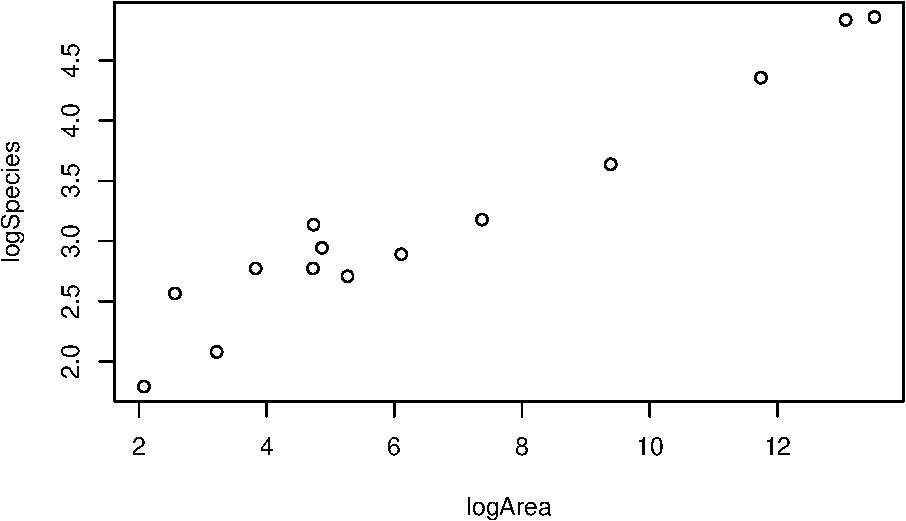
\includegraphics{lbrb_files/figure-latex/unnamed-chunk-84-1.pdf}

Note that there is a comma between the two vector names. When building plots from dataframes you usually see a tilde (\textasciitilde), but when you have two vectors you can use just a comma.

Also note the order of the vectors within the \passthrough{\lstinline!plot()!} command and which axes they appear on. The first vector is \passthrough{\lstinline!numeric.vect1!} and it appears on the horizontal x-axis.

If you want to label the axes on the plot, you can do this by giving the \passthrough{\lstinline!plot()!} function values for its optional arguments \passthrough{\lstinline!xlab =!} and \passthrough{\lstinline!ylab =!}:

\begin{lstlisting}[language=R]
plot(numeric.vect1,   # note again the comma, not a ~
     numeric.vect2, 
     xlab="vector1", 
     ylab="vector2")
\end{lstlisting}

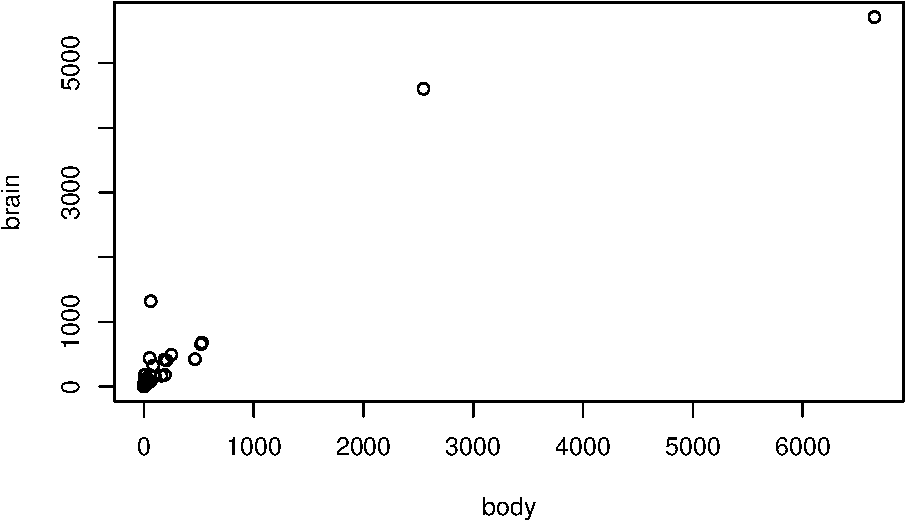
\includegraphics{lbrb_files/figure-latex/unnamed-chunk-85-1.pdf}

We can store character data in vectors so if we want we could do this to set up our labels:

\begin{lstlisting}[language=R]
mylabels <-  c("numeric.vect1","numeric.vect2")
\end{lstlisting}

Then use bracket notation to call the labels from the vector

\begin{lstlisting}[language=R]
plot(numeric.vect1, 
     numeric.vect2, 
     xlab=mylabels[1],
     ylab=mylabels[2])
\end{lstlisting}

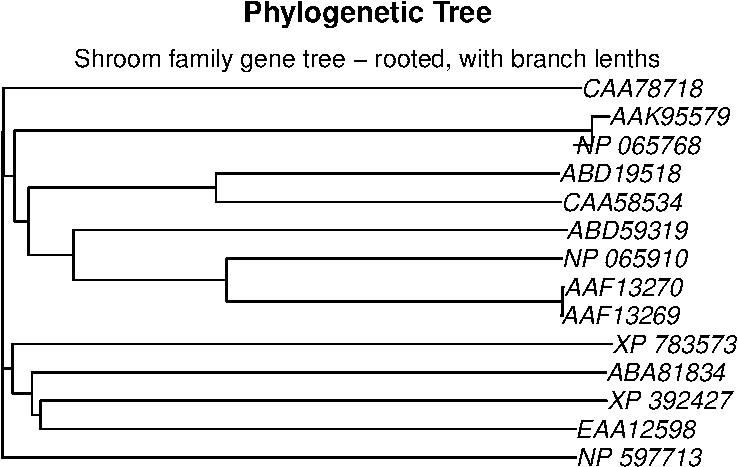
\includegraphics{lbrb_files/figure-latex/unnamed-chunk-87-1.pdf}

If we want we can use a tilde to make our plot like this:

\begin{lstlisting}[language=R]
plot(numeric.vect2 ~ numeric.vect1)
\end{lstlisting}

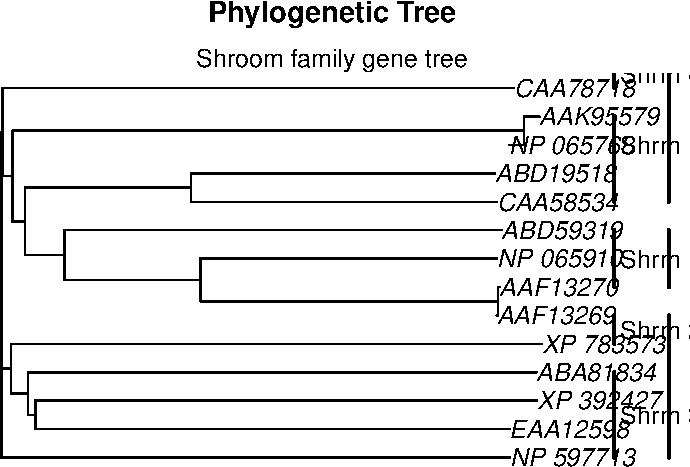
\includegraphics{lbrb_files/figure-latex/unnamed-chunk-88-1.pdf}

Note that now, \passthrough{\lstinline!numeric.vect2!} is on the left and \passthrough{\lstinline!numeric.vect1!} is on the right. This flexibility can be tricky to keep track of.

We can also combine these vectors into a dataframe and plot the data by referencing the data frame. First, we combine the two separate vectors into a dataframe using the \passthrough{\lstinline!cbind()!} command.

\begin{lstlisting}[language=R]
df <- cbind(numeric.vect1, numeric.vect2)
\end{lstlisting}

Then we plot it like this, referencing the dataframe \passthrough{\lstinline!df!} via the \passthrough{\lstinline!data = ...!} argument.

\begin{lstlisting}[language=R]
plot(numeric.vect2 ~ numeric.vect1, data = df)
\end{lstlisting}

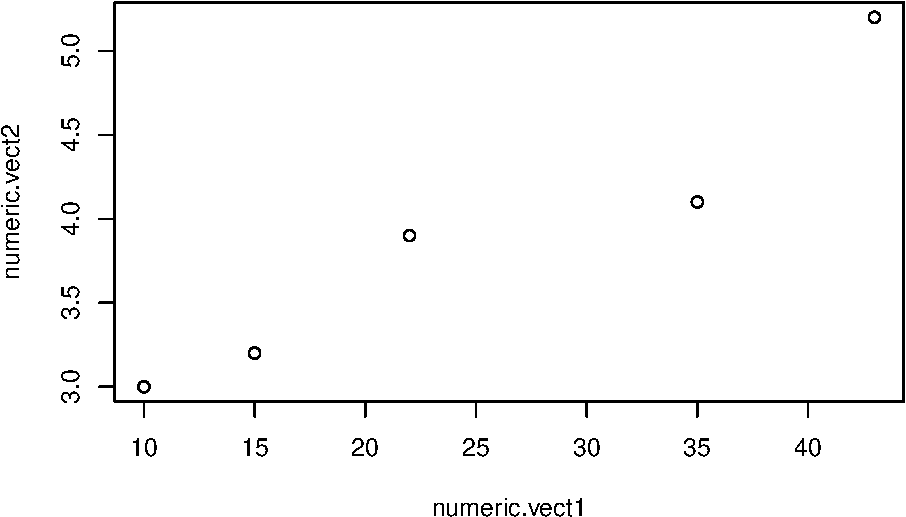
\includegraphics{lbrb_files/figure-latex/unnamed-chunk-90-1.pdf}

\hypertarget{other-plotting-packages}{%
\section{Other plotting packages}\label{other-plotting-packages}}

Base R has lots of plotting functions; additionally, people have written packages to implement new plotting capabilities. The package \passthrough{\lstinline!ggplot2!} is currently the most popular plotting package, and \passthrough{\lstinline!ggpubr!} is a package which makes \passthrough{\lstinline!ggplot2!} easier to use. For quick plots we'll use base R functions, and when we get to more important things we'll use ggplot2 and ggpubr.

\hypertarget{R-objects}{%
\chapter{Intro to R objects}\label{R-objects}}

\textbf{By}: Nathan Brouwer

\hypertarget{commands-used}{%
\section{Commands used}\label{commands-used}}

\begin{itemize}
\tightlist
\item
  \textless-
\item
  c()
\item
  length()
\item
  dim()
\item
  is()
\end{itemize}

\hypertarget{r-objects}{%
\section{R Objects}\label{r-objects}}

\begin{itemize}
\tightlist
\item
  Everything in R is an object, works with an object, tells you about an object, etc
\item
  We'll do a simple data analysis with a t.test and then look at properties of R objects
\item
  There are several types of objects: \textbf{vectors, matrices, lists, dataframes}
\item
  R objects can hold numbers, text, or both
\item
  A typical dataframe has columns of \textbf{numeric data} and columns of text that represent \textbf{factor variables} (aka ``\textbf{categorical variables}'')
\end{itemize}

\hypertarget{differences-between-objects}{%
\section{Differences between objects}\label{differences-between-objects}}

Different objects are used and show up in different contexts.

\begin{itemize}
\tightlist
\item
  Most practical stats work in R is done with \textbf{dataframes} .\\
\item
  A dataframe is kind of like a spreadsheet, loaded into R.
\item
  For the sake of simplicity, we often load data in as a \textbf{vector}. This just makes things smoother when we are starting out.
\item
  \textbf{vectors} pop up in many places, usually in a support role until you start doing more programming.
\item
  \textbf{matrices} are occasionally used for applied stats stuff but show up more for programming. A matrix is like a stripped-down dataframe.
\item
  \textbf{lists} show up everywhere, but you often don't know it; many R functions make lists
\item
  Understanding \textbf{lists} will help you efficiently work with stats output and make plots.
\end{itemize}

\hypertarget{the-data}{%
\section{The Data}\label{the-data}}

We'll use the following data to explore R objects.

Motulsky 2nd Ed, Chapter 30, page 220, Table 30.1. Maximal relaxation of muscle strips of old and young rat bladders stimulated w/ high concentrations of nonrepinephrine (Frazier et al 2006). Response variable is \%E.max

\hypertarget{the-assignment-operator---makes-object}{%
\section{The assignment operator ``\textless-'' makes object}\label{the-assignment-operator---makes-object}}

The code above has made two objects. We can use several commands to learn about these objects.

\begin{itemize}
\tightlist
\item
  is(): what an object is, i.e., vector, matrix, list, dataframe
\item
  length():how long an object is; only works with vectors and lists, not dataframes!
\item
  dim(): how long AND how wide and object is; doesn't work with vectors, only dataframes and matrices :(
\end{itemize}

\hypertarget{is}{%
\subsection{is()}\label{is}}

What is our ``old.E.max'' object?

\begin{lstlisting}[language=R]
is(old.E.max)
\end{lstlisting}

\begin{lstlisting}
## [1] "numeric" "vector"
\end{lstlisting}

\begin{lstlisting}[language=R]
is(young.E.max)
\end{lstlisting}

\begin{lstlisting}
## [1] "numeric" "vector"
\end{lstlisting}

Its a vector, containing numeric data.

What if we made a vector like this?

\begin{lstlisting}[language=R]
cat.variables <- c("old","old","old","old",
                   "old","old","old","old","old")
\end{lstlisting}

And used \passthrough{\lstinline!is()!}

\begin{lstlisting}[language=R]
is(cat.variables)
\end{lstlisting}

\begin{lstlisting}
## [1] "character"           "vector"              "data.frameRowLabels"
## [4] "SuperClassMethod"
\end{lstlisting}

It tells us we have a vector, containing character data. Not sure why it feels the need to tell us all the other stuff\ldots{}

\hypertarget{length}{%
\subsection{length()}\label{length}}

Our vector has 9 elements, or is 9 elements long.

\begin{lstlisting}[language=R]
length(old.E.max)
\end{lstlisting}

\begin{lstlisting}
## [1] 9
\end{lstlisting}

Note that \passthrough{\lstinline!dim()!}, for dimension, doesn't work with vectors!

\begin{lstlisting}[language=R]
dim(old.E.max)
\end{lstlisting}

\begin{lstlisting}
## NULL
\end{lstlisting}

It would be nice if it said something like ``1 x 9'' for 1 row tall and 9 elements long. So it goes.

\hypertarget{str}{%
\subsection{str()}\label{str}}

\passthrough{\lstinline!str()!} stands for ``structure''.

\begin{itemize}
\tightlist
\item
  It summarizes info about an object;
\item
  I find it most useful for looking at lists.\\
\item
  If our vector here was really really long, str() would only show the first part of the vector
\end{itemize}

\begin{lstlisting}[language=R]
str(old.E.max)
\end{lstlisting}

\begin{lstlisting}
##  num [1:9] 20.8 2.8 50 33.3 29.4 38.9 29.4 52.6 14.3
\end{lstlisting}

\hypertarget{c}{%
\subsection{c()}\label{c}}

\begin{itemize}
\tightlist
\item
  We typically use \passthrough{\lstinline!c()!} to gather together things like numbers, as we did to make our objects above.
\item
  note: this is \emph{lower case} ``c''!
\item
  Uppercase is something else
\item
  For me, R's font makes it hard sometimes to tell the difference between ``c'' and ``C''
\item
  If code isn't working, one problem might be a ``C'' instead of a ``c''
\end{itemize}

Use \passthrough{\lstinline!c()!} to combine two objects

\begin{lstlisting}[language=R]
old.plus.new <- c(old.E.max, young.E.max)
\end{lstlisting}

Look at the length

\begin{lstlisting}[language=R]
length(old.plus.new)
\end{lstlisting}

\begin{lstlisting}
## [1] 17
\end{lstlisting}

Note that \passthrough{\lstinline!str()!} just shows us the first few digits, not all 17

\begin{lstlisting}[language=R]
str(old.plus.new)
\end{lstlisting}

\begin{lstlisting}
##  num [1:17] 20.8 2.8 50 33.3 29.4 38.9 29.4 52.6 14.3 45.5 ...
\end{lstlisting}

\hypertarget{debrief}{%
\section{Debrief}\label{debrief}}

We can\ldots{}

\begin{itemize}
\tightlist
\item
  learn about objects using length(), is(), str()
\item
  access parts of list using \$ (and also brackets)
\item
  access parts of vectors using square brackets {[} {]}
\item
  save the output of a model / test to an object
\item
  access part of lists for plotting instead of copying stuff
\end{itemize}

\hypertarget{nucleic-acids-review}{%
\chapter{Nucleic Acids}\label{nucleic-acids-review}}

\textbf{Authors}: OpenStax / Libretext Formatted in RMarkdown by Nathan Brouwer under the Creative Commons Attribution License 4.0 license.

This chapter was adapted from \href{https://bio.libretexts.org/Bookshelves/Introductory_and_General_Biology/Book\%3A_General_Biology_(OpenStax)}{LibreText General Biology}, Chapter 3, Section 3.5: \href{https://bio.libretexts.org/Bookshelves/Introductory_and_General_Biology/Book\%3A_General_Biology_(OpenStax)/1\%3A_The_Chemistry_of_Life/3\%3A_Biological_Macromolecules/3.5\%3A_Nucleic_Acids}{Nucleic Acids}. The LibreText book is based on \href{https://openstax.org/details/books/biology-2e}{OpenStax Biology 2nd edition}, Chapter 3, Section 3.5: \href{https://openstax.org/books/biology-2e/pages/3-5-nucleic-acids}{Nucleic Acids}. A full list of authors is found under the \textbf{Contributors and Attributions} section at the end of this document.

\begin{quote}
Nucleic acids are the most important macromolecules for the continuity
of life. They carry the genetic blueprint of a cell and carry
instructions for the functioning of the cell.
\end{quote}

\hypertarget{dna-and-rna}{%
\section{DNA and RNA}\label{dna-and-rna}}

The two main types of nucleic acids are deoxyribonucleic acid (DNA)
and ribonucleic acid (RNA). DNA is the genetic material found in all
living organisms, ranging from single-celled bacteria to multicellular
mammals. It is found in the nucleus of eukaryotes and in the
organelles, chloroplasts, and mitochondria. In prokaryotes, the DNA is
not enclosed in a membranous envelope.

The entire genetic content of a cell is known as its genome, and the
study of genomes is genomics. In eukaryotic cells but not in
prokaryotes, DNA forms a complex with histone proteins to form
chromatin, the substance of eukaryotic chromosomes. A chromosome may
contain tens of thousands of genes. Many genes contain the information
to make protein products; other genes code for RNA products. DNA
controls all of the cellular activities by turning the genes ``on'' or
``off.''

The other type of nucleic acid, RNA, is mostly involved in protein
synthesis. The DNA molecules never leave the nucleus but instead use
an intermediary to communicate with the rest of the cell. This
intermediary is the messenger RNA (mRNA). Other types of RNA---like
rRNA, tRNA, and microRNA---are involved in protein synthesis and its
regulation.

DNA and RNA are made up of monomers known as nucleotides. The
nucleotides combine with each other to form a polynucleotide, DNA or
RNA. Each nucleotide is made up of three components: a nitrogenous
base, a pentose (five-carbon) sugar, and a phosphate group (Figure
3.5.1). Each nitrogenous base in a nucleotide is attached to a sugar
molecule, which is attached to one or more phosphate groups.

\begin{figure}
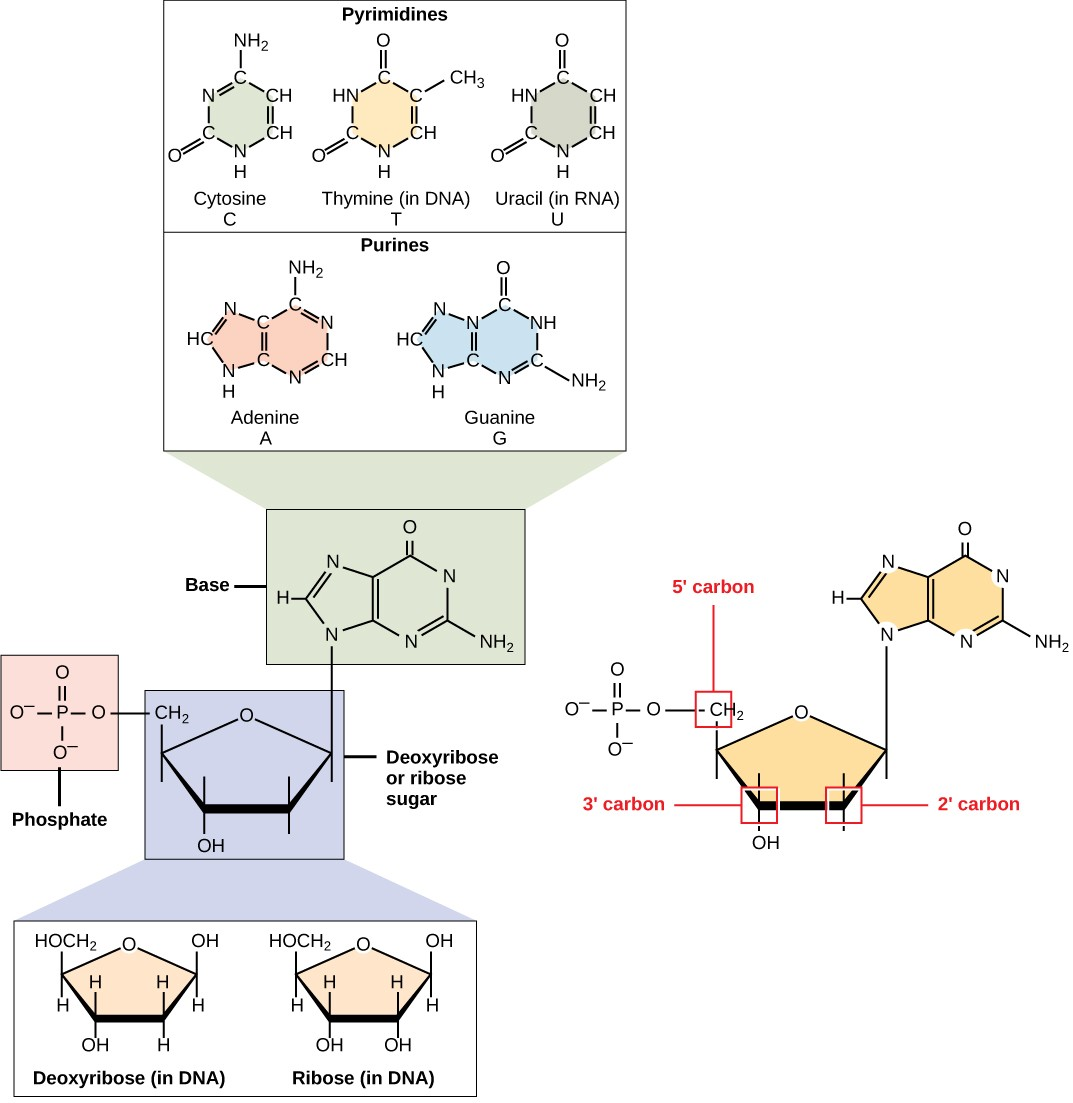
\includegraphics[width=14.9in]{/Users/nlb24/OneDrive - University of Pittsburgh/0-books/lbrb-bk/lbrb/./images/image5} \caption{A nucleotide is made up of three components: a nitrogenous base, a pentose sugar, and one or more phosphate groups. Carbon residues in the pentose are numbered 1′ through 5′ (the prime distinguishes these residues from those in the base, which are numbered without using a prime notation). The base is attached to the 1′ position of the ribose, and the phosphate is attached to the 5′ position. When a polynucleotide is formed, the 5′ phosphate of the incoming nucleotide attaches to the 3′ hydroxyl group at the end of the growing chain. Two types of pentose are found in nucleotides, deoxyribose (found in DNA) and ribose (found in RNA). Deoxyribose is similar in structure to ribose, but it has an H instead of an OH at the 2′ position. Bases can be divided into two categories: purines and pyrimidines. Purines have a double ring structure, and pyrimidines have a single ring.}\label{fig:unnamed-chunk-101}
\end{figure}

The nitrogenous bases, important components of nucleotides, are
organic molecules and are so named because they contain carbon and
nitrogen. They are bases because they contain an amino group that has
the potential of binding an extra hydrogen, and thus, decreases the
hydrogen ion concentration in its environment, making it more basic.
Each nucleotide in DNA contains one of four possible nitrogenous
bases: adenine (A), guanine (G) cytosine (C), and thymine (T).

Adenine and guanine are classified as purines. The primary structure
of a purine is two carbon-nitrogen rings. Cytosine, thymine, and
uracil are classified as pyrimidines which have a single
carbon-nitrogen ring as their primary structure (Figure 3.5.1). Each
of these basic carbon-nitrogen rings has different functional groups
attached to it. In molecular biology shorthand, the nitrogenous bases are simply known by their symbols A, T, G, C, and U. DNA contains A, T, G, and C whereas RNA contains A, U, G, and
C.

The pentose sugar in DNA is deoxyribose, and in RNA, the sugar is
ribose (Figure 3.5.1). The difference between the sugars is the
presence of the hydroxyl group on the second carbon of the ribose and
hydrogen on the second carbon of the deoxyribose. The carbon atoms of
the sugar molecule are numbered as 1′, 2′, 3′, 4′, and 5′ (1′ is read
as ``one prime''). The phosphate residue is attached to the hydroxyl
group of the 5′ carbon of one sugar and the hydroxyl group of the 3′
carbon of the sugar of the next nucleotide, which forms a 5′--3′
phosphodiester linkage. The phosphodiester linkage is not formed by
simple dehydration reaction like the other linkages connecting
monomers in macromolecules: its formation involves the removal of two
phosphate groups. A polynucleotide may have thousands of such
phosphodiester linkages.

\hypertarget{dna-double-helix-structure}{%
\section{DNA Double-Helix Structure}\label{dna-double-helix-structure}}

DNA has a double-helix structure (Figure 3.5.2). The sugar and
phosphate lie on the outside of the helix, forming the backbone of the
DNA. The nitrogenous bases are stacked in the interior, like the steps
of a staircase, in pairs; the pairs are bound to each other by
hydrogen bonds. Every base pair in the double helix is separated from
the next base pair by 0.34 nm. The two strands of the helix run in
opposite directions, meaning that the 5′ carbon end of one strand will
face the 3′ carbon end of its matching strand. (This is referred to as
antiparallel orientation and is important to DNA replication and in
many nucleic acid interactions.)

\begin{figure}
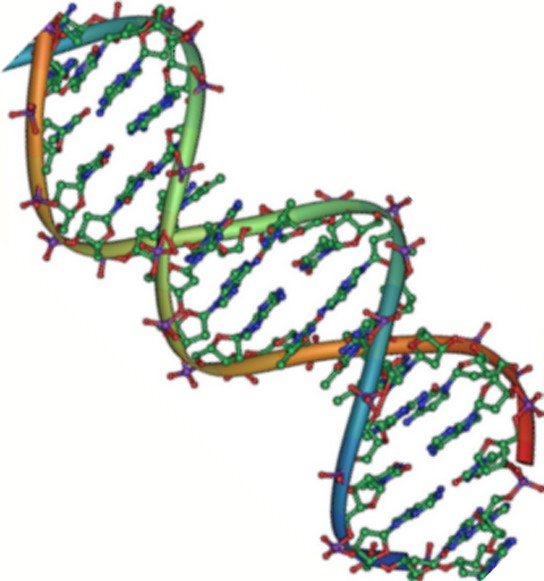
\includegraphics[width=7.56in]{/Users/nlb24/OneDrive - University of Pittsburgh/0-books/lbrb-bk/lbrb/./images/image6} \caption{Figure 3.5.2 : Native DNA is an antiparallel double helix. The phosphate backbone (indicated by the curvy lines) is on the outside, and the bases are on the inside. Each base from one strand interacts via hydrogen bonding with a base from the opposing strand. (credit: Jerome Walker/Dennis Myts)}\label{fig:unnamed-chunk-102}
\end{figure}

Only certain types of base pairing are allowed. For example, a certain
purine can only pair with a certain pyrimidine. This means A can pair
with T, and G can pair with C, as shown in Figure 3.5.3. This is known
as the base complementary rule. In other words, the DNA strands are
complementary to each other. If the sequence of one strand is
AATTGGCC, the complementary strand would have the sequence TTAACCGG.
During DNA replication, each strand is copied, resulting in a daughter
DNA double helix containing one parental DNA strand and a newly
synthesized strand.

Art Connection

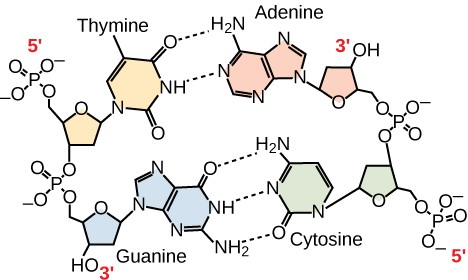
\includegraphics[width=6.5in]{/Users/nlb24/OneDrive - University of Pittsburgh/0-books/lbrb-bk/lbrb/./images/image7}

Figure 3.5.3 : In a double stranded DNA molecule, the two strands run
antiparallel to one another so that one strand runs 5′ to 3′ and the
other 3′ to 5′. The phosphate backbone is located on the outside, and
the bases are in the middle. Adenine forms hydrogen bonds (or base
pairs) with thymine, and guanine base pairs with cytosine.

A mutation occurs, and cytosine is replaced with adenine. What impact
do you think this will have on the DNA structure?

\hypertarget{rna}{%
\section{RNA}\label{rna}}

Ribonucleic acid, or RNA, is mainly involved in the process of protein
synthesis under the direction of DNA. RNA is usually single-stranded
and is made of ribonucleotides that are linked by phosphodiester
bonds. A ribonucleotide in the RNA chain contains ribose (the pentose
sugar), one of the four nitrogenous bases (A, U, G, and C), and the
phosphate group.

There are four major types of RNA: messenger RNA (mRNA), ribosomal RNA
(rRNA), transfer RNA (tRNA), and microRNA (miRNA). The first, mRNA,
carries the message from DNA, which controls all of the cellular
activities in a cell. If a cell requires a certain protein to be
synthesized, the gene for this product is turned ``on'' and the
messenger RNA is synthesized in the nucleus. The RNA base sequence is
complementary to the coding sequence of the DNA from which it has been
copied. However, in RNA, the base T is absent and U is present
instead. If the DNA strand has a sequence AATTGCGC, the sequence of
the complementary RNA is UUAACGCG. In the cytoplasm, the mRNA
interacts with ribosomes and other cellular machinery (Figure 3.5.4).

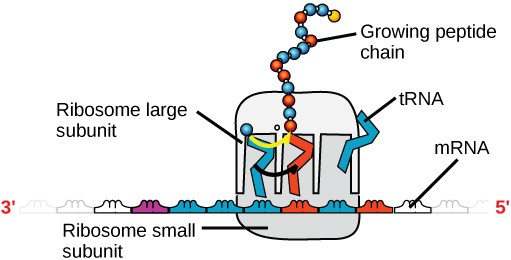
\includegraphics[width=7.1in]{/Users/nlb24/OneDrive - University of Pittsburgh/0-books/lbrb-bk/lbrb/./images/image8}

Figure 3.5.4 : A ribosome has two parts: a large subunit and a small
subunit. The mRNA sits in between the two subunits. A tRNA molecule
recognizes a codon on the mRNA, binds to it by complementary base
pairing, and adds the correct amino acid to the growing peptide chain.

The mRNA is read in sets of three bases known as codons. Each codon
codes for a single amino acid. In this way, the mRNA is read and the
protein product is made. Ribosomal RNA (rRNA) is a major constituent
of ribosomes on which the mRNA binds. The rRNA ensures the proper
alignment of the mRNA and the ribosomes; the rRNA of the ribosome also
has an enzymatic activity (peptidyl transferase) and catalyzes the
formation of the peptide bonds between two aligned amino acids.
Transfer RNA (tRNA) is one of the smallest of the four types of RNA,
usually 70--90 nucleotides long. It carries the correct amino acid to
the site of protein synthesis. It is the base pairing between the tRNA
and mRNA that allows for the correct amino acid to be inserted in the
polypeptide chain. microRNAs are the smallest RNA molecules and their
role involves the regulation of gene expression by interfering with
the expression of certain mRNA messages. Table 3.5.1 below summarizes
features of DNA and RNA.

\textbf{\emph{Table}} 3.5.1 *\textbf{:} Features of DNA and RNA.

\begin{longtable}[]{@{}
  >{\raggedright\arraybackslash}p{(\columnwidth - 4\tabcolsep) * \real{0.31}}
  >{\raggedright\arraybackslash}p{(\columnwidth - 4\tabcolsep) * \real{0.35}}
  >{\raggedright\arraybackslash}p{(\columnwidth - 4\tabcolsep) * \real{0.35}}@{}}
\toprule
\begin{minipage}[b]{\linewidth}\raggedright
\end{minipage} & \begin{minipage}[b]{\linewidth}\raggedright
Features of DNA and
RNA
\end{minipage} & \begin{minipage}[b]{\linewidth}\raggedright
\end{minipage} \\
\midrule
\endhead
& DNA & RNA \\
Function & Carries genetic
information & Involved in protein
synthesis \\
Location & Remains in the nucleus & Leaves the nucleus \\
Structure & Double helix & Usually
single-stranded \\
Sugar & Deoxyribose & Ribose \\
Pyrimidines & Cytosine, thymine & Cytosine, uracil \\
Purines & Adenine, guanine & Adenine, guanine \\
\bottomrule
\end{longtable}

Even though the RNA is single stranded, most RNA types show extensive
intramolecular base pairing between complementary sequences, creating
a predictable three-dimensional structure essential for their
function.

As you have learned, information flow in an organism takes place from
DNA to RNA to protein. DNA dictates the structure of mRNA in a process
known as transcription, and RNA dictates the structure of protein in a
process known as translation. This is known as the Central Dogma of
Life, which holds true for all organisms; however, exceptions to the
rule occur in connection with viral infections.

\emph{Link to Learning}


\includegraphics[width=0.1\linewidth]{/Users/nlb24/OneDrive - University of Pittsburgh/0-books/lbrb-bk/lbrb/./images/image9}

\begin{itemize}
\tightlist
\item
  To learn more about DNA, explore the Howard Hughes Medical Institute
  BioInteractive animations on the topic of DNA.*
\end{itemize}

\hypertarget{summary}{%
\section{Summary}\label{summary}}

Nucleic acids are molecules made up of nucleotides that direct
cellular activities such as cell division and protein synthesis. Each
nucleotide is made up of a pentose sugar, a nitrogenous base, and a
phosphate group. There are two types of nucleic acids: DNA and RNA.
DNA carries the genetic blueprint of the cell and is passed on from
parents to offspring (in the form of chromosomes). It has a
double-helical structure with the two strands running in opposite
directions, connected by hydrogen bonds, and complementary to each
other. RNA is single-stranded and is made of a pentose sugar (ribose),
a nitrogenous base, and a phosphate group. RNA is involved in protein
synthesis and its regulation. Messenger RNA (mRNA) is copied from the
DNA, is exported from the nucleus to the cytoplasm, and contains
information for the construction of proteins. Ribosomal RNA (rRNA) is
a part of the ribosomes at the site of protein synthesis, whereas
transfer RNA (tRNA) carries the amino acid to the site of protein
synthesis. microRNA regulates the use of mRNA for protein synthesis.

Art Connections

\hypertarget{analysis-questions}{%
\section{Analysis Questions}\label{analysis-questions}}

Free Response

\hypertarget{glossary}{%
\section{Glossary}\label{glossary}}

\textbf{deoxyribonucleic acid (DNA)}: double-helical molecule that carries the hereditary information of the cell\\
\textbf{messenger RNA (mRNA)}: DNA that carries information from DNA to ribosomes during protein synthesis\\
\textbf{nucleic acid}: biological macromolecule that carries the genetic blueprint of a cell
and carries instructions for the functioning of the cell\\
\textbf{nucleotide}: monomer of nucleic acids; contains a pentose sugar, one or more phosphate groups, and a nitrogenous base\\
\textbf{phosphodiester}: linkage covalent chemical bond that holds together the polynucleotide
chains with a phosphate group linking two pentose sugars of neighboring nucleotides\\
\textbf{polynucleotide}: long chain of nucleotides\\
\textbf{purine}: type of nitrogenous base in DNA and RNA; adenine and guanine are\\
\textbf{purines, pyrimidine}: type of nitrogenous base in DNA and RNA; cytosine, thymine, and uracil
are pyrimidines\\
\textbf{ribonucleic acid (RNA)}: single-stranded, often internally base paired, molecule that is
involved in protein synthesis\\
\textbf{ribosomal RNA (rRNA)}: RNA that ensures the proper alignment of the mRNA and the ribosomes
during protein synthesis and catalyzes the formation of the peptide linkage\\
\textbf{transcription}: process through which messenger RNA forms on a template of DNA\\
\textbf{transfer RNA (tRNA)}: RNA that carries activated amino acids to the site of protein
synthesis on the ribosome\\
\textbf{translation}: process through which RNA directs the formation of protein

\hypertarget{contributors-and-attributions}{%
\section{Contributors and Attributions}\label{contributors-and-attributions}}

Connie Rye (East Mississippi Community College), Robert Wise
(University of Wisconsin, Oshkosh), Vladimir Jurukovski (Suffolk
County Community College), Jean DeSaix (University of North Carolina
at Chapel Hill), Jung Choi (Georgia Institute of Technology), Yael
Avissar (Rhode Island College) among other contributing authors.
Original content by OpenStax (CC BY 4.0; Download for free at
\href{http://cnx.org/contents/185cbf87-c72e-48f5-b51e-f14f21b5eabd\%409.87}{http://cnx.org/contents/185cbf87-c72...f21b5eabd@9.87}).

\hypertarget{proteins-review}{%
\chapter{Proteins}\label{proteins-review}}

\textbf{Authors}: OpenStax / LibreText. Formatted in RMarkdown by Nathan Brouwer under the Creative Commons Attribution License 4.0 license.

This chapter was adapted from \href{}{LibreText General Biology}, Chapter 3, Section 3.4: \href{https://bio.libretexts.org/Bookshelves/Introductory_and_General_Biology/Book\%3A_General_Biology_(OpenStax)/1\%3A_The_Chemistry_of_Life/3\%3A_Biological_Macromolecules/3.4\%3A_Proteins}{Proteins}. The LibreText book is based on \href{https://openstax.org/details/books/biology-2e}{OpenStax Biology 2nd edition}, Chapter 3, Section 3.4: \href{https://openstax.org/books/biology-2e/pages/3-4-proteins}{Nucleic Acids}. A full list of authors is found under the \textbf{Contributors and Attributions} section at the end of this document.

\hypertarget{skills-to-develop}{%
\subsection{Skills to develop:}\label{skills-to-develop}}

\begin{enumerate}
\def\labelenumi{\arabic{enumi}.}
\tightlist
\item
  Describe the functions proteins perform in the cell and in tissues
\item
  Discuss the relationship between amino acids and proteins
\item
  Explain the four levels of protein organization
\item
  Describe the ways in which protein shape and function are linked
\end{enumerate}

Proteins are one of the most abundant organic molecules in living systems and have the most diverse range of functions of all \textbf{macromolecules}. Proteins may be structural, regulatory, contractile, or protective; they may serve in transport, storage, or membranes; or they may be toxins or enzymes. Each cell in a living system may contain thousands of proteins, each with a unique function. Their structures, like their functions, vary greatly. They are all, however, \textbf{polymers} of \textbf{amino acids}, arranged in a linear sequence.

\hypertarget{types-and-functions-of-proteins}{%
\section{Types and Functions of Proteins}\label{types-and-functions-of-proteins}}

\textbf{Enzymes}, which are produced by living cells, are \textbf{catalysts} in biochemical reactions (like digestion) and are usually complex or conjugated proteins. Each enzyme is specific for the substrate (a reactant that binds to an enzyme) it acts on. The enzyme may help in breakdown, rearrangement, or synthesis reactions. Enzymes that break down their substrates are called \textbf{catabolic enzymes}, enzymes that build more complex molecules from their substrates are called \textbf{anabolic enzymes}, and enzymes that affect the rate of reaction are called \textbf{catalytic enzymes}.
It should be noted that all enzymes increase the rate of reaction and, therefore, are considered to be organic catalysts. An example of an enzyme is salivary amylase, which
hydrolyzes its substrate amylose, a component of starch.

\textbf{Hormones} are chemical-signaling molecules, usually small proteins or steroids, secreted by endocrine cells that act to control or regulate specific physiological processes, including growth, development, metabolism, and reproduction. For example, insulin is a \textbf{protein hormone} that helps to regulate the blood glucose level.

Proteins have different shapes and molecular weights; some proteins are \textbf{globular} in shape whereas others are fibrous. For example, hemoglobin is a globular protein, but collagen, found in our skin, is a fibrous protein. Protein shape is critical to its function, and this shape is maintained by many different types of chemical bonds. Changes in temperature, pH, and exposure to chemicals may lead to permanent changes in the shape of the protein, leading to loss of function, known as \textbf{denaturation}. All proteins are made up of different arrangements of the same 20 types of \textbf{amino acids}.

\hypertarget{amino-acids}{%
\section{Amino Acids}\label{amino-acids}}

Amino acids are the \textbf{monomers} that make up proteins. Each amino acid has the same fundamental structure, which consists of a central carbon atom, also known as the alpha (\emph{α}) carbon, bonded to an amino group (NH\textsubscript{2}), a carboxyl group (COOH), and to a hydrogen atom. Every amino acid also has another atom or group of atoms bonded to the central atom known as the R group (Figure 3.4.1).

\begin{figure}
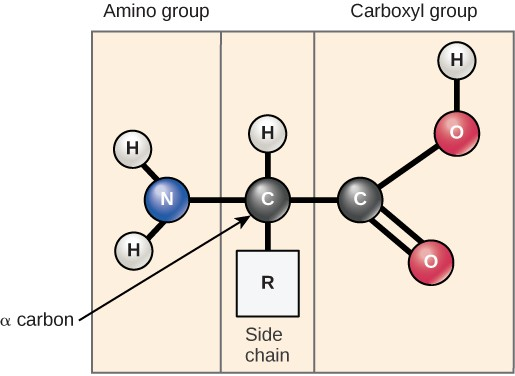
\includegraphics[width=7.15in]{/Users/nlb24/OneDrive - University of Pittsburgh/0-books/lbrb-bk/lbrb/./images/protimage1} \caption{Amino acids have a central asymmetric carbon to which an amino group, a carboxyl group, a hydrogen atom, and a side chain (R group) are attached.}\label{fig:unnamed-chunk-106}
\end{figure}

The name ``amino acid'' is derived from the fact that they contain both an amino group and carboxyl-acid-group in their basic structure. For each amino acid, the R group (or side chain) is different (Figure 3.4.2).

\begin{figure}
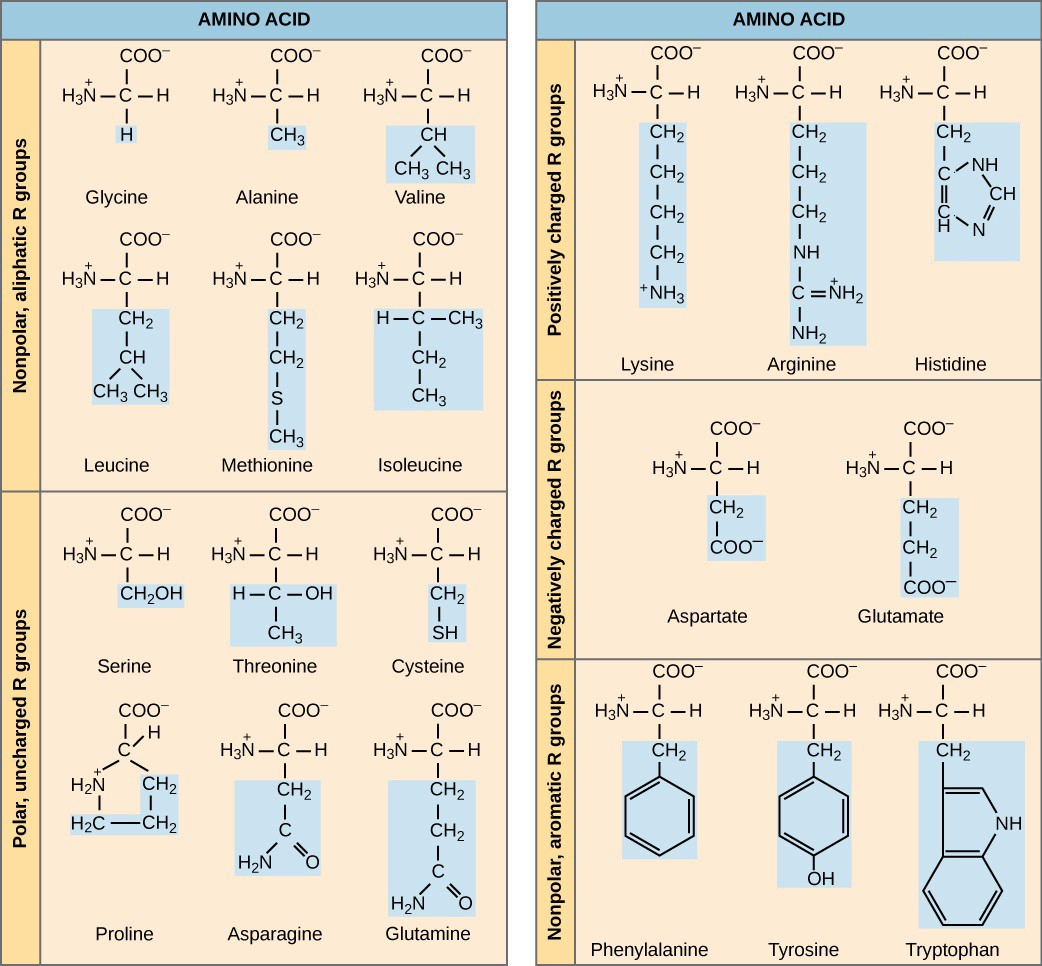
\includegraphics[width=0.6\linewidth]{/Users/nlb24/OneDrive - University of Pittsburgh/0-books/lbrb-bk/lbrb/./images/protimage2} \caption{There are 20 common amino acids commonly found in proteins, each with a different R group (variant group) that determines its chemical nature.}\label{fig:unnamed-chunk-107}
\end{figure}

Which categories of amino acid would you expect to find on the surface
of a soluble protein, and which would you expect to find in the
interior? What distribution of amino acids would you expect to find in
a protein embedded in a lipid bilayer?

The chemical nature of the side chain determines the nature of the amino acid (that is, whether it is \textbf{acidic}, \textbf{basic}, \textbf{polar}, or \textbf{nonpolar}). For example, the amino acid glycine has a hydrogen atom as the R group. Amino acids such as valine, methionine, and alanine are nonpolar or hydrophobic, while amino acids such as serine, threonine, and cysteine are polar and have hydrophilic side chains. The side chains of lysine and arginine are positively charged, and therefore these amino acids are also known as basic amino acids. Proline has an R group that is linked to the amino group, forming a ring-like structure. Proline is an exception to the standard structure of an amino acid since its amino group is not separate from the side chain

Amino acids are represented by a single upper case letter or a three-letter abbreviation. For example, valine is known by the letter V or the three-letter code val.

The sequence and the number of amino acids ultimately determine a protein's shape, size, and function. Each amino acid is attached to another amino acid by a covalent bond, known as a \textbf{peptide bond}, which is formed by a dehydration reaction. The carboxyl group of one amino acid and the amino group of the incoming amino acid combine, releasing a molecule of water. The resulting bond is the peptide bond

\begin{figure}
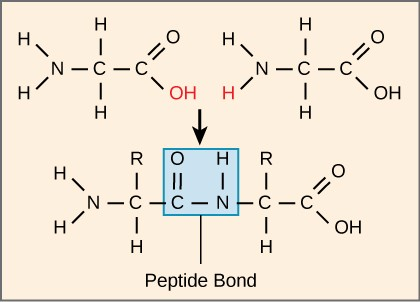
\includegraphics[width=5.83in]{/Users/nlb24/OneDrive - University of Pittsburgh/0-books/lbrb-bk/lbrb/./images/protimage3} \caption{Peptide bond formation is a dehydration synthesis reaction. The carboxyl group of one amino acid is linked to the amino group of the incoming amino acid. In the process, a molecule of water is released.}\label{fig:unnamed-chunk-108}
\end{figure}

The products formed by such linkages are called \textbf{peptides}. As more amino acids join to this growing chain, the resulting chain is known as a \textbf{polypeptide}. Each polypeptide has a free amino group at one end. This end is called the \textbf{N-terminal}, or the amino terminal, and the other end has a free carboxyl group, also known as the C- or carboxyl
terminal. The terms polypeptide and protein are sometimes used interchangeably, a polypeptide is technically a polymer of amino acids, whereas the term protein is more formally used for a polypeptide or that have combined together, often have bound non-peptide prosthetic groups, have a distinct shape, and have a unique function.

After \textbf{protein synthesis (translation)}, most proteins are modified. These are known as \textbf{post-translational modifications}. They may undergo \textbf{cleavage}, \textbf{phosphorylation} (addition of a phosphate group), or may require the addition of other chemical groups. Only after these modifications is the protein completely functional.

\hypertarget{evolution-connection}{%
\section{Evolution Connection:}\label{evolution-connection}}

\begin{center}\rule{0.5\linewidth}{0.5pt}\end{center}

\textbf{The Evolutionary Significance of Cytochrome}: Cytochrome c is an
important component of the electron transport chain, a part of
cellular respiration, and it is normally found in the cellular
organelle, the mitochondrion. This protein has a heme prosthetic
group, and the central ion of the heme gets alternately reduced and
oxidized during electron transfer. Because this essential protein's
role in producing cellular energy is crucial, it has changed very
little over millions of years. Protein sequencing has shown that there
is a considerable amount of cytochrome c amino acid sequence \textbf{homology}
among different species; in other words, evolutionary kinship can be
assessed by measuring the similarities or differences among various
species' DNA or protein sequences.

Scientists have determined that human cytochrome c contains 104 amino
acids. For each cytochrome c molecule from different organisms that
has been sequenced to date, 37 of these amino acids appear in the same
position in all samples of cytochrome c.~This indicates that there may
have been a \textbf{common ancestor}. On comparing the human and chimpanzee
protein sequences, no sequence difference was found. When human and
rhesus monkey sequences were compared, the single difference found was
in one amino acid. In another comparison, human to yeast sequencing
shows a difference in the 44th position.

\begin{center}\rule{0.5\linewidth}{0.5pt}\end{center}

\hypertarget{protein-structure}{%
\section{Protein Structure}\label{protein-structure}}

The shape of a protein is critical to its function. For example, an enzyme can bind to a specific substrate at a site known as the \textbf{active site}. If this active site is altered because of local changes or changes in overall protein structure, the enzyme may be unable to bind to the substrate. To understand how the protein gets its final shape or conformation, we need to understand the four levels of protein structure: primary, secondary, tertiary, and quaternary.

\hypertarget{primary-structure}{%
\subsection{Primary Structure}\label{primary-structure}}

The unique sequence of amino acids in a polypeptide chain is its
primary structure. For example, the pancreatic hormone insulin has two
polypeptide chains, A and B, and they are linked together by disulfide
bonds. The N terminal amino acid of the A chain is glycine, whereas
the C terminal amino acid is asparagine (Figure 3.4.4). The sequences
of amino acids in the A and B chains are unique to insulin.

\begin{figure}
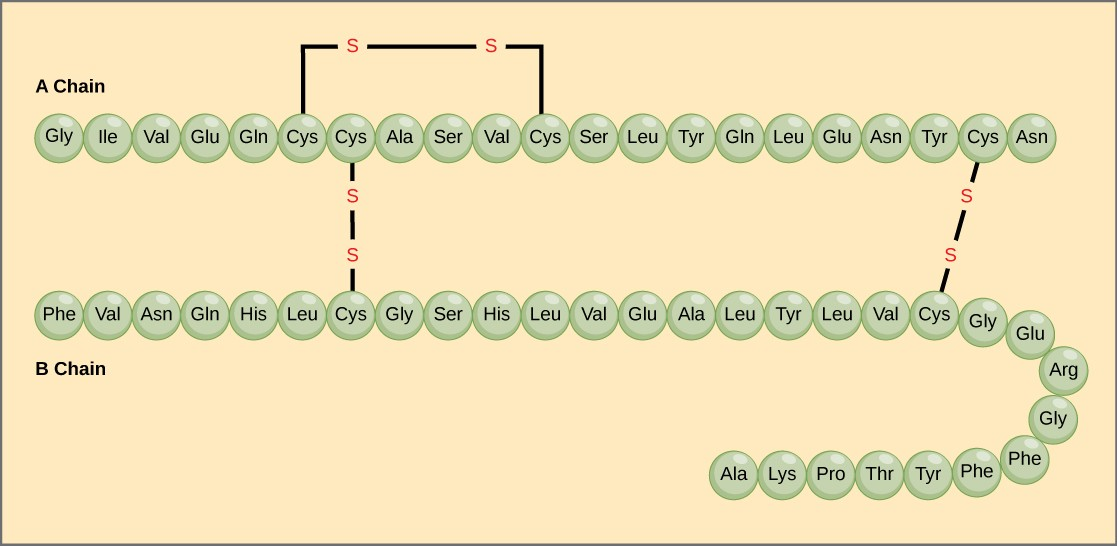
\includegraphics[width=0.4\linewidth]{/Users/nlb24/OneDrive - University of Pittsburgh/0-books/lbrb-bk/lbrb/./images/protimage4} \caption{Bovine serum insulin is a protein hormone made of two peptide chains, A (21 amino acids long) and B (30 amino acids long). In each chain, primary structure is indicated by three-letter abbreviations that represent the names of the amino acids in the order they are present. The amino acid cysteine (cys) has a sulfhydryl (SH) group as a side chain. Two sulfhydryl groups can react in the presence of oxygen to form a disulfide (S-S) bond. Two disulfide bonds connect the A and B chains together, and a third helps the A chain fold into the correct shape. Note that all disulfide bonds are the same length, but are drawn different sizes for clarity.}\label{fig:unnamed-chunk-109}
\end{figure}

The unique sequence for every protein is ultimately determined by the
gene encoding the protein. A change in nucleotide sequence of the
gene's coding region may lead to a different amino acid being added to
the growing polypeptide chain, causing a change in protein structure
and function. In sickle cell anemia, the hemoglobin \emph{beta} chain (a small
portion of which is shown in Figure 3.4.5) has a single amino acid
substitution, causing a change in protein structure and function.
Specifically, the amino acid glutamic acid is substituted by valine in
the beta chain. What is most remarkable to consider is that a
hemoglobin molecule is made up of two alpha chains and two beta chains
that each consist of about 150 amino acids. The molecule, therefore,
has about 600 amino acids. The structural difference between a normal
hemoglobin molecule and a sickle cell molecule---which dramatically
decreases life expectancy---is a single amino acid of the 600. What is
even more remarkable is that those 600 amino acids are encoded by
three nucleotides each, and the mutation is caused by a single base
change (point mutation), 1 in 1800 bases.

\begin{figure}
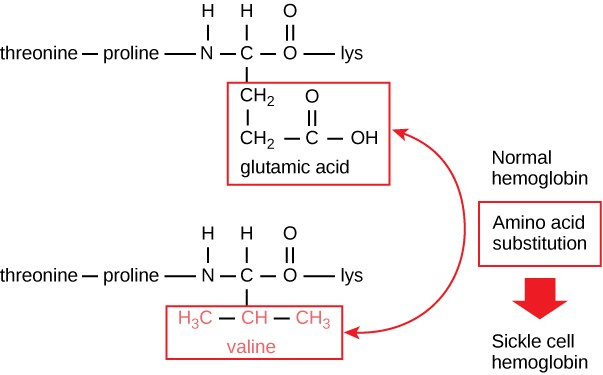
\includegraphics[width=0.4\linewidth]{/Users/nlb24/OneDrive - University of Pittsburgh/0-books/lbrb-bk/lbrb/./images/protimage5} \caption{The beta chain of hemoglobin is 147 residues in length, yet a single amino acid substitution leads to sickle cell anemia. In normal hemoglobin, the amino acid at position seven is glutamate. In sickle cell hemoglobin, this glutamate is replaced by a valine.}\label{fig:unnamed-chunk-110}
\end{figure}

Because of this change of one amino acid in the chain, hemoglobin
molecules form long fibers that distort the biconcave, or disc-shaped,
red blood cells and assume a crescent or ``sickle'' shape, which clogs
arteries (Figure 3.4.6). This can lead to myriad serious health
problems such as breathlessness, dizziness, headaches, and abdominal
pain for those affected by this disease.

\begin{figure}
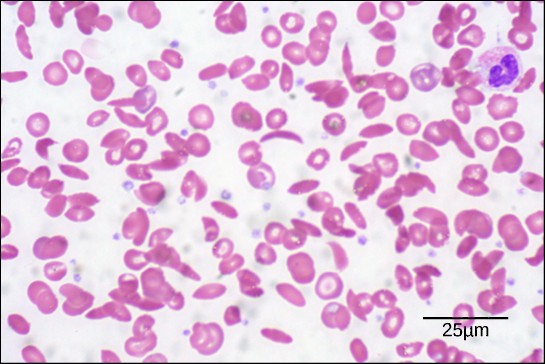
\includegraphics[width=0.6\linewidth]{/Users/nlb24/OneDrive - University of Pittsburgh/0-books/lbrb-bk/lbrb/./images/protimage6} \caption{In this blood smear, visualized at 535x magnification using bright field microscopy, sickle cells are crescent shaped, while normal cells are disc-shaped. (credit: modification of work by Ed Uthman; scale-bar data from Matt Russell)}\label{fig:unnamed-chunk-111}
\end{figure}

\hypertarget{secondary-structure}{%
\subsection{Secondary Structure}\label{secondary-structure}}

The local folding of the polypeptide in some regions gives rise to the
secondary structure of the protein. The most common are the \emph{α}-helix
and \emph{beta}-pleated sheet structures (Figure 3.4.7). Both structures are
the \emph{α}-helix structure---the helix held in shape by hydrogen bonds.
The hydrogen bonds form between the oxygen atom in the carbonyl group
in one amino acid and another amino acid that is four amino acids
farther along the chain.

\begin{figure}
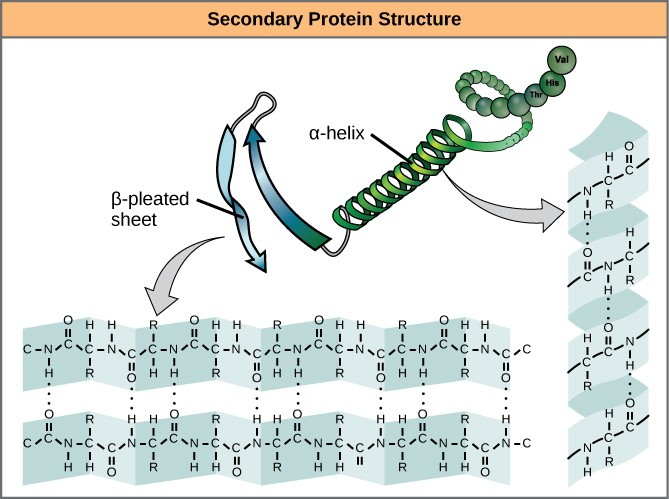
\includegraphics[width=0.4\linewidth]{/Users/nlb24/OneDrive - University of Pittsburgh/0-books/lbrb-bk/lbrb/./images/protimage7} \caption{The α-helix and β-pleated sheet are secondary structures of proteins that form because of hydrogen bonding between carbonyl and amino groups in the peptide backbone. Certain amino acids have a propensity to form an α-helix, while others have a propensity to form a β-pleated sheet.}\label{fig:unnamed-chunk-112}
\end{figure}

Every helical turn in an alpha helix has 3.6 amino acid residues. The
R groups (the variant groups) of the polypeptide protrude out from the
\emph{α}-helix chain. In the \emph{beta}-pleated sheet, the ``pleats'' are formed by
hydrogen bonding between atoms on the backbone of the polypeptide
chain. The R groups are attached to the carbons and extend above and
below the folds of the pleat. The pleated segments align parallel or
antiparallel to each other, and hydrogen bonds form between the
partially positive nitrogen atom in the amino group and the partially
negative oxygen atom in the carbonyl group of the peptide backbone.
The \emph{α}-helix and \emph{beta}-pleated sheet structures are found in most
globular and fibrous proteins and they play an important structural
role.

\hypertarget{tertiary-structure}{%
\subsection{Tertiary Structure}\label{tertiary-structure}}

The unique three-dimensional structure of a polypeptide is its
tertiary structure (Figure 3.4.8). This structure is in part due to
chemical interactions at work on the polypeptide chain. Primarily, the
interactions among R groups creates the complex three- dimensional
tertiary structure of a protein. The nature of the R groups found in
the amino acids involved can counteract the formation of the hydrogen
bonds described for standard secondary structures. For example, R
groups with like charges are repelled by each other and those with
unlike charges are attracted to each other (ionic bonds). When protein
folding takes place, the hydrophobic R groups of nonpolar amino acids
lay in the interior of the protein, whereas the hydrophilic R groups
lay on the outside. The former types of interactions are also known as
hydrophobic interactions. Interaction between cysteine side chains
forms disulfide linkages in the presence of oxygen, the only covalent
bond forming during protein folding.

\begin{figure}
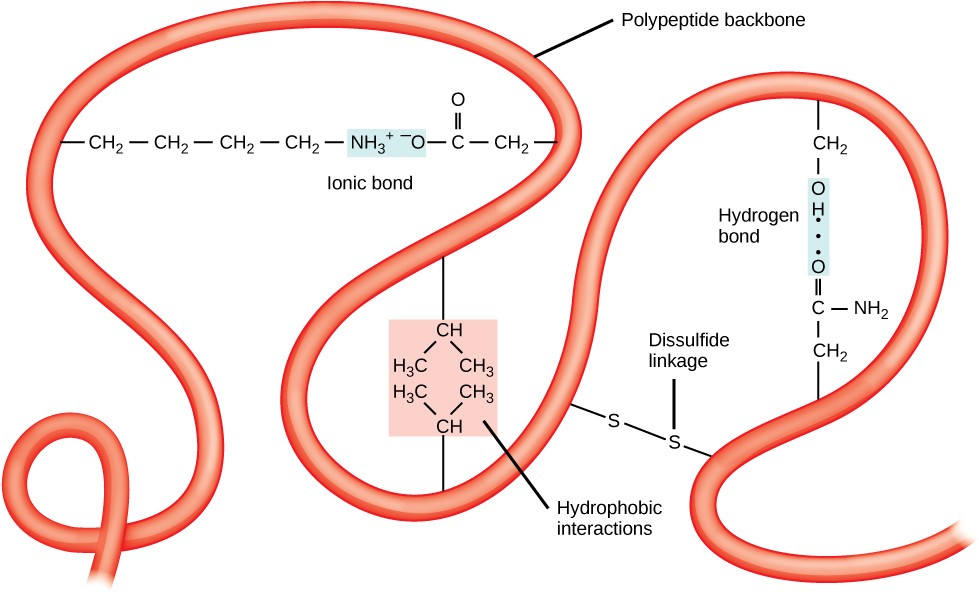
\includegraphics[width=0.4\linewidth]{/Users/nlb24/OneDrive - University of Pittsburgh/0-books/lbrb-bk/lbrb/./images/protimage8} \caption{The tertiary structure of proteins is determined by a variety of chemical interactions. These include hydrophobic interactions, ionic bonding, hydrogen bonding and disulfide linkages.}\label{fig:unnamed-chunk-113}
\end{figure}

All of these interactions, weak and strong, determine the final
three-dimensional shape of the protein. When a protein loses its
three-dimensional shape, it may no longer be functional.

\hypertarget{quaternary-structure}{%
\subsection{Quaternary Structure}\label{quaternary-structure}}

In nature, some proteins are formed from several polypeptides, also
known as subunits, and the interaction of these subunits forms the
quaternary structure. Weak interactions between the subunits help to
stabilize the overall structure. For example, insulin (a globular
protein) has a combination of hydrogen bonds and disulfide bonds that
cause it to be mostly clumped into a ball shape. Insulin starts out as
a single polypeptide and loses some internal sequences in the presence
of post-translational modification after the formation of the
disulfide linkages that hold the remaining chains together. Silk (a
fibrous protein), however, has a \emph{beta}-pleated sheet structure that is
the result of hydrogen bonding between different chains.

The four levels of protein structure (primary, secondary, tertiary,
and quaternary) are illustrated in Figure 3.4.9.

\begin{figure}
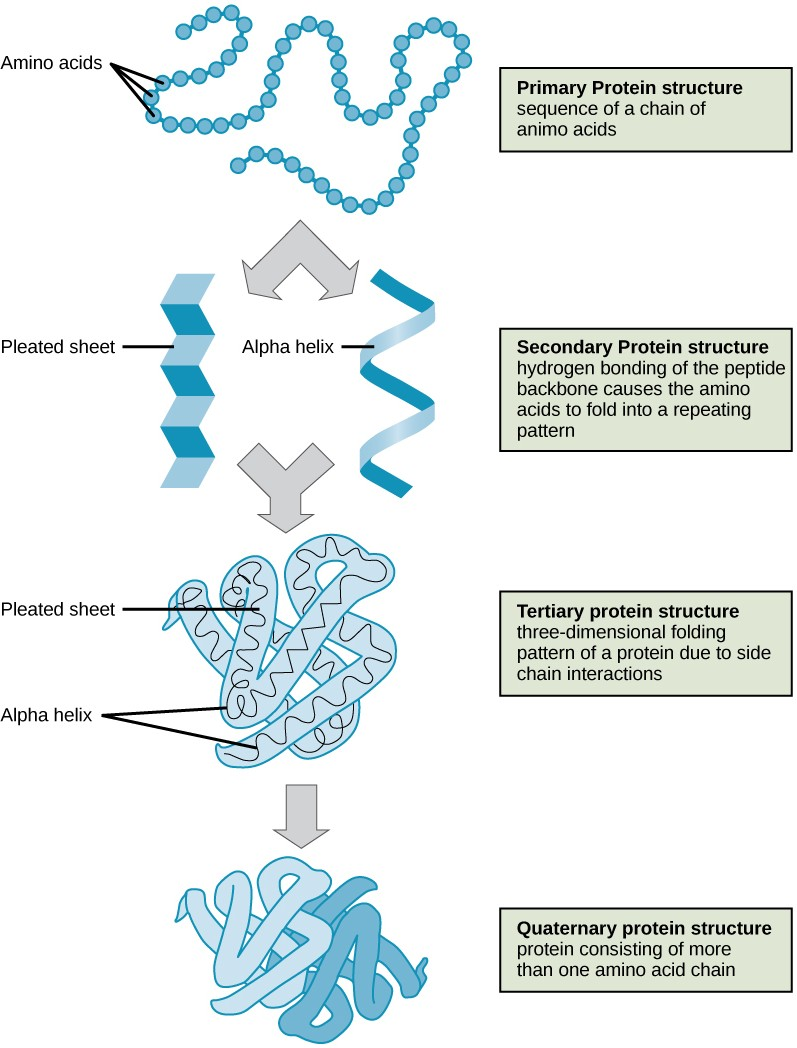
\includegraphics[width=11.07in]{/Users/nlb24/OneDrive - University of Pittsburgh/0-books/lbrb-bk/lbrb/./images/protimage9} \caption{The four levels of protein structure can be observed in these illustrations. (credit: modification of work by National Human Genome Research Institute)}\label{fig:unnamed-chunk-114}
\end{figure}

\hypertarget{denaturation-and-protein-folding}{%
\section{Denaturation and Protein Folding}\label{denaturation-and-protein-folding}}

Each protein has its own unique sequence and shape that are held
together by chemical interactions. If the protein is subject to
changes in temperature, pH, or exposure to chemicals, the protein
structure may change, losing its shape without losing its primary
sequence in what is known as denaturation. Denaturation is often
reversible because the primary structure of the polypeptide is
conserved in the process if the denaturing agent is removed, allowing
the protein to resume its function. Sometimes denaturation is
irreversible, leading to loss of function. One example of irreversible
protein denaturation is when an egg is fried. The albumin protein in
the liquid egg white is denatured when placed in a hot pan. Not all
proteins are denatured at high temperatures; for instance, bacteria
that survive in hot springs have proteins that function at
temperatures close to boiling. The stomach is also very acidic, has a
low pH, and denatures proteins as part of the digestion process;
however, the digestive enzymes of the stomach retain their activity
under these conditions.

Protein folding is critical to its function. It was originally thought
that the proteins themselves were responsible for the folding process.
Only recently was it found that often they receive assistance in the
folding process from protein helpers known as chaperones (or
chaperonins) that associate with the target protein during the folding
process. They act by preventing aggregation of polypeptides that make
up the complete protein structure, and they disassociate from the
protein once the target protein is folded.

\hypertarget{summary-1}{%
\section{Summary}\label{summary-1}}

Proteins are a class of macromolecules that perform a diverse range of
functions for the cell. They help in metabolism by providing
structural support and by acting as enzymes, carriers, or hormones.
The building blocks of proteins (monomers) are amino acids. Each amino
acid has a central carbon that is linked to an amino group, a carboxyl
group, a hydrogen atom, and an

R group or side chain. There are 20 commonly occurring amino acids,
each of which differs in the R group. Each amino acid is linked to its
neighbors by a peptide bond. A long chain of amino acids is known as a
polypeptide.

Proteins are organized at four levels: primary, secondary, tertiary,
and (optional) quaternary. The primary structure is the unique
sequence of amino acids. The local folding of the polypeptide to form
structures such as the \emph{α} helix and \emph{beta}-pleated sheet constitutes the
secondary structure. The overall three-dimensional structure is the
tertiary structure. When two or more polypeptides combine to form the
complete protein structure, the configuration is known as the
quaternary structure of a protein. Protein shape and function are
intricately linked; any change in shape caused by changes in
temperature or pH may lead to protein denaturation and a loss in
function.

\hypertarget{art-connections}{%
\section{Art Connections}\label{art-connections}}

\begin{itemize}
\item
  Which categories of amino acid would you expect to find on
  the surface of a soluble protein, and which would you expect to find
  in the interior? What distribution of amino acids would you expect to
  find in a protein embedded in a lipid bilayer?
\item
  Polar and charged amino acid residues (the remainder after
  peptide bond formation) are more likely to be found on the surface of
  soluble proteins where they can interact with water, and nonpolar
  (e.g., amino acid side chains) are more likely to be found in the
  interior where they are sequestered from water. In membrane proteins,
  nonpolar and hydrophobic amino acid side chains associate with the
  hydrophobic tails of phospholipids, while polar and charged amino acid
  side chains interact with the polar head groups or with the aqueous
  solution. However, there are exceptions. Sometimes, positively and
  negatively charged amino acid side chains interact with one another in
  the interior of a protein, and polar or charged amino acid side chains
  that interact with a ligand can be found in the ligand binding pocket.
\end{itemize}

\hypertarget{review-questions}{%
\section{Review Questions}\label{review-questions}}

The monomers that make up proteins are called
1. nucleotides
1. disaccharides
1. amino acids
1. chaperones

Answer: C

The \emph{α} helix and the \emph{beta}-pleated sheet are part of which protein
structure?

\begin{enumerate}
\def\labelenumi{\arabic{enumi}.}
\tightlist
\item
  primary
\item
  secondary
\item
  tertiary
\item
  quaternary
\end{enumerate}

Answer: B

\hypertarget{free-response}{%
\section{Free Response}\label{free-response}}

\textbf{Explain what happens if even one amino acid is substituted for another
in a polypeptide chain. Provide a specific example.}

A change in gene sequence can lead to a different amino acid being
added to a polypeptide chain instead of the normal one. This causes a
change in protein structure and function. For example, in sickle cell
anemia, the hemoglobin \emph{beta} chain has a single amino acid
substitution---the amino acid glutamic acid in position six is
substituted by valine. Because of this change, hemoglobin molecules
form aggregates, and the disc-shaped red blood cells assume a crescent
shape, which results in serious health problems.

\textbf{Describe the differences in the four protein structures.}

The sequence and number of amino acids in a polypeptide chain is its
primary structure. The local folding of the polypeptide in some
regions is the secondary structure of the protein. The
three-dimensional structure of a polypeptide is known as its tertiary
structure, created in part by chemical interactions such as hydrogen
bonds between polar side chains, van der Waals interactions, disulfide
linkages, and hydrophobic interactions. Some proteins are formed from
multiple polypeptides, also known as subunits, and the interaction of
these subunits forms the quaternary structure.

\hypertarget{glossary-1}{%
\section{Glossary}\label{glossary-1}}

\textbf{alpha-helix structure (\emph{α}-helix)}: type of secondary structure of proteins formed by folding of the polypeptide into a helix shape with hydrogen bonds stabilizing the
structure\\
\textbf{amino acid}: monomer of a protein; has a central carbon or alpha carbon to which an
amino group, a carboxyl group, a hydrogen, and an R group or side
chain is attached; the R group is different for all 20 amino acids\\
\textbf{beta-pleated sheet (\emph{beta}-pleated)}: secondary structure found in proteins in which ``pleats'' are formed by hydrogen bonding between atoms on the backbone of the polypeptide chain\\
\textbf{chaperone}: (also, chaperonin) protein that helps nascent protein in the folding process \textbf{denaturation}: loss of shape in a protein as a result of changes in temperature, pH, or exposure to chemicals\\
\textbf{enzyme}: catalyst in a biochemical reaction that is usually a complex or conjugated protein\\
\textbf{hormone}: chemical signaling molecule, usually protein or steroid, secreted by endocrine cells that act to control or regulate specific physiological processes
\textbf{peptide bond}: bond formed between two amino acids by a dehydration reaction\\
\textbf{polypeptide}: long chain of amino acids linked by peptide bonds\\
\textbf{primary structure}: linear sequence of amino acids in a protein\\
\textbf{protein}: biological macromolecule composed of one or more chains of amino acids\\
\textbf{quaternary structure}: association of discrete polypeptide subunits in a protein\\
\textbf{secondary structure}: regular structure formed by proteins by intramolecular hydrogen bonding between the oxygen atom of one amino acid residue and the hydrogen attached to the nitrogen atom of another amino acid residue
\textbf{tertiary structure}: three-dimensional conformation of a protein, including interactions between secondary structural elements; formed from interactions between amino acid side chains

\hypertarget{contributors-and-attributions-1}{%
\section{Contributors and Attributions}\label{contributors-and-attributions-1}}

Connie Rye (East Mississippi Community College), Robert Wise
(University of Wisconsin, Oshkosh), Vladimir Jurukovski (Suffolk
County Community College), Jean DeSaix (University of North Carolina
at Chapel Hill), Jung Choi (Georgia Institute of Technology), Yael
Avissar (Rhode Island College) among other contributing authors.
Original content by OpenStax (CC BY 4.0; Download for free at
\href{http://cnx.org/contents/185cbf87-c72e-48f5-b51e-f14f21b5eabd\%409.87}{http://cnx.org/contents/185cbf87-c72...f21b5eabd@9.87}).

\hypertarget{ncbi-the-national-center-for-biotechnology-information}{%
\chapter{NCBI: The National Center for Biotechnology Information}\label{ncbi-the-national-center-for-biotechnology-information}}

\textbf{NOTE:} The following material was partially adapted by N. Brouwer from \href{https://en.wikipedia.org/wiki/National_Center_for_Biotechnology_Information}{Wikipedia}. See the underlying .Rmd file for information on specific paragraphs from Wikipedia.

The \textbf{National Center for Biotechnology Information (NCBI)} is part of the United States National Library of Medicine (NLM), a branch of the National Institutes of Health (NIH). It was founded in 1988 and is approved and funded by the government of the United States. The NCBI houses a series of \textbf{databases} relevant to the basic and applied life sciences and is an important resource for \textbf{bioinformatics} tools and services. Major databases include \textbf{GenBank} for DNA sequences and \textbf{PubMed}, a \textbf{bibliographic} database for biomedical literature. All these databases are available online through the \textbf{Entrez} search engine.

In this chapter we'll briefly discuss the major databases, following up with specific details in subsequent chapters. One thing to note is that in practice people do no always adhere to the specific names of databases and other tools. For example, someone may say ``I searched NCBI for sequences.'' It would be more accurate to say ``I used Entrez to search GenBank for sequences.'' For in-depth details on all the features see \href{https://academic.oup.com/nar/article/41/D1/D8/1067646}{Database resources of the National Center for Biotechnology Information}

\hypertarget{genbank-sequence-database}{%
\section{GenBank sequence database}\label{genbank-sequence-database}}

The GenBank sequence database is an open access collection of publicly available DNA and protein sequences. If you've work with sequence data, you'll work with GenBank. GenBank is the actual database, and it can be searched several ways. For example, you can search for a sequence by its ID number (\textbf{accession number}) if you know it, or do a \textbf{BLAST search} using an actual sequence to look for similar sequences.

A key component of GenBank are the \textbf{GeneBank Records}, which are annotated summaries of sequences in the databases. For example, below is shown record for a gene \href{https://www.ncbi.nlm.nih.gov/protein/AAC65720}{pallysin} from syphilis In addition to the actual A, T, C, and Gs of the sequences, the record provides \textbf{metadata}, such as the scientific name of the organism (\emph{Treponema pallidum}), who did the sequencing, the name of the paper where the sequence was published, and important features of the gene.\\

A key feature of PubMed records is that they are \textbf{hyperlinked} to other NCBI databases. For example, you can click link under the name of the paper which reported the sequence of the gene and it will take you to the PubMed record for that paper (see below). You can also click the ``Run BLAST'' link and you can search the database for similar sequences. This protein coded for by this particular gene has had its structured solved using x-ray crystallography, and you can see these results under ``Protein 3D Structure.'' In a later chapter we'll get to know these records in further detail.

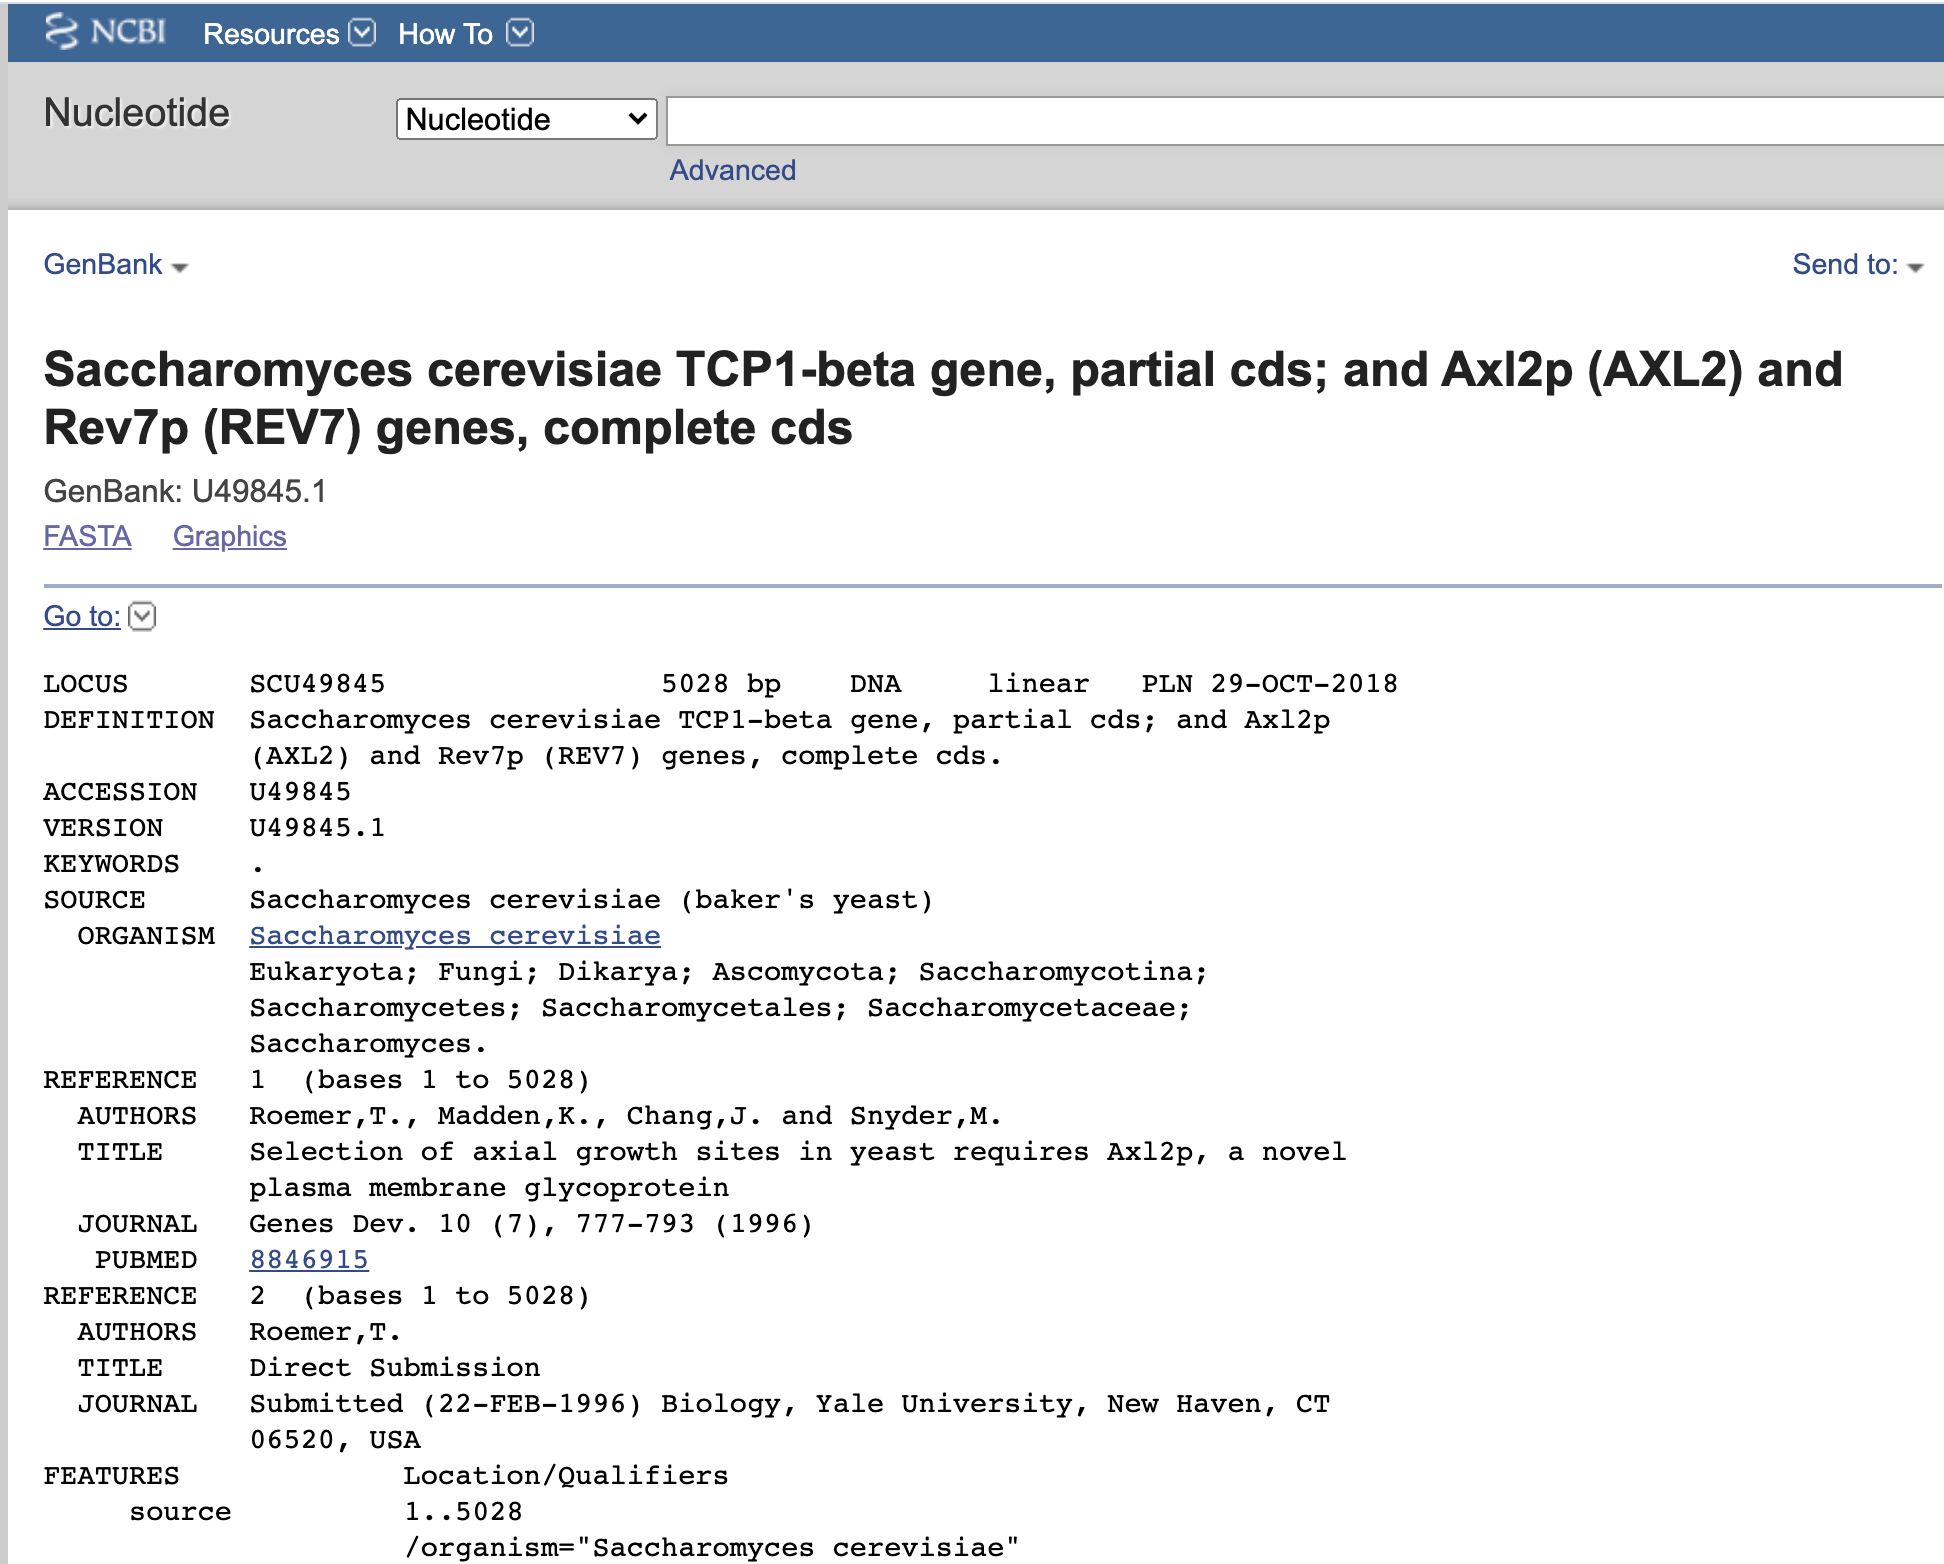
\includegraphics[width=27in]{images/genbank_record}

\hypertarget{pubmed-and-pubmed-central-article-database}{%
\section{PubMed and PubMed Central article database}\label{pubmed-and-pubmed-central-article-database}}

\textbf{PubMed} and \textbf{PubMed Central (PMC)} are databases of scientific articles related to data contained in NCBI databases. PubMed contains basic bibliographic information, the abstract, relevant links to sequences, and to the websites of the actual publishers of the papers. If the text of an article is open-access, PMC should have a copy of it. Articles in PMC contain relevant hyperlinks, such as to any sequences that are mentioned. For example, the image below show where the sequence of Tp0751 is mentioned in a paper and linked to the GenBank record we looked at above.

\hypertarget{entrez}{%
\section{Entrez}\label{entrez}}

\url{https://en.wikipedia.org/wiki/Entrez}

``Entrez is a federated search engine and web portal that allows users to search many discrete health sciences databases of the NCBI website. The name''Entrez'' (a greeting meaning ``Come in'' in French) was chosen to reflect the spirit of welcoming the public to search the content available from NCBI.''

``Entrez Global Query is an integrated search and retrieval system that provides access to all databases simultaneously with a single query and user interface. Entrez can efficiently retrieve related sequences, structures, and references. The Entrez system can provide views of gene and protein sequences and chromosome maps. Some textbooks are also available online through the Entrez system.''

\hypertarget{blast}{%
\section{BLAST}\label{blast}}

\url{https://en.wikipedia.org/wiki/BLAST_(biotechnology)}

``BLAST (basic local alignment search tool)is an algorithm and program for comparing primary biological sequence information, such as the amino-acid sequences of proteins or the nucleotides of DNA and/or RNA sequences. A BLAST search enables a researcher to compare a subject protein or nucleotide sequence (called a query) with a library or database of sequences, and identify database sequences that resemble the query sequence above a certain threshold. For example, following the discovery of a previously unknown gene in the mouse, a scientist will typically perform a BLAST search of the human genome to see if humans carry a similar gene; BLAST will identify sequences in the human genome that resemble the mouse gene based on similarity of sequence.''

\hypertarget{introduction-to-biological-sequences-databases}{%
\chapter{Introduction to biological sequences databases}\label{introduction-to-biological-sequences-databases}}

\begin{lstlisting}[language=R]
library(compbio4all)
\end{lstlisting}

\textbf{By}: Avril Coghlan.

\textbf{Adapted, edited and expanded}: Nathan Brouwer under the Creative Commons 3.0 Attribution License \href{https://creativecommons.org/licenses/by/3.0/}{(CC BY 3.0)}.

\hypertarget{topics}{%
\section{Topics}\label{topics}}

\begin{itemize}
\tightlist
\item
  NCBI vs.~EMBL vs.~DDBJ
\item
  annotation
\item
  Nucleotide vs.~Protein vs.~EST vs.~Genome
\item
  PubMed
\item
  GenBank Records
\item
  FASTA file format
\item
  FASTA header line
\item
  RefSeq
\item
  refining searches
\end{itemize}

\hypertarget{introduction}{%
\section{Introduction}\label{introduction}}

\textbf{NCBI} is the National Center for Biotechnology Information. The \href{www.ncbi.nlm.nih.gov/}{NCBI Webiste} is the entry point to a large number of databases giving access to \textbf{biological sequences} (DNA, RNA, protein) and biology-related publications.

When scientists sequence DNA, RNA and proteins they typically publish their data via databases with the NCBI. Each is given a unique identification number known as an \textbf{accession number}. For example, each time a unique human genome sequence is produced it is uploaded to the relevant databases, assigned a unique \textbf{accession}, and a website created to access it. Sequence are also cross-referenced to related papers, so you can start with a sequence and find out what scientific paper it was used in, or start with a paper and see if any sequences are associated with it.

This chapter provides an introduction to the general search features of the NCBI databases via the interface on the website, including how to locate sequences using accession numbers and other search parameters, such as specific authors or papers. Subsequent chapters will introduce advanced search features, and how to carry out searches using R commands.

One consequence of the explosion of biological sequences used in publications is that the system of databases has become fairly complex. There are databases for different types of data, different types of molecules, data from individual experiments showing \textbf{genetic variation} and also the \textbf{consensus sequence} for a given molecule. Luckily, if you know the accession number of the sequence you are looking for -- which will be our starting point throughout this book -- its fairly straight forward. There are numerous other books on bioinformatics and genomics that provide all details if you need to do more complex searches.

In this chapter we'll typically refer generically to ``NCBI data'' and ``NCBI databases.'' This is a simplification, since NCBI is the name of the organization and the databases and search engines often have specific names.

\hypertarget{biological-sequence-databases}{%
\section{Biological sequence databases}\label{biological-sequence-databases}}

Almost published biological sequences are available online, as it is a requirement of every scientific journal that any published DNA or RNA or protein sequence must be deposited in a public database. The main resources for storing and distributing sequence data are three large databases:

\begin{enumerate}
\def\labelenumi{\arabic{enumi}.}
\tightlist
\item
  USA: \textbf{\href{www.ncbi.nlm.nih.gov/}{NCBI database}} (www.ncbi.nlm.nih.gov/)
\item
  Europe: \textbf{European Molecular Biology Laboratory (EMBL)} database (\url{https://www.ebi.ac.uk/ena})
\item
  Japan: \textbf{DNA Database of Japan (DDBJ)} database (www.ddbj.nig.ac.jp/).
  These databases collect all publicly available DNA, RNA and protein sequence data and make it available for free. They exchange data nightly, so contain essentially the same data. The redundancy among the databases allows them to serve different communities (e.g.~native languages), provide different additional services such as tutorials, and assure that the world's scientists have their data backed up in different physical locations -- a key component of good data management!
\end{enumerate}

\hypertarget{the-ncbi-sequence-database}{%
\section{The NCBI Sequence Database}\label{the-ncbi-sequence-database}}

In this chapter we will explore the \textbf{NCBI sequence database} using the accession number NC\_001477, which is for the complete DEN-1 Dengue virus genome sequence. The accession number is reported in scientific papers originally describing the sequence, and also in subsequent papers that use that particular sequence.

In addition to the sequence itself, for each sequence the NCBI database also stores some additional \textbf{annotation} data, such as the name of the species it comes from, references to publications describing that sequence, information on the structure of the proteins coded by the sequence, etc. Some of this annotation data was added by the person who sequenced a sequence and submitted it to the NCBI database, while some may have been added later by a human curator working for NCBI.

\hypertarget{the-ncbi-sub-databases}{%
\section{The NCBI Sub-Databases}\label{the-ncbi-sub-databases}}

The NCBI database contains several sub-databases, the most important of which are:

\begin{itemize}
\tightlist
\item
  \textbf{Nucleotide database}: contains DNA and RNA sequences
\item
  \textbf{Protein database}: contains protein sequences
\item
  \textbf{EST database}: contains ESTs (expressed sequence tags), which are short sequences derived from mRNAs. (This terminology is likely to be unfamiliar because it is not often used in introductory biology courses. The ``Expressed'' of EST comes from the fact that mRNA is the result of gene expression.)
\item
  \textbf{Genome database}: contains the DNA sequences for entire genomes
\item
  \textbf{PubMed}: contains data on scientific publications
\end{itemize}

From the main NCBI website you can initiate a search and it will look for hits across all the databases. You can narrow your search by selecting a particular database.

\hypertarget{ncbi-genbank-record-format}{%
\section{NCBI GenBank Record Format}\label{ncbi-genbank-record-format}}

As mentioned above, for each sequence the NCBI database stores some extra information such as the species that it came from, publications describing the sequence, etc. This information is stored in the GenBank entry (aka GenBank Record) for the sequence. The GenBank entry for a sequence can be viewed by searching the NCBI database for the accession number for that sequence.

To view the GenBank entry for the DEN-1 Dengue virus, follow these steps:

\begin{enumerate}
\def\labelenumi{\arabic{enumi}.}
\tightlist
\item
  Go to the \href{www.ncbi.nlm.nih.gov}{NCBI website} (www.ncbi.nlm.nih.gov).
\item
  Search for the accession number NC\_001477.
\item
  Since we searched for a particular accession we are only returned a single main result which is titled ``NUCLEOTIDE SEQUENCE: Dengue virus 1, complete genome.''
\item
  Click on ``Dengue virus 1, complete genome'' to go to the GenBank entry.
\end{enumerate}

The GenBank entry for an accession contains a LOT of information about the sequence, such as papers describing it, features in the sequence, etc. The \textbf{DEFINITION} field gives a short description for the sequence. The \textbf{ORGANISM} field in the NCBI entry identifies the species that the sequence came from. The \textbf{REFERENCE} field contains scientific publications describing the sequence. The \textbf{FEATURES} field contains information about the location of features of interest inside the sequence, such as regulatory sequences or genes that lie inside the sequence. The \textbf{ORIGIN} field gives the sequence itself.

\hypertarget{the-fasta-file-format}{%
\section{The FASTA file format}\label{the-fasta-file-format}}

The \textbf{FASTA} file format is a simple file format commonly used to store and share sequence information. When you download sequences from databases such as NCBI you usually want FASTA files.

The first line of a FASTA file starts with the ``greater than'' character (\textgreater) followed by a name and/or description for the sequence. Subsequent lines contain the sequence itself. A short FASTA file might contain just something like this:

\begin{lstlisting}
## >mysequence1
## ACATGAGACAGACAGACCCCCAGAGACAGACCCCTAGACACAGAGAGAG
## TATGCAGGACAGGGTTTTTGCCCAGGGTGGCAGTATG
\end{lstlisting}

A FASTA file can contain the sequence for a single, an entire genome, or more than one sequence. If a FASTA file contains many sequences, then for each sequence it will have a \textbf{header line} starting with a greater than character followed by the sequence itself.

This is what a FASTA file with two sequence looks like.

\begin{lstlisting}
## >mysequence1
## ACATGAGACAGACAGACCCCCAGAGACAGACCCCTAGACACAGAGAGAG
## TATGCAGGACAGGGTTTTTGCCCAGGGTGGCAGTATG
## 
## >mysequence2
## AGGATTGAGGTATGGGTATGTTCCCGATTGAGTAGCCAGTATGAGCCAG
## AGTTTTTTACAAGTATTTTTCCCAGTAGCCAGAGAGAGAGTCACCCAGT
## ACAGAGAGC
\end{lstlisting}

\hypertarget{refseq}{%
\section{RefSeq}\label{refseq}}

When carrying out searches of the NCBI database, it is important to bear in mind that the database may contain \textbf{redundant sequences} for the same gene that were sequenced by different laboratories and experimental. This is because many different labs have sequenced the gene, and submitted their sequences to the NCBI database, and variation exists between individual organisms due to population-level variation due to previous mutations and also potential recent spontaneous mutations. There also can be some error in the sequencing process that results in differences between sequences.

There are also many different types of nucleotide sequences and protein sequences in the NCBI database. With respect to nucleotide sequences, some many be entire genomic DNA sequences, some may be mRNAs, and some may be lower quality sequences such as expressed sequence tags (ESTs, which are derived from parts of mRNAs), or DNA sequences of \textbf{contigs} from genome projects. That is, you can end up with an entry in the protein database based on sequence derived from a genomic sequence, from sequencing just the gene, and from other routes. Furthermore, some sequences may be \textbf{manually curated} by NCBI staff so that the associated entries contain extra information, but the majority of sequences are \textbf{uncurated.}

Therefore, NCBI databases often contains redundant information for a gene, contains sequences of varying quality, and contains both uncurated and curated data. As a result, NCBI has made a special database called \textbf{RefSeq (reference sequence database)}, which is a subset of the NCBI database. The data in RefSeq is manually curated, is high quality sequence data, and is non-redundant; this means that each gene (or \textbf{splice-form / isoform} of a gene, in the case of eukaryotes), protein, or genome sequence is only represented once.

The data in RefSeq is curated and is of much higher quality than the rest of the NCBI Sequence Database. However, unfortunately, because of the high level of manual curation required, RefSeq does not cover all species, and is not comprehensive for the species that are covered so far. To speed up searches and simplify the results in to can be very useful to just search RefSeq. However, for detailed and thorough work the full database should probably be searched and the results scrutinized.

You can easily tell that a sequence comes from RefSeq because its accession number starts with particular sequence of letters. That is, accessions of RefSeq sequences corresponding to protein records usually start with \textbf{NP\_}, and accessions of RefSeq curated complete genome sequences usually start with \textbf{NC\_} or \textbf{NS\_}.

\hypertarget{querying-the-ncbi-database}{%
\section{Querying the NCBI Database}\label{querying-the-ncbi-database}}

You may need to interrogate the NCBI Database to find particular sequences or a set of sequences matching given criteria, such as:

\begin{itemize}
\tightlist
\item
  The sequence with accession NC\_001477
\item
  The sequences published in Nature 460:352-358
\item
  All sequences from \emph{Chlamydia trachomatis}
\item
  Sequences submitted by Caroline Cameron, a syphilis researcher
\item
  Flagellin or fibrinogen sequences
\item
  The glutamine synthetase gene from \emph{Mycobacteriuma leprae}
\item
  Just the upstream control region of the \emph{Mycobacterium leprae} dnaA gene
\item
  The sequence of the \emph{Mycobacterium leprae} DnaA protein
\item
  The genome sequence of syphilis, \emph{Treponema pallidum} subspp. \emph{pallidum}
\item
  All human nucleotide sequences associated with malaria
\end{itemize}

There are two main ways that you can query the NCBI database to find these sets of sequences. The first possibility is to carry out searches on the NCBI website. The second possibility is to carry out searches from R using one of several packages that can interface with NCBI. As of October 2019 rentrez seems to be the best package for this..

Below, I will explain how to manually carry out queries on the NCBI database.

\hypertarget{querying-the-ncbi-database-via-the-ncbi-website-for-reference}{%
\section{Querying the NCBI Database via the NCBI Website (for reference)}\label{querying-the-ncbi-database-via-the-ncbi-website-for-reference}}

\textbf{NOTE}: The following section is here for reference; you need to know its \emph{possible} to refine searches but do not need to know any of these actual tags.

If you are carrying out searches on the NCBI website, to narrow down your searches to specific types of sequences or to specific organisms, you will need to use \textbf{``search tags''.}

For example, the search tags ``{[}PROP{]}'' and ``{[}ORGN{]}'' let you restrict your search to a specific subset of the NCBI Sequence Database, or to sequences from a particular taxon, respectively. Here is a list of useful search tags, which we will explain how to use below:

\begin{itemize}
\tightlist
\item
  {[}AC{]}, e.g.~NC\_001477{[}AC{]} With a particular accession number
\item
  {[}ORGN{]}, e.g.~Fungi{[}ORGN{]} From a particular organism or taxon
\item
  {[}PROP{]}, e.g.~biomol\_mRNA{[}PROP{]} Of a specific type (eg. mRNA) or from a specific database (eg. RefSeq)
\item
  {[}JOUR{]}, e.g.~Nature{[}JOUR{]} Described in a paper published in a particular journal
\item
  {[}VOL{]}, e.g.~531{[}VOL{]} Described in a paper published in a particular journal volume
\item
  {[}PAGE{]}, e.g.~27{[}PAGE{]} Described in a paper with a particular start-page in a journal
\item
  {[}AU{]}, e.g.~``Smith J''{[}AU{]} Described in a paper, or submitted to NCBI, by a particular author
\end{itemize}

To carry out searches of the NCBI database, you first need to go to the NCBI website, and type your search query into the search box at the top. For example, to search for all sequences from Fungi, you would type ``Fungi{[}ORGN{]}'' into the search box on the NCBI website.

You can combine the search tags above by using ``AND'', to make more complex searches. For example, to find all mRNA sequences from Fungi, you could type ``Fungi{[}ORGN{]} AND biomol\_mRNA{[}PROP{]}'' in the search box on the NCBI website.

Likewise, you can also combine search tags by using ``OR'', for example, to search for all mRNA sequences from Fungi or Bacteria, you would type ``(Fungi{[}ORGN{]} OR Bacteria{[}ORGN{]}) AND biomol\_mRNA{[}PROP{]}'' in the search box. Note that you need to put brackets around ``Fungi{[}ORGN{]} OR Bacteria{[}ORGN{]}'' to specify that the word ``OR'' refers to these two search tags.

Here are some examples of searches, some of them made by combining search terms using ``AND'':

\begin{itemize}
\tightlist
\item
  NC\_001477{[}AC{]} - With accession number NC\_001477
\item
  Nature{[}JOUR{]} AND 460{[}VOL{]} AND 352{[}PAGE{]} - Published in Nature 460:352-358
\item
  ``Chlamydia trachomatis''{[}ORGN{]} - From the bacterium Chlamydia trachomatis
\item
  ``Berriman M''{[}AU{]} - Published in a paper, or submitted to NCBI, by M. Berriman
\item
  flagellin OR fibrinogen - Which contain the word ``flagellin'' or ``fibrinogen'' in their NCBI record
\item
  ``Mycobacterium leprae''{[}ORGN{]} AND dnaA - Which are from M. leprae, and contain ``dnaA'' in their NCBI record
\item
  ``Homo sapiens''{[}ORGN{]} AND ``colon cancer'' - Which are from human, and contain ``colon cancer'' in their NCBI record
\item
  ``Homo sapiens''{[}ORGN{]} AND malaria - Which are from human, and contain ``malaria'' in their NCBI record
\item
  ``Homo sapiens''{[}ORGN{]} AND biomol\_mrna{[}PROP{]} - Which are mRNA sequences from human
\item
  ``Bacteria''{[}ORGN{]} AND srcdb\_refseq{[}PROP{]} - Which are RefSeq sequences from Bacteria
\item
  ``colon cancer'' AND srcdb\_refseq{[}PROP{]} - From RefSeq, which contain ``colon cancer'' in their NCBI record
\end{itemize}

Note that if you are searching for a phrase such as ``colon cancer'' or ``Chlamydia trachomatis'', you need to put the phrase in quotes when typing it into the search box. This is because if you type the phrase in the search box without quotes, the search will be for NCBI records that contain either of the two words ``colon'' or ``cancer'' (or either of the two words ``Chlamydia'' or ``trachomatis''), not necessarily both words.

As mentioned above, the NCBI database contains several sub-databases, including the NCBI \textbf{Nucleotide database} and the NCBI \textbf{Protein database}. If you go to the NCBI website, and type one of the search queries above in the search box at the top of the page, the results page will tell you how many matching NCBI records were found in each of the NCBI sub-databases.

For example, if you search for ``Chlamydia trachomatis{[}ORGN{]}'', you will get matches to proteins from C. trachomatis in the NCBI Protein database, matches to DNA and RNA sequences from \emph{C. trachomatis} in the NCBI Nucleotide database, matches to whole genome sequences for C. trachomatis strains in the NCBI Genome database, and so on:

Alternatively, if you know in advance that you want to search a particular sub-database, for example, the NCBI Protein database, when you go to the NCBI website, you can select that sub-database from the drop-down list above the search box, so that you will search that sub-database.

\hypertarget{example-finding-the-sequences-published-in-nature-460352-358-for-reference}{%
\section{Example: finding the sequences published in Nature 460:352-358 (for reference)}\label{example-finding-the-sequences-published-in-nature-460352-358-for-reference}}

\textbf{NOTE}: The following section is here for reference; you need to know its \emph{possible} to refine searches but do not need to know any of these actual tags.

For example, if you want to find sequences published in Nature 460:352-358, you can use the ``{[}JOUR{]}'', ``{[}VOL{]}'' and ``{[}PAGE{]}'' search terms. That is, you would go to the NCBI website and type in the search box on the top: ``Nature''{[}JOUR{]} AND 460{[}VOL{]} AND 352{[}PAGE{]}, where {[}JOUR{]} specifies the journal name, {[}VOL{]} the volume of the journal the paper is in, and {[}PAGE{]} the page number.

This should bring up a results page with ``50890'' beside the word ``Nucleotide'', and ``1'' beside the word ``Genome'', and ``25701'' beside the word ``Protein'', indicating that there were 50890 hits to sequence records in the Nucleotide database, which contains DNA and RNA sequences, and 1 hit to the Genome database, which contains genome sequences, and 25701 hits to the Protein database, which contains protein sequences.

If you click on the word ``Nucleotide'', it will bring up a webpage with a list of links to the NCBI sequence records for those 50890 hits. The 50890 hits are all contigs from the schistosome worm \emph{Schistosoma mansoni}.

Likewise, if you click on the word ``Protein'', it will bring up a webpage with a list of links to the NCBI sequence records for the 25701 hits, and you will see that the hits are all predicted proteins for \emph{Schistosoma mansoni}.

If you click on the word ``Genome'', it will bring you to the NCBI record for the \emph{Schistosoma mansoni} genome sequence, which has NCBI accession NS\_00200. Note that the accession starts with ``NS\_'', which indicates that it is a RefSeq accession.

Therefore, in Nature volume 460, page 352, the \emph{Schistosoma mansoni} genome sequence was published, along with all the DNA sequence contigs that were sequenced for the genome project, and all the predicted proteins for the gene predictions made in the genome sequence. You can view the original paper on the Nature website at \url{http://www.nature.com/nature/journal/v460/n7253/abs/nature08160.html}.

Note: \emph{Schistmosoma mansoni} is a parasitic worm that is responsible for causing \textbf{schistosomiasis}, which is classified by the WHO as a \textbf{neglected tropical disease}.

\hypertarget{downloading-ncbi-sequence-data-by-hand}{%
\chapter{Downloading NCBI sequence data by hand}\label{downloading-ncbi-sequence-data-by-hand}}

\textbf{By}: Avril Coghlan.

\textbf{Adapted, edited and expanded}: Nathan Brouwer under the Creative Commons 3.0 Attribution License \href{https://creativecommons.org/licenses/by/3.0/}{(CC BY 3.0)}.

\hypertarget{preface-3}{%
\section{Preface}\label{preface-3}}

The following chapter was originally written by Avril Coghlan. It provides brief, basic information for how to access sequences via the internet. Subsequent chapters provide more details and R code.

\hypertarget{retrieving-genome-sequence-data-via-the-ncbi-website}{%
\section{Retrieving genome sequence data via the NCBI website}\label{retrieving-genome-sequence-data-via-the-ncbi-website}}

You can easily retrieve DNA or protein sequence data by hand from the \href{www.ncbi.nlm.nih.gov}{NCBI} Sequence Database via its website www.ncbi.nlm.nih.gov.

Dengue DEN-1 DNA is a viral DNA sequence and its NCBI \textbf{accession number} is NC\_001477. To retrieve the DNA sequence for the Dengue DEN-1 virus from NCBI, go to the NCBI website, type ``NC\_001477'' in the Search box at the top of the webpage, and press the ``Search'' button beside the Search box.

(While this is the normal workflow, accessions related to well-known organisms can sometimes turn up using a direct Google search. This is the case for NC\_001477 - if you Google it you can go directly to the website with the genome sequence.)

On the results page of a normal NCBI search you will see the number of hits to ``NC\_001477'' in each of the NCBI databases on the NCBI website. There are \emph{many} databases on the NCBI website, for example, \textbf{PubMed} and \textbf{Pubmed Central} contain abstracts from scientific papers, the \textbf{Genes} and \textbf{Genomes} database contains DNA and RNA sequence data, the \textbf{Proteins} database contains protein sequence data, and so on.

Most biologist would do this type of work by hand from within their web browser, but it can also be done by writing small programs in \textbf{scripting languages} such as \textbf{Python} or \textbf{R}. In R, the \textbf{rentrez} package is a powerful tool for intersecting with NCBI resource. In this tutorial we'll focus on the web interface. Its good to remember, though, that almost anything done via the webpage can be automated using a computer \textbf{script}.

A challenge when learning to use NCBI resources is that there is a tremendous amount of sequence information available and you need to learn how to sort through what the search results provide. As you are looking for the \emph{DNA} sequence of the Dengue DEN-1 virus genome, you expect to see a hit in the NCBI \textbf{Nucleotide database}. This is indicated at the top of the page where it says ``\textbf{NUCLEOTIDE SEQUENCE}'' and lists ``Dengue virus 1, complete genome.''

When you click on the link for the Nucleotide database, it will bring you to the record for NC\_001477 in the NCBI Nucleotide database. This will contain the name and NCBI \textbf{accession} of the sequence, as well as other details such as any papers describing the sequence. If you scroll down you'll see the sequence also.

If you need it, you can retrieve the DNA sequence for the DEN-1 Dengue virus genome sequence as a \textbf{FASTA format} sequence file in a couple ways. The easiest is just to copy and paste it into a text, .R, or other file. You can also click on \textbf{``Send to''} at the top right of the NC\_001477 sequence record webpage (just to the left of the side bar; its kinda small).

After you click on \textbf{Send to} you can pick several options. and then choose ``File'' in the menu that appears, and then choose FASTA from the ``Format'' menu that appears, and click on ``Create file''. The sequence will then download. The default file name is \textbf{sequence.fasta} so you'll probably want to change it.

You can now open the FASTA file containing the DEN-1 Dengue virus genome sequence using a text editor like Notepad, WordPad, Notepad++, or even RStudio on your computer. To find a text editor on your computer search for ``text'' from the start menu (Windows) and usually one will come up. (Opening the file in a word processor like word isn't recommended).

\hypertarget{downloading-sequences-from-uniprot-by-hand}{%
\chapter{Downloading sequences from UniProt by hand}\label{downloading-sequences-from-uniprot-by-hand}}

\textbf{By}: Avril Coghlan.

\textbf{Adapted, edited and expanded}: Nathan Brouwer under the Creative Commons 3.0 Attribution License \href{https://creativecommons.org/licenses/by/3.0/}{(CC BY 3.0)}.

\hypertarget{vocab-1}{%
\section{Vocab}\label{vocab-1}}

\begin{itemize}
\tightlist
\item
  RefSeq
\item
  manual curation
\item
  UniProt
\item
  accession
\end{itemize}

\hypertarget{downloading-protein-data-from-uniprot}{%
\section{Downloading Protein data from UniProt}\label{downloading-protein-data-from-uniprot}}

In a previous vignette you learned how to retrieve sequences from the NCBI database. The NCBI database is a key database in bioinformatics because it contains essentially all DNA sequences ever sequenced.

As mentioned previously, a subsection of the NCBI database called \textbf{RefSeq} consists of high quality DNA and protein sequence data. Furthermore, the NCBI entries for the RefSeq sequences have been \textbf{manually curated}, which means that expert biologists employed by NCBI have added additional information to the NCBI entries for those sequences, such as details of scientific papers that describe the sequences.

Another extremely important manually curated database is \href{www.uniprot.org}{\textbf{UniProt}}, which focuses on protein sequences. UniProt aims to contains manually curated information on all known protein sequences. While many of the protein sequences in UniProt are also present in RefSeq, the amount and quality of manually curated information in UniProt is much higher than that in RefSeq.

For each protein in UniProt, the UniProt curators read all the scientific papers that they can find about that protein, and add information from those papers to the protein's UniProt entry. For example, for a human protein, the UniProt entry for the protein usually includes information about the biological function of the protein, in what human tissues it is expressed, whether it interacts with other human proteins, and much more. All this information has been manually gathered by the UniProt curators from scientific papers, and the papers in which the found the information are always listed in the UniProt entry for the protein.

Just like NCBI, UniProt also assigns an \textbf{accession} to each sequence in the UniProt database. Although the same protein sequence may appear in both the NCBI database and the UniProt database, it will have \emph{different} NCBI and UniProt accessions. However, there is usually a link on the NCBI entry for the protein sequence to the UniProt entry, and vice versa.

\hypertarget{viewing-the-uniprot-webpage-for-a-protein-sequence}{%
\section{Viewing the UniProt webpage for a protein sequence}\label{viewing-the-uniprot-webpage-for-a-protein-sequence}}

If you are given the UniProt accession for a protein, to find the UniProt entry for the protein, you first need to go the UniProt website, www.uniprot.org. At the top of the UniProt website, you will see a search box, and you can type the accession of the protein that you are looking for in this search box, and then click on the ``Search'' button to search for it.

For example, if you want to find the sequence for the chorismate lyase protein from \emph{Mycobacterium leprae} (the bacterium which causes leprosy), which has UniProt accession Q9CD83, you would type just ``Q9CD83'' in the search box and press ``Search''. The UniProt entry for UniProt accession Q9CD83 will then appear in your web browser.

Beside the heading ``Organism'' you can see the organism is given as \emph{Mycobacterium leprae}. If you scroll down you'll find a section \textbf{Names and Taxonomy} and beside the heading ``Taxonomic lineage'', you can see ``Bacteria - Actinobacteria - Actinobacteridae - Actinomycetales - Corynebacterineae - Mycobacteriaceae- Mycobacterium''.

This tells us that \emph{Mycobacterium} is a species of bacteria, which belongs to a group of related bacteria called the Mycobacteriaceae, which itself belongs to a larger group of related bacteria called the Corynebacterineae, which itself belongs to an even larger group of related bacteria called the Actinomycetales, which itself belongs to the Actinobacteridae, which itself belongs to a huge group of bacteria called the Actinobacteria.

\hypertarget{protein-function}{%
\subsection{Protein function}\label{protein-function}}

Back up at the top under ``organism'' is says ``Status'', which tells us the \textbf{annotation score} is 2 out of 5, that it is a ``Protein inferred from homology'', which means what we know about it is derived from bioinformatics and computational tools, not lab work.

Beside the heading ``Function'', it says that the function of this protein is that it ``Removes the pyruvyl group from chorismate to provide 4-hydroxybenzoate (4HB)''. This tells us this protein is an enzyme (a protein that increases the rate of a specific biochemical reaction), and tells us what is the particular biochemical reaction that this enzyme is involved in. At the end of this info it says ``By similarity'', which again indicates that what we know about this protein comes from bioinformatics, not lab work.

\hypertarget{protein-sequence-and-size}{%
\subsection{Protein sequence and size}\label{protein-sequence-and-size}}

Under \textbf{Sequence} we see that the sequence length is 210 amino acids long (210 letters long) and has a mass of 24,045 daltons. We can access the sequence as a FASTA file from here if we want and also carry out a BLAST search from a link on the right.

\hypertarget{other-information}{%
\subsection{Other information}\label{other-information}}

Further down the UniProt page for this protein, you will see a lot more information, as well as many links to webpages in other biological databases, such as NCBI. The huge amount of information about proteins in UniProt means that if you want to find out about a particular protein, the UniProt page for that protein is a great place to start.

\hypertarget{retrieving-a-uniprot-protein-sequence-via-the-uniprot-website}{%
\section{Retrieving a UniProt protein sequence via the UniProt website}\label{retrieving-a-uniprot-protein-sequence-via-the-uniprot-website}}

There are a couple different ways to retrieve the sequence. At the top of the page is a tab that say ``Format'' which brings you to a page with th FASTA file. You can copy and paste the sequence from here if you want. To save it as a file, go to the ``File'' menu of your web browser, choose ``Save page as'', and save the file. Remember to give the file a sensible name (eg. ``Q9CD83.fasta'' for accession Q9CD83), and in a place that you will remember (eg. in the ``My Documents'' folder).

For example, you can retrieve the protein sequences for the chorismate lyase protein from \emph{Mycobacterium leprae} (which has UniProt accession Q9CD83) and for the chorismate lyase protein from \emph{Mycobacterium ulcerans} (UniProt accession A0PQ23), and save them as FASTA-format files (eg. ``Q9CD83.fasta'' and ``A0PQ23.fasta'', as described above.

You can also put the UniProt information into an online \textbf{Basket}. If you do this for both Q9CD83 and A0PQ23 you can think click on \textbf{Basket}, select both entries, and carry out a pairwise alignment by clicking on \textbf{Align}.

\emph{Mycobacterium leprae} is the bacterium which causes leprosy, while \emph{Mycobacterium ulcerans} is a related bacterium which causes Buruli ulcer, both of which are classified by the WHO as neglected tropical diseases. The \emph{M. leprae} and \emph{M. ulcerans} chorismate lyase proteins are an example of a pair of \textbf{homologous} (related) proteins in two related species of bacteria.

If you downloaded the protein sequences for UniProt accessions Q9CD83 and A0PQ23 and saved them as FASTA-format files (eg. ``Q9CD83.fasta'' and ``A0PQ23.fasta''), you could read them into R using the read.fasta() function in the SeqinR R package (as detailed in another Vignette) or a similar function from another package.

Note that the read.fasta() function normally expects that you have put your FASTA-format files in the the \textbf{working directory} of R. For convenience so you can explore these sequences they have been saved in a special folder in the \emph{compbio4all} package and can be accessed like this for the Leprosy sequence

\begin{lstlisting}[language=R]
# load compbio4all
library(compbio4all)

# locate the file within the package using system.file()
file.1 <- system.file("./extdata/Q9CD83.fasta",package = "compbio4all")

# load seqinr
library("seqinr")

# load fasta
leprae <- read.fasta(file = file.1)
lepraeseq <- leprae[[1]]
\end{lstlisting}

We can confirm

\begin{lstlisting}[language=R]
str(lepraeseq)
\end{lstlisting}

For the other sequence

\begin{lstlisting}[language=R]
# locate the file within the package using system.file()
file.2 <- system.file("./extdata/A0PQ23.fasta", package = "compbio4all")


# load fasta
ulcerans <- read.fasta(file = file.2)
ulceransseq <- ulcerans[[1]]
\end{lstlisting}

\hypertarget{introducingFASTA}{%
\chapter{Introducing FASTA Files}\label{introducingFASTA}}

Adapted from \href{https://en.wikipedia.org/wiki/FASTA_format}{Wikipedia}: \url{https://en.wikipedia.org/wiki/FASTA_format}

In bioinformatics, the FASTA format is a text-based format for representing either nucleotide sequences or amino acid (protein) sequences, in which nucleotides or amino acids are represented using single-letter codes. The format allows for sequence names and comments to precede the sequences. The format originates from the FASTA alignment software, but has now become a near universal standard in the field of bioinformatics.

The simplicity of FASTA format makes it easy to manipulate and parse sequences using text-processing tools and scripting languages like the R programming language and Python.

The first line in a FASTA file starts with a ``\textgreater{}'' (greater-than) symbol and holds summary information about the sequence, often starting with a unique accession number and followed by information like the name of the gene, the type of sequence, and the organism it is from.

On the next is the sequence itself in a standard one-letter character string. Anything other than a valid character is be ignored (including spaces, tabs, asterisks, etc\ldots).

A multiple sequence FASTA format can be obtained by concatenating several single sequence FASTA files in a common file (also known as multi-FASTA format).

Following the header line, the actual sequence is represented. Sequences may be protein sequences or nucleic acid sequences, and they can contain gaps or alignment characters. Sequences are expected to be represented in the standard amino acid and nucleic acid codes. Lower-case letters are accepted and are mapped into upper-case; a single hyphen or dash can be used to represent a gap character; and in amino acid sequences, U and * are acceptable letters.

FASTQ format is a form of FASTA format extended to indicate information related to sequencing. It is created by the Sanger Centre in Cambridge.

Bioconductor.org's Biostrings package can be used to read and manipulate FASTA files in R

\begin{quote}
``FASTA format is a text-based format for representing either nucleotide sequences or peptide sequences, in which base pairs or amino acids are represented using single-letter codes. A sequence in FASTA format begins with a single-line description, followed by lines of sequence data. The description line is distinguished from the sequence data by a greater-than (''\textgreater{}``) symbol in the first column. It is recommended that all lines of text be shorter than 80 characters in length.'' (\url{https://zhanglab.dcmb.med.umich.edu/FASTA/})
\end{quote}

\hypertarget{example-fasta-file}{%
\section{Example FASTA file}\label{example-fasta-file}}

Here is an example of the contents of a FASTA file. (If your are viewing this chapter in the form of the source .Rmd file, the \passthrough{\lstinline!cat()!} function is included just to print out the content properly and is not part of the FASTA format).

\begin{lstlisting}[language=R]
cat(">gi|186681228|ref|YP_001864424.1| phycoerythrobilin:ferredoxin oxidoreductase
MNSERSDVTLYQPFLDYAIAYMRSRLDLEPYPIPTGFESNSAVVGKGKNQEEVVTTSYAFQTAKLRQIRA
AHVQGGNSLQVLNFVIFPHLNYDLPFFGADLVTLPGGHLIALDMQPLFRDDSAYQAKYTEPILPIFHAHQ
QHLSWGGDFPEEAQPFFSPAFLWTRPQETAVVETQVFAAFKDYLKAYLDFVEQAEAVTDSQNLVAIKQAQ
LRYLRYRAEKDPARGMFKRFYGAEWTEEYIHGFLFDLERKLTVVK")
\end{lstlisting}

\begin{lstlisting}
## >gi|186681228|ref|YP_001864424.1| phycoerythrobilin:ferredoxin oxidoreductase
## MNSERSDVTLYQPFLDYAIAYMRSRLDLEPYPIPTGFESNSAVVGKGKNQEEVVTTSYAFQTAKLRQIRA
## AHVQGGNSLQVLNFVIFPHLNYDLPFFGADLVTLPGGHLIALDMQPLFRDDSAYQAKYTEPILPIFHAHQ
## QHLSWGGDFPEEAQPFFSPAFLWTRPQETAVVETQVFAAFKDYLKAYLDFVEQAEAVTDSQNLVAIKQAQ
## LRYLRYRAEKDPARGMFKRFYGAEWTEEYIHGFLFDLERKLTVVK
\end{lstlisting}

\hypertarget{multiple-sequences-in-a-single-fasta-file}{%
\section{Multiple sequences in a single FASTA file}\label{multiple-sequences-in-a-single-fasta-file}}

Multiple sequences can be stored in a single FASTA file, each on separated by a line and have its own headline.

\begin{lstlisting}[language=R]
cat(">LCBO - Prolactin precursor - Bovine
MDSKGSSQKGSRLLLLLVVSNLLLCQGVVSTPVCPNGPGNCQVSLRDLFDRAVMVSHYIHDLSS
EMFNEFDKRYAQGKGFITMALNSCHTSSLPTPEDKEQAQQTHHEVLMSLILGLLRSWNDPLYHL
VTEVRGMKGAPDAILSRAIEIEEENKRLLEGMEMIFGQVIPGAKETEPYPVWSGLPSLQTKDED
ARYSAFYNLLHCLRRDSSKIDTYLKLLNCRIIYNNNC*

>MCHU - Calmodulin - Human, rabbit, bovine, rat, and chicken
MADQLTEEQIAEFKEAFSLFDKDGDGTITTKELGTVMRSLGQNPTEAELQDMINEVDADGNGTID
FPEFLTMMARKMKDTDSEEEIREAFRVFDKDGNGYISAAELRHVMTNLGEKLTDEEVDEMIREA
DIDGDGQVNYEEFVQMMTAK*

>gi|5524211|gb|AAD44166.1| cytochrome b [Elephas maximus maximus]
LCLYTHIGRNIYYGSYLYSETWNTGIMLLLITMATAFMGYVLPWGQMSFWGATVITNLFSAIPYIGTNLV
EWIWGGFSVDKATLNRFFAFHFILPFTMVALAGVHLTFLHETGSNNPLGLTSDSDKIPFHPYYTIKDFLG
LLILILLLLLLALLSPDMLGDPDNHMPADPLNTPLHIKPEWYFLFAYAILRSVPNKLGGVLALFLSIVIL
GLMPFLHTSKHRSMMLRPLSQALFWTLTMDLLTLTWIGSQPVEYPYTIIGQMASILYFSIILAFLPIAGX
IENY")
\end{lstlisting}

\begin{lstlisting}
## >LCBO - Prolactin precursor - Bovine
## MDSKGSSQKGSRLLLLLVVSNLLLCQGVVSTPVCPNGPGNCQVSLRDLFDRAVMVSHYIHDLSS
## EMFNEFDKRYAQGKGFITMALNSCHTSSLPTPEDKEQAQQTHHEVLMSLILGLLRSWNDPLYHL
## VTEVRGMKGAPDAILSRAIEIEEENKRLLEGMEMIFGQVIPGAKETEPYPVWSGLPSLQTKDED
## ARYSAFYNLLHCLRRDSSKIDTYLKLLNCRIIYNNNC*
## 
## >MCHU - Calmodulin - Human, rabbit, bovine, rat, and chicken
## MADQLTEEQIAEFKEAFSLFDKDGDGTITTKELGTVMRSLGQNPTEAELQDMINEVDADGNGTID
## FPEFLTMMARKMKDTDSEEEIREAFRVFDKDGNGYISAAELRHVMTNLGEKLTDEEVDEMIREA
## DIDGDGQVNYEEFVQMMTAK*
## 
## >gi|5524211|gb|AAD44166.1| cytochrome b [Elephas maximus maximus]
## LCLYTHIGRNIYYGSYLYSETWNTGIMLLLITMATAFMGYVLPWGQMSFWGATVITNLFSAIPYIGTNLV
## EWIWGGFSVDKATLNRFFAFHFILPFTMVALAGVHLTFLHETGSNNPLGLTSDSDKIPFHPYYTIKDFLG
## LLILILLLLLLALLSPDMLGDPDNHMPADPLNTPLHIKPEWYFLFAYAILRSVPNKLGGVLALFLSIVIL
## GLMPFLHTSKHRSMMLRPLSQALFWTLTMDLLTLTWIGSQPVEYPYTIIGQMASILYFSIILAFLPIAGX
## IENY
\end{lstlisting}

\hypertarget{multiple-sequence-alignments-can-be-stored-in-fasta-format}{%
\section{Multiple sequence alignments can be stored in FASTA format}\label{multiple-sequence-alignments-can-be-stored-in-fasta-format}}

\textbf{Aligned FASTA format} can be used to store the output of \textbf{Multiple Sequence Alignment (MSA)}. This format contains

\begin{enumerate}
\def\labelenumi{\arabic{enumi}.}
\tightlist
\item
  Multiple entries, each with their own header line
\item
  \textbf{Gaps} inserted to align sequences are indicated by \passthrough{\lstinline!.!}
\item
  Each spaces added to the beginning and end of sequences that vary in length are indicated by \passthrough{\lstinline!\~!}
\end{enumerate}

In the sample FASTA file below, the \passthrough{\lstinline!example1!} sequence has a gap of 8 near its beginning. The \passthrough{\lstinline!example2!} sequence has numerous \passthrough{\lstinline!\~!} indicating that this sequence is missing data from its beginning that are present in the other sequences. The \passthrough{\lstinline!example3!} sequence has numerous \passthrough{\lstinline!\~!} at its end, indicating that this sequence is shorter than the others.

\begin{lstlisting}[language=R]
cat(">example1 
MKALWALLLVPLLTGCLA........EGELEVTDQLPGQSDQP.WEQALNRFWDYLRWVQ
GNQARDRLEEVREQMEEVRSKMEEQTQQIRLQAEIFQARIKGWFEPLVEDMQRQWANLME
KIQASVATNSIASTTVPLENQ
>example2 
~~~~~~~~~~~~~~~~~~~~~~~~~~KVQQELEPEAGWQTGQP.WEAALARFWDYLRWVQ
SSRARGHLEEMREQIQEVRVKMEEQADQIRQKAEAFQARLKSWFEPLLEDMQRQWDGLVE
KVQAAVAT.IPTSKPVEEP~~
>example3 
MRSLVVFFALAVLTGCQARSLFQAD..............APQPRWEEMVDRFWQYVSELN
AGALKEKLEETAENL...RTSLEGRVDELTSLLAPYSQKIREQLQEVMDKIKEATAALPT
QA~~~~~~~~~~~~~~~~~~~")
\end{lstlisting}

\begin{lstlisting}
## >example1 
## MKALWALLLVPLLTGCLA........EGELEVTDQLPGQSDQP.WEQALNRFWDYLRWVQ
## GNQARDRLEEVREQMEEVRSKMEEQTQQIRLQAEIFQARIKGWFEPLVEDMQRQWANLME
## KIQASVATNSIASTTVPLENQ
## >example2 
## ~~~~~~~~~~~~~~~~~~~~~~~~~~KVQQELEPEAGWQTGQP.WEAALARFWDYLRWVQ
## SSRARGHLEEMREQIQEVRVKMEEQADQIRQKAEAFQARLKSWFEPLLEDMQRQWDGLVE
## KVQAAVAT.IPTSKPVEEP~~
## >example3 
## MRSLVVFFALAVLTGCQARSLFQAD..............APQPRWEEMVDRFWQYVSELN
## AGALKEKLEETAENL...RTSLEGRVDELTSLLAPYSQKIREQLQEVMDKIKEATAALPT
## QA~~~~~~~~~~~~~~~~~~~
\end{lstlisting}

\hypertarget{fastq-format}{%
\section{FASTQ Format}\label{fastq-format}}

Adapted from \href{https://en.wikipedia.org/wiki/FASTQ_format}{Wikipedia}: \url{https://en.wikipedia.org/wiki/FASTQ_format}

FASTQ format is a text-based format for storing both a biological sequence (usually nucleotide sequence) and its corresponding quality scores. Both the sequence letter and quality score are each encoded with a single ASCII character for brevity.

It was originally developed at the Wellcome Trust Sanger Institute to bundle a FASTA formatted sequence and its quality data, but has recently become the de facto standard for storing the output of high-throughput sequencing instruments such as the Illumina Genome Analyzer.

A FASTQ file normally uses four lines per sequence.

\begin{itemize}
\tightlist
\item
  Line 1 begins with a \passthrough{\lstinline!@!} character and is followed by a sequence identifier and an optional description (like a FASTA title line).
\item
  Line 2 is the raw sequence letters.
\item
  Line 3 begins with a \passthrough{\lstinline!+!} character and is optionally followed by the same sequence identifier (and any description) again.
\item
  Line 4 encodes the \textbf{quality values} for the sequence in Line 2 of the file, and must contain the same number of symbols as letters in the sequence.
\end{itemize}

A FASTQ file containing a single sequence might look like this:''

\begin{lstlisting}[language=R]
cat("@SEQ_ID
GATTTGGGGTTCAAAGCAGTATCGATCAAATAGTAAATCCATTTGTTCAACTCACAGTTT
+
!''*((((***+))%%%++)(%%%%).1***-+*''))**55CCF>>>>>>CCCCCCC65")
\end{lstlisting}

\begin{lstlisting}
## @SEQ_ID
## GATTTGGGGTTCAAAGCAGTATCGATCAAATAGTAAATCCATTTGTTCAACTCACAGTTT
## +
## !''*((((***+))%%%++)(%%%%).1***-+*''))**55CCF>>>>>>CCCCCCC65
\end{lstlisting}

Here are the quality value characters in left-to-right increasing order of quality (ASCII):''

\begin{lstlisting}[language=R]
 !"#$%&'()*+,-./0123456789:;<=>?@ABCDEFGHIJKLMNOPQRSTUVWXYZ[\]^_`abcdefghijklmnopqrstuvwxyz{|}~
\end{lstlisting}

FASTQ files typically do not include line breaks and do not wrap around when they reach the width of a normal page or file.

\hypertarget{a-complete-bioinformatics-workflow-in-r}{%
\chapter{A complete bioinformatics workflow in R}\label{a-complete-bioinformatics-workflow-in-r}}

\textbf{By}: Nathan L. Brouwer

\hypertarget{worked-example-building-a-phylogeny-in-r}{%
\chapter{``Worked example: Building a phylogeny in R''}\label{worked-example-building-a-phylogeny-in-r}}

\hypertarget{introduction-1}{%
\section{Introduction}\label{introduction-1}}

Phylogenies play an important role in computational biology and bioinformatics. Phylogenetics itself is an obligatly computational field that only began rapid growth when computational power allowed the many algorithms it relies on to be done rapidly. Phylogeneies of species, genes and proteins are used to address many biological issues, including

\begin{itemize}
\tightlist
\item
  Patterns of protein evolution
\item
  Origin and evolution of phenotypic traits
\item
  Origin and progression of epidemics
\item
  Origin of evolution of diseases (eg, zooenoses)
\item
  Prediction of protein function from its sequence
\item
  \ldots{} and many more
\end{itemize}

The actual building of a phylogeny is a computationally intensive task; moreover, there are many bioinformatics and computational tasks the precede the construction of a phylogeny:

\begin{itemize}
\tightlist
\item
  genome sequencing and assembly
\item
  computational gene prediction and annotation
\item
  database searching and results screening
\item
  pairwise sequence alignment
\item
  data organization and cleaning
\item
  multiple sequence alignment
\item
  evaluation and validation of alignment accuracy
\end{itemize}

Once all of these steps have been carried out, the building of a phylogeny involves

\begin{itemize}
\tightlist
\item
  picking a model of sequence evolution or other description of evolution
\item
  picking a statistical approach to tree construction
\item
  evaluating uncertainty in the final tree
\end{itemize}

In this chapter we will work through many of these steps. In most cases we will pick the easiest or fastest option; in later chapters we will unpack the various options. This chapter is written as an interactive R sessions. You can follow along by opening the .Rmd file of the chapter or typing the appropriate commands into your own script. I assume that all the necessary packages have been installed and they only need to be loaded into R using the \emph{library()} command.

This lesson walks you through and entire workflow for a bioinformatics, including

\begin{enumerate}
\def\labelenumi{\arabic{enumi}.}
\tightlist
\item
  obtaining FASTA sequences
\item
  cleaning sequences
\item
  creating alignments
\item
  creating distance a distance matrix
\item
  building a phylogenetic tree
\end{enumerate}

We'll examine the Shroom family of genes, which produces Shroom proteins essential for tissue formation in many multicellular eukaryotes, including neural tube formation in vertebrates. We'll examine shroom in several very different organism, including humans, mice and sea urchins. There is more than one type of shroom in vertebrates, and we'll also look at two different Shroom genes: shroom 1 and shroom 2.

This lesson draws on skills from previous sections of the book, but is written to act as a independent summary of these activities. There is therefore review of key aspects of R and bioinformatics throughout it.

\hypertarget{software-preliminaires}{%
\section{Software Preliminaires}\label{software-preliminaires}}

\hypertarget{vocab-2}{%
\subsection{Vocab}\label{vocab-2}}

\begin{itemize}
\tightlist
\item
  argument
\item
  function
\item
  list
\item
  named list
\item
  vector
\item
  named vector
\item
  for() loop
\item
  R console
\end{itemize}

\hypertarget{r-functions-1}{%
\subsection{R functions}\label{r-functions-1}}

\begin{itemize}
\tightlist
\item
  library()
\item
  round()
\item
  plot()
\item
  mtext()
\item
  nchar()
\item
  rentrez::entrez\_fetch()
\item
  compbio4all::entrez\_fetch\_list()
\item
  compbio4all::print\_msa() (Coghlan 2011)
\item
  Biostrings::AAStringSet()
\item
  msa::msa()
\item
  msa::msaConvert()
\item
  msa::msaPrettyPrint()
\item
  seqinr::dist.alignment()
\item
  ape::nj()
\end{itemize}

A few things need to be done to get started with our R session.

\hypertarget{download-necessary-packages}{%
\subsection{Download necessary packages}\label{download-necessary-packages}}

Many \emph{R} sessions begin by downloading necessary software packages to augment \emph{R's} functionality.

If you don't have them already, you'll need the following packages from CRAN:

\begin{enumerate}
\def\labelenumi{\arabic{enumi}.}
\tightlist
\item
  \passthrough{\lstinline!ape!}
\item
  \passthrough{\lstinline!seqinr!}
\item
  \passthrough{\lstinline!rentrez!}
\item
  \passthrough{\lstinline!devtools!}
\end{enumerate}

The CRAN packages can be loaded with \passthrough{\lstinline!install.packages()!}.

You'll also need these packages from Bioconductor:

\begin{enumerate}
\def\labelenumi{\arabic{enumi}.}
\tightlist
\item
  \passthrough{\lstinline!msa!}
\item
  \passthrough{\lstinline!Biostrings!}
\end{enumerate}

For installing packages from Bioconductor, see the chapter at the beginning of this book on this process.

Finally, you'll need this package from GitHub

\begin{enumerate}
\def\labelenumi{\arabic{enumi}.}
\tightlist
\item
  \passthrough{\lstinline!compbio4all!}
\item
  \passthrough{\lstinline!ggmsa!}
\end{enumerate}

To install packages from GitHub you can use the code \passthrough{\lstinline!devtools::install\_github("brouwern/combio4all")!} and \passthrough{\lstinline!devtools::install\_github("brouwern/ggmsa")!}

\hypertarget{load-packages-into-memory}{%
\subsection{Load packages into memory}\label{load-packages-into-memory}}

We now need to load up all our bioinformatics and phylogenetics software into R. This is done with the \passthrough{\lstinline!library()!} command.

To run this code just clock on the sideways green triangle all the way to the right of the code.

NOTE: You'll likely see some red code appear on your screen. No worries, totally normal!

\begin{lstlisting}[language=R]
# github packages
library(compbio4all)

# CRAN packages
library(rentrez)
library(seqinr)
library(ape)

# Bioconductor packages
library(msa)
library(Biostrings)
\end{lstlisting}

\hypertarget{downloading-macro-molecular-sequences}{%
\section{Downloading macro-molecular sequences}\label{downloading-macro-molecular-sequences}}

We're going to explore some sequences. First we need to download them. To do this we'll use a function, \passthrough{\lstinline!entrez\_fretch()!}, which accesses the \href{ncbi.nlm.nih.gov/search/}{\textbf{Entrez}} system of database (ncbi.nlm.nih.gov/search/). This function is from the \passthrough{\lstinline!rentrez!} package, which stands for ``R-Entrez.''

We need to tell \passthrough{\lstinline!entrez\_fetch()!} several things

\begin{enumerate}
\def\labelenumi{\arabic{enumi}.}
\tightlist
\item
  \passthrough{\lstinline!db = ...!} the type of entrez database.\\
\item
  \passthrough{\lstinline!id = ...!} the \textbf{accession} (ID) number of the sequence
\item
  \passthrough{\lstinline!rettype = ...!} file type what we want the function to return.
\end{enumerate}

Formally, these things are called \textbf{arguments} by \emph{R}.

We'll use these settings:

\begin{enumerate}
\def\labelenumi{\arabic{enumi}.}
\tightlist
\item
  \passthrough{\lstinline!db = "protein"!} to access the Entrez database of protein sequences\\
\item
  \passthrough{\lstinline!rettype = "fasta"!}, which is a standard file format for nucleic acid and protein sequences
\end{enumerate}

We'll set \passthrough{\lstinline!id = ...!} to sequences whose \textbf{accession numbers} are:

\begin{enumerate}
\def\labelenumi{\arabic{enumi}.}
\tightlist
\item
  NP\_065910: Human shroom 3
\item
  AAF13269: Mouse shroom 3a
\item
  CAA58534: Human shroom 2
\item
  XP\_783573: Sea urchin shroom
\end{enumerate}

There are two highly conserved regions of shroom 3
1. ASD 1: aa 884 to aa 1062 in hShroom3
1. ASD 2: aa 1671 to aa 1955 in hShroom3

Normally we'd have to download these sequences by hand through pointing and clicking on GeneBank records on the NCBI website. In \emph{R} we can do it automatically; this might take a second.

All the code needed is this:

\begin{lstlisting}[language=R]
# Human shroom 3 (H. sapiens)
hShroom3 <- entrez_fetch(db = "protein", 
                          id = "NP_065910", 
                          rettype = "fasta")
\end{lstlisting}

The output is in FASTA format; we'll use the \passthrough{\lstinline!cat()!} to do a little formatting for us:

\begin{lstlisting}[language=R]
cat(hShroom3)
\end{lstlisting}

\begin{lstlisting}
## >NP_065910.3 protein Shroom3 [Homo sapiens]
## MMRTTEDFHKPSATLNSNTATKGRYIYLEAFLEGGAPWGFTLKGGLEHGEPLIISKVEEGGKADTLSSKL
## QAGDEVVHINEVTLSSSRKEAVSLVKGSYKTLRLVVRRDVCTDPGHADTGASNFVSPEHLTSGPQHRKAA
## WSGGVKLRLKHRRSEPAGRPHSWHTTKSGEKQPDASMMQISQGMIGPPWHQSYHSSSSTSDLSNYDHAYL
## RRSPDQCSSQGSMESLEPSGAYPPCHLSPAKSTGSIDQLSHFHNKRDSAYSSFSTSSSILEYPHPGISGR
## ERSGSMDNTSARGGLLEGMRQADIRYVKTVYDTRRGVSAEYEVNSSALLLQGREARASANGQGYDKWSNI
## PRGKGVPPPSWSQQCPSSLETATDNLPPKVGAPLPPARSDSYAAFRHRERPSSWSSLDQKRLCRPQANSL
## GSLKSPFIEEQLHTVLEKSPENSPPVKPKHNYTQKAQPGQPLLPTSIYPVPSLEPHFAQVPQPSVSSNGM
## LYPALAKESGYIAPQGACNKMATIDENGNQNGSGRPGFAFCQPLEHDLLSPVEKKPEATAKYVPSKVHFC
## SVPENEEDASLKRHLTPPQGNSPHSNERKSTHSNKPSSHPHSLKCPQAQAWQAGEDKRSSRLSEPWEGDF
## QEDHNANLWRRLEREGLGQSLSGNFGKTKSAFSSLQNIPESLRRHSSLELGRGTQEGYPGGRPTCAVNTK
## AEDPGRKAAPDLGSHLDRQVSYPRPEGRTGASASFNSTDPSPEEPPAPSHPHTSSLGRRGPGPGSASALQ
## GFQYGKPHCSVLEKVSKFEQREQGSQRPSVGGSGFGHNYRPHRTVSTSSTSGNDFEETKAHIRFSESAEP
## LGNGEQHFKNGELKLEEASRQPCGQQLSGGASDSGRGPQRPDARLLRSQSTFQLSSEPEREPEWRDRPGS
## PESPLLDAPFSRAYRNSIKDAQSRVLGATSFRRRDLELGAPVASRSWRPRPSSAHVGLRSPEASASASPH
## TPRERHSVTPAEGDLARPVPPAARRGARRRLTPEQKKRSYSEPEKMNEVGIVEEAEPAPLGPQRNGMRFP
## ESSVADRRRLFERDGKACSTLSLSGPELKQFQQSALADYIQRKTGKRPTSAAGCSLQEPGPLRERAQSAY
## LQPGPAALEGSGLASASSLSSLREPSLQPRREATLLPATVAETQQAPRDRSSSFAGGRRLGERRRGDLLS
## GANGGTRGTQRGDETPREPSSWGARAGKSMSAEDLLERSDVLAGPVHVRSRSSPATADKRQDVLLGQDSG
## FGLVKDPCYLAGPGSRSLSCSERGQEEMLPLFHHLTPRWGGSGCKAIGDSSVPSECPGTLDHQRQASRTP
## CPRPPLAGTQGLVTDTRAAPLTPIGTPLPSAIPSGYCSQDGQTGRQPLPPYTPAMMHRSNGHTLTQPPGP
## RGCEGDGPEHGVEEGTRKRVSLPQWPPPSRAKWAHAAREDSLPEESSAPDFANLKHYQKQQSLPSLCSTS
## DPDTPLGAPSTPGRISLRISESVLRDSPPPHEDYEDEVFVRDPHPKATSSPTFEPLPPPPPPPPSQETPV
## YSMDDFPPPPPHTVCEAQLDSEDPEGPRPSFNKLSKVTIARERHMPGAAHVVGSQTLASRLQTSIKGSEA
## ESTPPSFMSVHAQLAGSLGGQPAPIQTQSLSHDPVSGTQGLEKKVSPDPQKSSEDIRTEALAKEIVHQDK
## SLADILDPDSRLKTTMDLMEGLFPRDVNLLKENSVKRKAIQRTVSSSGCEGKRNEDKEAVSMLVNCPAYY
## SVSAPKAELLNKIKEMPAEVNEEEEQADVNEKKAELIGSLTHKLETLQEAKGSLLTDIKLNNALGEEVEA
## LISELCKPNEFDKYRMFIGDLDKVVNLLLSLSGRLARVENVLSGLGEDASNEERSSLYEKRKILAGQHED
## ARELKENLDRRERVVLGILANYLSEEQLQDYQHFVKMKSTLLIEQRKLDDKIKLGQEQVKCLLESLPSDF
## IPKAGALALPPNLTSEPIPAGGCTFSGIFPTLTSPL
\end{lstlisting}

Note the initial \passthrough{\lstinline!>!}, then the header line of \passthrough{\lstinline!NP\_065910.3 protein Shroom3 [Homo sapiens]!}. After that is the amino acid sequence. The underlying data also includes the \textbf{newline character} \passthrough{\lstinline!\\n!} to designate where each line of amino acids stops.

We can get the rest of the data by just changing the \passthrough{\lstinline!id = ...!} argument:

\begin{lstlisting}[language=R]
# Mouse shroom 3a (M. musculus)
mShroom3a <- entrez_fetch(db = "protein", 
                          id = "AAF13269", 
                          rettype = "fasta")

# Human shroom 2 (H. sapiens)
hShroom2 <- entrez_fetch(db = "protein", 
                          id = "CAA58534", 
                          rettype = "fasta")


# Sea-urchin shroom
sShroom <- entrez_fetch(db = "protein", 
                          id = "XP_783573", 
                          rettype = "fasta")
\end{lstlisting}

I'm going to check about how long each of these sequences is - each should have an at least slightly different length. If any are identical, I might have repeated an accession name or re-used an object name. The function \passthrough{\lstinline!nchar()!} counts of the number of characters in an \emph{R} object.

\begin{lstlisting}[language=R]
nchar(hShroom3)
\end{lstlisting}

\begin{lstlisting}
## [1] 2070
\end{lstlisting}

\begin{lstlisting}[language=R]
nchar(mShroom3a)
\end{lstlisting}

\begin{lstlisting}
## [1] 2083
\end{lstlisting}

\begin{lstlisting}[language=R]
nchar(sShroom)
\end{lstlisting}

\begin{lstlisting}
## [1] 1758
\end{lstlisting}

\begin{lstlisting}[language=R]
nchar(hShroom2)
\end{lstlisting}

\begin{lstlisting}
## [1] 1673
\end{lstlisting}

\hypertarget{prepping-macromolecular-sequences}{%
\section{Prepping macromolecular sequences}\label{prepping-macromolecular-sequences}}

\begin{quote}
``90\% of data analysis is data cleaning'' (-Just about every data analyst and data scientist on twitter)
\end{quote}

We have our sequences, but the current format isn't directly usable for us yet because there are several things that aren't sequence information

\begin{enumerate}
\def\labelenumi{\arabic{enumi}.}
\tightlist
\item
  metadata (the header)
\item
  page formatting information (the newline character)
\end{enumerate}

We can remove this non-sequence information using a function I wrote called \passthrough{\lstinline!fasta\_cleaner()!}, which is in the \passthrough{\lstinline!compbio4all!} package. The function uses \textbf{regular expressions} to remove the info we don't need.

\textbf{ASIDE}: If we run the name of the command with out any quotation marks we can see the code:

\begin{lstlisting}[language=R]
fasta_cleaner
\end{lstlisting}

\begin{lstlisting}
## function(fasta_object, parse = TRUE){
## 
##   fasta_object <- sub("^(>)(.*?)(\\n)(.*)(\\n\\n)","\\4",fasta_object)
##   fasta_object <- gsub("\n", "", fasta_object)
## 
##   if(parse == TRUE){
##     fasta_object <- stringr::str_split(fasta_object,
##                                        pattern = "",
##                                        simplify = FALSE)
##   }
## 
##   return(fasta_object[[1]])
## }
## <bytecode: 0x7fc7a4153520>
## <environment: namespace:compbio4all>
\end{lstlisting}

\textbf{End ASIDE}

Now use the function to clean our sequences; we won't worry about what \passthrough{\lstinline!pare = ...!} is for.

\begin{lstlisting}[language=R]
hShroom3  <- fasta_cleaner(hShroom3,  parse = F)
mShroom3a <- fasta_cleaner(mShroom3a, parse = F)
hShroom2  <- fasta_cleaner(hShroom2,  parse = F)
sShroom   <- fasta_cleaner(sShroom,   parse = F)
\end{lstlisting}

Now let's take a peek at what our sequences look like:

\begin{lstlisting}[language=R]
hShroom3
\end{lstlisting}

\begin{lstlisting}
## [1] "MMRTTEDFHKPSATLNSNTATKGRYIYLEAFLEGGAPWGFTLKGGLEHGEPLIISKVEEGGKADTLSSKLQAGDEVVHINEVTLSSSRKEAVSLVKGSYKTLRLVVRRDVCTDPGHADTGASNFVSPEHLTSGPQHRKAAWSGGVKLRLKHRRSEPAGRPHSWHTTKSGEKQPDASMMQISQGMIGPPWHQSYHSSSSTSDLSNYDHAYLRRSPDQCSSQGSMESLEPSGAYPPCHLSPAKSTGSIDQLSHFHNKRDSAYSSFSTSSSILEYPHPGISGRERSGSMDNTSARGGLLEGMRQADIRYVKTVYDTRRGVSAEYEVNSSALLLQGREARASANGQGYDKWSNIPRGKGVPPPSWSQQCPSSLETATDNLPPKVGAPLPPARSDSYAAFRHRERPSSWSSLDQKRLCRPQANSLGSLKSPFIEEQLHTVLEKSPENSPPVKPKHNYTQKAQPGQPLLPTSIYPVPSLEPHFAQVPQPSVSSNGMLYPALAKESGYIAPQGACNKMATIDENGNQNGSGRPGFAFCQPLEHDLLSPVEKKPEATAKYVPSKVHFCSVPENEEDASLKRHLTPPQGNSPHSNERKSTHSNKPSSHPHSLKCPQAQAWQAGEDKRSSRLSEPWEGDFQEDHNANLWRRLEREGLGQSLSGNFGKTKSAFSSLQNIPESLRRHSSLELGRGTQEGYPGGRPTCAVNTKAEDPGRKAAPDLGSHLDRQVSYPRPEGRTGASASFNSTDPSPEEPPAPSHPHTSSLGRRGPGPGSASALQGFQYGKPHCSVLEKVSKFEQREQGSQRPSVGGSGFGHNYRPHRTVSTSSTSGNDFEETKAHIRFSESAEPLGNGEQHFKNGELKLEEASRQPCGQQLSGGASDSGRGPQRPDARLLRSQSTFQLSSEPEREPEWRDRPGSPESPLLDAPFSRAYRNSIKDAQSRVLGATSFRRRDLELGAPVASRSWRPRPSSAHVGLRSPEASASASPHTPRERHSVTPAEGDLARPVPPAARRGARRRLTPEQKKRSYSEPEKMNEVGIVEEAEPAPLGPQRNGMRFPESSVADRRRLFERDGKACSTLSLSGPELKQFQQSALADYIQRKTGKRPTSAAGCSLQEPGPLRERAQSAYLQPGPAALEGSGLASASSLSSLREPSLQPRREATLLPATVAETQQAPRDRSSSFAGGRRLGERRRGDLLSGANGGTRGTQRGDETPREPSSWGARAGKSMSAEDLLERSDVLAGPVHVRSRSSPATADKRQDVLLGQDSGFGLVKDPCYLAGPGSRSLSCSERGQEEMLPLFHHLTPRWGGSGCKAIGDSSVPSECPGTLDHQRQASRTPCPRPPLAGTQGLVTDTRAAPLTPIGTPLPSAIPSGYCSQDGQTGRQPLPPYTPAMMHRSNGHTLTQPPGPRGCEGDGPEHGVEEGTRKRVSLPQWPPPSRAKWAHAAREDSLPEESSAPDFANLKHYQKQQSLPSLCSTSDPDTPLGAPSTPGRISLRISESVLRDSPPPHEDYEDEVFVRDPHPKATSSPTFEPLPPPPPPPPSQETPVYSMDDFPPPPPHTVCEAQLDSEDPEGPRPSFNKLSKVTIARERHMPGAAHVVGSQTLASRLQTSIKGSEAESTPPSFMSVHAQLAGSLGGQPAPIQTQSLSHDPVSGTQGLEKKVSPDPQKSSEDIRTEALAKEIVHQDKSLADILDPDSRLKTTMDLMEGLFPRDVNLLKENSVKRKAIQRTVSSSGCEGKRNEDKEAVSMLVNCPAYYSVSAPKAELLNKIKEMPAEVNEEEEQADVNEKKAELIGSLTHKLETLQEAKGSLLTDIKLNNALGEEVEALISELCKPNEFDKYRMFIGDLDKVVNLLLSLSGRLARVENVLSGLGEDASNEERSSLYEKRKILAGQHEDARELKENLDRRERVVLGILANYLSEEQLQDYQHFVKMKSTLLIEQRKLDDKIKLGQEQVKCLLESLPSDFIPKAGALALPPNLTSEPIPAGGCTFSGIFPTLTSPL"
\end{lstlisting}

\hypertarget{aligning-sequences}{%
\section{Aligning sequences}\label{aligning-sequences}}

We can do a \href{https://tinyurl.com/y4du73zq}{\textbf{global alignment}} of one sequence against another using the \passthrough{\lstinline!pairwiseAlignment()!} function from the \textbf{Bioconductor} package \passthrough{\lstinline!Biostrings!} (note that capital ``B'' in \passthrough{\lstinline!Biostrings!}; most \emph{R} package names are all lower case, but not this one).

Let's align human versus mouse shroom:

\begin{lstlisting}[language=R]
align.h3.vs.m3a <- Biostrings::pairwiseAlignment(
                  hShroom3,
                  mShroom3a)
\end{lstlisting}

We can peek at the alignment

\begin{lstlisting}[language=R]
align.h3.vs.m3a
\end{lstlisting}

\begin{lstlisting}
## Global PairwiseAlignmentsSingleSubject (1 of 1)
## pattern: MMRTTEDFHKPSATLN-SNTATKGRYIYLEAFLE...KAGALALPPNLTSEPIPAGGCTFSGIFPTLTSPL
## subject: MK-TPENLEEPSATPNPSRTPTE-RFVYLEALLE...KAGAISLPPALTGHATPGGTSVFGGVFPTLTSPL
## score: 2189.934
\end{lstlisting}

The \textbf{score} tells us how closely they are aligned; higher scores mean the sequences are more similar. Its hard to interpret the number on its own so we can get the \textbf{percent sequence identity (PID)} using the \passthrough{\lstinline!pid()!} function.

\begin{lstlisting}[language=R]
Biostrings::pid(align.h3.vs.m3a)
\end{lstlisting}

\begin{lstlisting}
## [1] 70.56511
\end{lstlisting}

So, \emph{shroom3} from humans and \emph{shroom3} from mice are \textasciitilde71\% similar (at least using this particular method of alignment, and there are many ways to do this!)

What about human shroom 3 and sea-urchin shroom?

\begin{lstlisting}[language=R]
align.h3.vs.h2 <- Biostrings::pairwiseAlignment(
                  hShroom3,
                  hShroom2)
\end{lstlisting}

First check out the score using \passthrough{\lstinline!score()!}, which accesses it directly without all the other information.

\begin{lstlisting}[language=R]
score(align.h3.vs.h2)
\end{lstlisting}

\begin{lstlisting}
## [1] -5673.853
\end{lstlisting}

Now the percent sequence alignment with \passthrough{\lstinline!pid()!}:

\begin{lstlisting}[language=R]
Biostrings::pid(align.h3.vs.h2)
\end{lstlisting}

\begin{lstlisting}
## [1] 33.83277
\end{lstlisting}

So Human shroom 3 and Mouse shroom 3 are 71\% identical, but Human shroom 3 and human shroom 2 are only 34\% similar? How does it work out evolutionary that a human and mouse gene are more similar than a human and a human gene? What are the evolutionary relationships among these genes within the shroom gene family?

\hypertarget{the-shroom-family-of-genes}{%
\section{The shroom family of genes}\label{the-shroom-family-of-genes}}

I've copied a table from a published paper which has accession numbers for 15 different Shroom genes.

\begin{lstlisting}[language=R]
shroom_table <- c("CAA78718" , "X. laevis Apx" ,         "xShroom1",
            "NP_597713" , "H. sapiens APXL2" ,     "hShroom1",
            "CAA58534" , "H. sapiens APXL",        "hShroom2",
            "ABD19518" , "M. musculus Apxl" ,      "mShroom2",
            "AAF13269" , "M. musculus ShroomL" ,   "mShroom3a",
            "AAF13270" , "M. musculus ShroomS" ,   "mShroom3b",
            "NP_065910", "H. sapiens Shroom" ,     "hShroom3",
            "ABD59319" , "X. laevis Shroom-like",  "xShroom3",
            "NP_065768", "H. sapiens KIAA1202" ,   "hShroom4a",
            "AAK95579" , "H. sapiens SHAP-A" ,     "hShroom4b",
            #"DQ435686" , "M. musculus KIAA1202" ,  "mShroom4",
            "ABA81834" , "D. melanogaster Shroom", "dmShroom",
            "EAA12598" , "A. gambiae Shroom",      "agShroom",
            "XP_392427" , "A. mellifera Shroom" ,  "amShroom",
            "XP_783573" , "S. purpuratus Shroom" , "spShroom") #sea urchin
\end{lstlisting}

I'll do a bit of formatting; you can ignore these details if you want

\begin{lstlisting}[language=R]
# convert to matrix
shroom_table_matrix <- matrix(shroom_table,
                                  byrow = T,
                                  nrow = 14)
# convert to dataframe
shroom_table <- data.frame(shroom_table_matrix, 
                     stringsAsFactors = F)

# name columns
names(shroom_table) <- c("accession", "name.orig","name.new")

# Create simplified species names
shroom_table$spp <- "Homo"
shroom_table$spp[grep("laevis",shroom_table$name.orig)] <- "Xenopus"
shroom_table$spp[grep("musculus",shroom_table$name.orig)] <- "Mus"
shroom_table$spp[grep("melanogaster",shroom_table$name.orig)] <- "Drosophila"
shroom_table$spp[grep("gambiae",shroom_table$name.orig)] <- "mosquito"
shroom_table$spp[grep("mellifera",shroom_table$name.orig)] <- "bee"
shroom_table$spp[grep("purpuratus",shroom_table$name.orig)] <- "sea urchin"
\end{lstlisting}

Take a look:

\begin{lstlisting}[language=R]
shroom_table
\end{lstlisting}

\begin{lstlisting}
##    accession              name.orig  name.new        spp
## 1   CAA78718          X. laevis Apx  xShroom1    Xenopus
## 2  NP_597713       H. sapiens APXL2  hShroom1       Homo
## 3   CAA58534        H. sapiens APXL  hShroom2       Homo
## 4   ABD19518       M. musculus Apxl  mShroom2        Mus
## 5   AAF13269    M. musculus ShroomL mShroom3a        Mus
## 6   AAF13270    M. musculus ShroomS mShroom3b        Mus
## 7  NP_065910      H. sapiens Shroom  hShroom3       Homo
## 8   ABD59319  X. laevis Shroom-like  xShroom3    Xenopus
## 9  NP_065768    H. sapiens KIAA1202 hShroom4a       Homo
## 10  AAK95579      H. sapiens SHAP-A hShroom4b       Homo
## 11  ABA81834 D. melanogaster Shroom  dmShroom Drosophila
## 12  EAA12598      A. gambiae Shroom  agShroom   mosquito
## 13 XP_392427    A. mellifera Shroom  amShroom        bee
## 14 XP_783573   S. purpuratus Shroom  spShroom sea urchin
\end{lstlisting}

\hypertarget{downloading-multiple-sequences}{%
\section{Downloading multiple sequences}\label{downloading-multiple-sequences}}

Instead of getting one sequence at a time we can download several by accessing the ``accession'' column from the table

\begin{lstlisting}[language=R]
shroom_table$accession
\end{lstlisting}

\begin{lstlisting}
##  [1] "CAA78718"  "NP_597713" "CAA58534"  "ABD19518"  "AAF13269"  "AAF13270" 
##  [7] "NP_065910" "ABD59319"  "NP_065768" "AAK95579"  "ABA81834"  "EAA12598" 
## [13] "XP_392427" "XP_783573"
\end{lstlisting}

We can give this whole set of accessions to \passthrough{\lstinline!entrez\_fetch()!}:

\begin{lstlisting}[language=R]
shrooms <- entrez_fetch(db = "protein", 
                          id = shroom_table$accession, 
                          rettype = "fasta")
\end{lstlisting}

We can look at what we got here with \passthrough{\lstinline!cat()!} (I won't display this because it is very long!)

\begin{lstlisting}[language=R]
cat(shrooms)
\end{lstlisting}

The current format of these data is a single, long set of data. This is a standard way to store, share and transmit FASTA files, but in \emph{R} we'll need a slightly different format.

We'll download all of the sequences again, this time using a function from \passthrough{\lstinline!compbio4all!} called \passthrough{\lstinline!entrez\_fetch\_list()!} which is a \textbf{wrapper} function I wrote to put the output of \passthrough{\lstinline!entrez\_fetch()!} into an \emph{R} data format called a \textbf{list}.

\begin{lstlisting}[language=R]
shrooms_list <- entrez_fetch_list(db = "protein", 
                          id = shroom_table$accession, 
                          rettype = "fasta")
\end{lstlisting}

Now we have a list which as 14 \textbf{elements}, one for each sequence in our table.

\begin{lstlisting}[language=R]
length(shrooms_list)
\end{lstlisting}

\begin{lstlisting}
## [1] 14
\end{lstlisting}

We now need to clean up each one fo these sequences. We can do that using a simple \passthrough{\lstinline!for()!} loop:

\begin{lstlisting}[language=R]
for(i in 1:length(shrooms_list)){
  shrooms_list[[i]] <- fasta_cleaner(shrooms_list[[i]], parse = F)
}
\end{lstlisting}

Second to last step: we need to take each one of our sequences from our list and put it into a \textbf{vector}, in particular a \textbf{named vector}

\begin{lstlisting}[language=R]
# make a vector to store output
shrooms_vector <- rep(NA, length(shrooms_list))

# run the loop
for(i in 1:length(shrooms_vector)){
  shrooms_vector[i] <- shrooms_list[[i]]
}

# name the vector
names(shrooms_vector) <- names(shrooms_list)
\end{lstlisting}

Now the final step: we need to convert our named vector to a \textbf{string set} using \passthrough{\lstinline!Biostrings::AAStringSet()!}. Note the \passthrough{\lstinline!\_ss!} tag at the end of the object we're assigning the output to, which designates this as a string set.

\begin{lstlisting}[language=R]
shrooms_vector_ss <- Biostrings::AAStringSet(shrooms_vector)
\end{lstlisting}

\hypertarget{multiple-sequence-alignment}{%
\section{Multiple sequence alignment}\label{multiple-sequence-alignment}}

We must \textbf{align} all of the sequences we downloaded and use that \textbf{alignment} to build a \textbf{phylogenetic tree}. This will tell us how the different genes, both within and between species, are likely to be related.

\hypertarget{building-an-multiple-sequence-alignment-msa}{%
\subsection{Building an Multiple Sequence Alignment (MSA)}\label{building-an-multiple-sequence-alignment-msa}}

We'll use the software \passthrough{\lstinline!msa,!} which implements the \textbf{ClustalW} multiple sequence alignment algorithm. Normally we'd have to download the ClustalW program and either point-and-click our way through it or use the \textbf{command line}*, but these folks wrote up the algorithm in R so we can do this with a line of R code. This will take a second or two.

\begin{lstlisting}[language=R]
shrooms_align <- msa(shrooms_vector_ss,
                     method = "ClustalW")
\end{lstlisting}

\begin{lstlisting}
## use default substitution matrix
\end{lstlisting}

\hypertarget{viewing-an-msa}{%
\subsection{Viewing an MSA}\label{viewing-an-msa}}

Once we build an MSA we need to visualize it.

\hypertarget{viewing-an-msa-in-r}{%
\subsubsection{Viewing an MSA in R}\label{viewing-an-msa-in-r}}

We can look at the output from \passthrough{\lstinline!msa()!}, but its not very helpful

\begin{lstlisting}[language=R]
shrooms_align
\end{lstlisting}

\begin{lstlisting}
## CLUSTAL 2.1  
## 
## Call:
##    msa(shrooms_vector_ss, method = "ClustalW")
## 
## MsaAAMultipleAlignment with 14 rows and 2252 columns
##      aln                                                   names
##  [1] -------------------------...------------------------- NP_065768
##  [2] -------------------------...------------------------- AAK95579
##  [3] -------------------------...SVFGGVFPTLTSPL----------- AAF13269
##  [4] -------------------------...SVFGGVFPTLTSPL----------- AAF13270
##  [5] -------------------------...CTFSGIFPTLTSPL----------- NP_065910
##  [6] -------------------------...NKS--LPPPLTSSL----------- ABD59319
##  [7] -------------------------...------------------------- CAA58534
##  [8] -------------------------...------------------------- ABD19518
##  [9] -------------------------...LT----------------------- NP_597713
## [10] -------------------------...------------------------- CAA78718
## [11] -------------------------...------------------------- EAA12598
## [12] -------------------------...------------------------- ABA81834
## [13] MTELQPSPPGYRVQDEAPGPPSCPP...------------------------- XP_392427
## [14] -------------------------...AATSSSSNGIGGPEQLNSNATSSYC XP_783573
##  Con -------------------------...------------------------- Consensus
\end{lstlisting}

A function called \passthrough{\lstinline!print\_msa()!} (Coghlan 2011) which I've put into\passthrough{\lstinline!combio4all!} can give us more informative output by printing out the actual alignment into the R console.

To use \passthrough{\lstinline!print\_msa()!} We need to make a few minor tweaks though first. These are behind the scenes changes so don't worry about the details right now. We'll change the name to \passthrough{\lstinline!shrooms\_align\_seqinr!} to indicate that one of our changes is putting this into a format defined by the bioinformatics package \passthrough{\lstinline!seqinr!}.

\begin{lstlisting}[language=R]
class(shrooms_align) <- "AAMultipleAlignment"
shrooms_align_seqinr <- msaConvert(shrooms_align, type = "seqinr::alignment")
\end{lstlisting}

I won't display the output from \passthrough{\lstinline!shrooms\_align\_seqinr!} because its very long; we have 14 shroom genes, and shroom happens to be a rather long gene.

\begin{lstlisting}[language=R]
print_msa(alignment = shrooms_align_seqinr, 
          chunksize = 60)
\end{lstlisting}

\hypertarget{displaying-an-msa-as-an-r-plot}{%
\subsubsection{Displaying an MSA as an R plot}\label{displaying-an-msa-as-an-r-plot}}

I'm going to just show about 100 amino acids near the end of the alignment, where there is the most overlap across all of the sequences. This is set with the \passthrough{\lstinline!start = ...!} and \passthrough{\lstinline!end = ...!} arguments. Note that we're using the \passthrough{\lstinline!shrooms\_align!} object.

\begin{lstlisting}[language=R]
ggmsa::ggmsa(shrooms_align,   # shrooms_align, NOT shrooms_align_seqinr
      start = 2000, 
      end = 2100) 
\end{lstlisting}

\begin{lstlisting}
## Registered S3 methods overwritten by 'ggalt':
##   method                  from   
##   grid.draw.absoluteGrob  ggplot2
##   grobHeight.absoluteGrob ggplot2
##   grobWidth.absoluteGrob  ggplot2
##   grobX.absoluteGrob      ggplot2
##   grobY.absoluteGrob      ggplot2
\end{lstlisting}

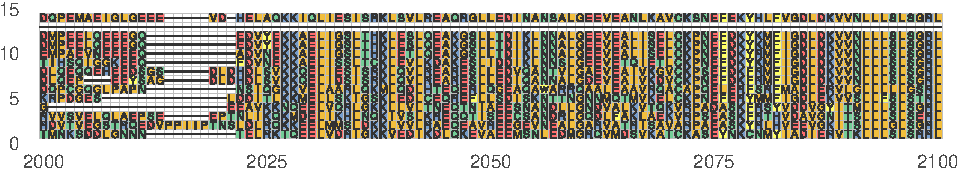
\includegraphics{lbrb_files/figure-latex/unnamed-chunk-157-1.pdf}

\hypertarget{saving-an-msa-as-pdf}{%
\subsubsection{Saving an MSA as PDF}\label{saving-an-msa-as-pdf}}

We can take a look at the alignment in PDF format if we want. I this case I'm going to just show about 100 amino acids near the end of the alignment, where there is the most overlap across all of the sequences. This is set with the \passthrough{\lstinline!y = c(...)!} argument.

\begin{lstlisting}[language=R]
msaPrettyPrint(shrooms_align,             # alignment
               file = "shroom_msa.pdf",   # file name
               y=c(2000, 2100),           # range
               askForOverwrite=FALSE)
\end{lstlisting}

You can see where R is saving things by running \passthrough{\lstinline!getwd()!}

\begin{lstlisting}[language=R]
getwd()
\end{lstlisting}

\begin{lstlisting}
## [1] "/Users/nlb24/OneDrive - University of Pittsburgh/0-books/lbrb-bk/lbrb"
\end{lstlisting}

On a Mac you can usually find the file by searching in Finder for the file name, which I set to be ``shroom\_msa.pdf'' using the \passthrough{\lstinline!file = ...!} argument above.

\hypertarget{genetic-distance.}{%
\section{Genetic distance.}\label{genetic-distance.}}

Next need to first get an estimate of how similar each sequences is. The more amino acids that are identical to each other, the more similar.

Instead of similarity, we usually work in terms of \emph{difference} or \textbf{genetic distance} (a.k.a. \textbf{evolutionary distance}). This is done with the \passthrough{\lstinline!dist.alignment()!} function.

\begin{lstlisting}[language=R]
shrooms_dist <- seqinr::dist.alignment(shrooms_align_seqinr, 
                                       matrix = "identity")
\end{lstlisting}

We've made a matrix using \passthrough{\lstinline!dist.alignment()!}; let's round it off so its easier to look at using the \passthrough{\lstinline!round()!} function.

\begin{lstlisting}[language=R]
shrooms_dist_rounded <- round(shrooms_dist,
                              digits = 3)
\end{lstlisting}

Now let's look at it

\begin{lstlisting}[language=R]
shrooms_dist_rounded
\end{lstlisting}

\begin{lstlisting}
##           NP_065768 AAK95579 AAF13269 AAF13270 NP_065910 ABD59319 CAA58534
## AAK95579      0.000                                                       
## AAF13269      0.884    0.917                                              
## AAF13270      0.897    0.917    0.000                                     
## NP_065910     0.878    0.912    0.533    0.536                            
## ABD59319      0.893    0.921    0.783    0.783     0.782                  
## CAA58534      0.872    0.908    0.838    0.849     0.840    0.864         
## ABD19518      0.866    0.912    0.834    0.846     0.838    0.855    0.548
## NP_597713     0.916    0.939    0.903    0.903     0.902    0.904    0.896
## CAA78718      0.925    0.955    0.896    0.895     0.893    0.893    0.898
## EAA12598      0.914    0.947    0.899    0.899     0.902    0.897    0.891
## ABA81834      0.938    0.943    0.935    0.934     0.936    0.940    0.935
## XP_392427     0.936    0.963    0.935    0.934     0.938    0.941    0.938
## XP_783573     0.940    0.958    0.942    0.939     0.942    0.935    0.942
##           ABD19518 NP_597713 CAA78718 EAA12598 ABA81834 XP_392427
## AAK95579                                                         
## AAF13269                                                         
## AAF13270                                                         
## NP_065910                                                        
## ABD59319                                                         
## CAA58534                                                         
## ABD19518                                                         
## NP_597713    0.900                                               
## CAA78718     0.891     0.919                                     
## EAA12598     0.896     0.920    0.922                            
## ABA81834     0.935     0.932    0.946    0.882                   
## XP_392427    0.934     0.927    0.947    0.878    0.923          
## XP_783573    0.946     0.947    0.941    0.925    0.954     0.943
\end{lstlisting}

\hypertarget{phylognetic-trees-finally}{%
\section{Phylognetic trees (finally!)}\label{phylognetic-trees-finally}}

We got our sequence, built multiple sequence alignment, and calculated the genetic distance between sequences. Now we are - finally - ready to build a phylogenetic tree.

First, we let R figure out the structure of the tree. There are \textbf{MANY} ways to build phylogenetic trees. We'll use a common one used for exploring sequences called \textbf{neighbor joining} algorithm via the function \passthrough{\lstinline!nj()!}. Neighbor joining uses genetic distances to cluster sequences into \textbf{clades}.

\begin{lstlisting}[language=R]
tree <- nj(shrooms_dist)
\end{lstlisting}

\hypertarget{plotting-phylogenetic-trees}{%
\subsection{Plotting phylogenetic trees}\label{plotting-phylogenetic-trees}}

Now we'll make a quick plot of our tree using \passthrough{\lstinline!plot()!} (and add a little label using a function called \passthrough{\lstinline!mtext()!}).

\begin{lstlisting}[language=R]
# plot tree
plot.phylo (tree, main="Phylogenetic Tree", 
            type = "unrooted", 
            use.edge.length = F)

# add label
mtext(text = "Shroom family gene tree - unrooted, no branch lengths")
\end{lstlisting}

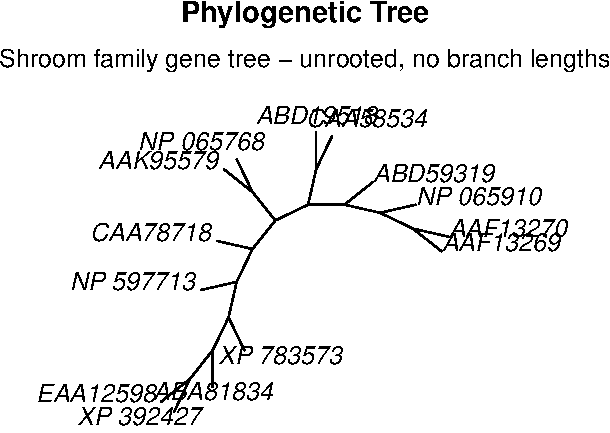
\includegraphics{lbrb_files/figure-latex/unnamed-chunk-164-1.pdf}

This is an **unrooted tree*. For the sake of plotting we've also ignored the evolutionary distance between the sequences.

To make a rooted tree we remove \passthrough{\lstinline!type = "unrooted!}.

\begin{lstlisting}[language=R]
# plot tree
plot.phylo (tree, main="Phylogenetic Tree", 
            use.edge.length = F)

# add label
mtext(text = "Shroom family gene tree - rooted, no branch lenths")
\end{lstlisting}

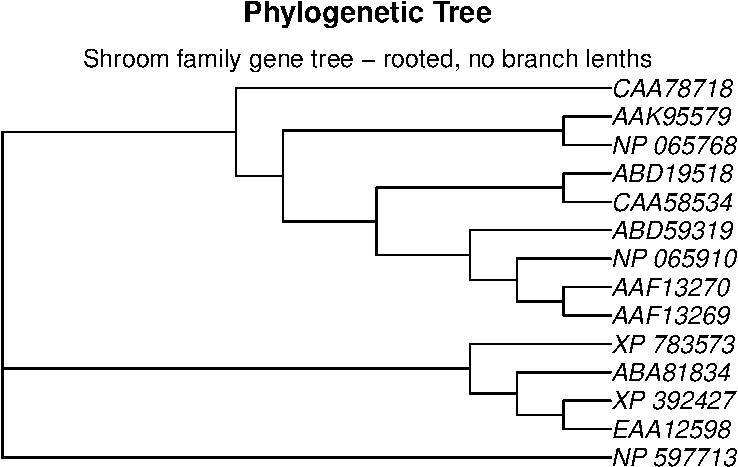
\includegraphics{lbrb_files/figure-latex/unnamed-chunk-165-1.pdf}

We can include information about branch length by setting \passthrough{\lstinline!use.edge.length = ...!} to \passthrough{\lstinline!T!}.

\begin{lstlisting}[language=R]
# plot tree
plot.phylo (tree, main="Phylogenetic Tree", 
            use.edge.length = T)

# add label
mtext(text = "Shroom family gene tree - rooted, with branch lenths")
\end{lstlisting}

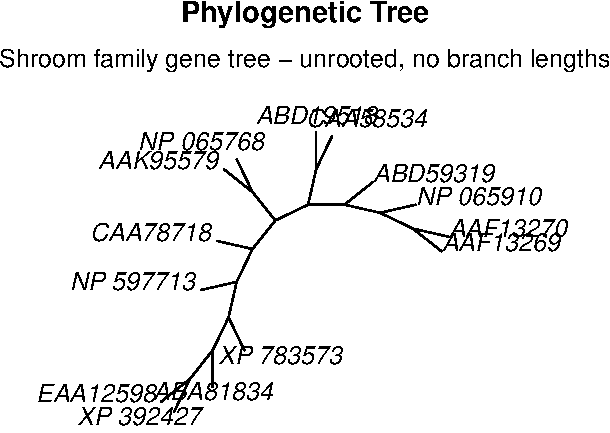
\includegraphics{lbrb_files/figure-latex/unnamed-chunk-166-1.pdf}

Some of the branches are now very short, but most are very long, indicating that these genes have been evolving independently for many millions of years.

Let's make a fancier plot. Don't worry about all the steps; I've added some more code to add some annotations on the right-hand side to help us see what's going on.

\begin{lstlisting}[language=R]
plot(tree, main="Phylogenetic Tree")
mtext(text = "Shroom family gene tree")

x <- 0.551
x2 <- 0.6

# label Shrm 3
segments(x0 = x, y0 = 1, 
         x1 = x, y1 = 4,
         lwd=2)
text(x = x*1.01, y = 2.5, "Shrm 3",adj = 0)

segments(x0 = x, y0 = 5, 
         x1 = x, y1 = 6,
         lwd=2)
text(x = x*1.01, y = 5.5, "Shrm 2",adj = 0)

segments(x0 = x, y0 = 7, 
         x1 = x, y1 = 9,
         lwd=2)
text(x = x*1.01, y = 8, "Shrm 1",adj = 0)

segments(x0 = x, y0 = 10, 
         x1 = x, y1 = 13,
         lwd=2)
text(x = x*1.01, y = 12, "Shrm ?",adj = 0)


segments(x0 = x, y0 = 14, 
         x1 = x, y1 = 15,
         lwd=2)
text(x = x*1.01, y = 14.5, "Shrm 4",adj = 0)


segments(x0 = x2, y0 = 1, 
         x1 = x2, y1 = 6,
         lwd=2)

segments(x0 = x2, y0 = 7, 
         x1 = x2, y1 = 9,
         lwd=2)

segments(x0 = x2, y0 = 10, 
         x1 = x2, y1 = 15,
         lwd=2)
\end{lstlisting}

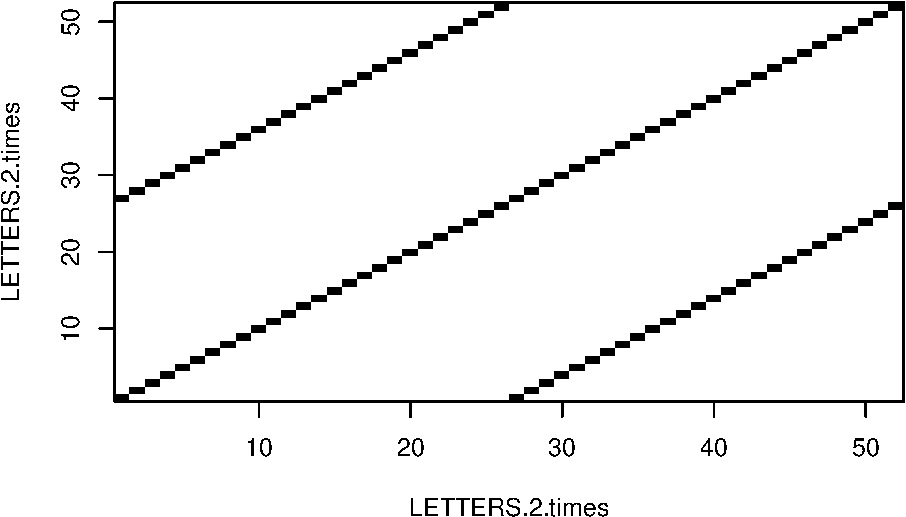
\includegraphics{lbrb_files/figure-latex/unnamed-chunk-167-1.pdf}

\hypertarget{logarithms-in-r}{%
\chapter{Logarithms in R}\label{logarithms-in-r}}

\textbf{By} Nathan Brouwer

Logging splits up multiplication into addition. So, log(m*n) is the same as log(m) + log(n)

You can check this

\begin{lstlisting}[language=R]
m<-10
n<-11
log(m*n)
\end{lstlisting}

\begin{lstlisting}
## [1] 4.70048
\end{lstlisting}

\begin{lstlisting}[language=R]
log(m)+log(n)
\end{lstlisting}

\begin{lstlisting}
## [1] 4.70048
\end{lstlisting}

\begin{lstlisting}[language=R]
log(m*n) == log(m)+log(n)
\end{lstlisting}

\begin{lstlisting}
## [1] TRUE
\end{lstlisting}

Exponentiation undos logs

\begin{lstlisting}[language=R]
exp(log(m*n))
\end{lstlisting}

\begin{lstlisting}
## [1] 110
\end{lstlisting}

\begin{lstlisting}[language=R]
m*n
\end{lstlisting}

\begin{lstlisting}
## [1] 110
\end{lstlisting}

The key equation in BLAST's E values is

u = ln(K\emph{m}n)/lambda

This can be changed to

{[}ln(K) + ln(mn){]}/lambda

We can check this

\begin{lstlisting}[language=R]
K <- 1
m <- 10
n <- 11
lambda <- 110

log(K*m*n)/lambda
\end{lstlisting}

\begin{lstlisting}
## [1] 0.04273164
\end{lstlisting}

\begin{lstlisting}[language=R]
(log(K) + log(m*n))/lambda
\end{lstlisting}

\begin{lstlisting}
## [1] 0.04273164
\end{lstlisting}

\begin{lstlisting}[language=R]
log(K*m*n)/lambda == (log(K) + log(m*n))/lambda
\end{lstlisting}

\begin{lstlisting}
## [1] TRUE
\end{lstlisting}

\hypertarget{part-appendices}{%
\part{Appendices}\label{part-appendices}}

\hypertarget{section}{%
\subsection*{}\label{section}}
\addcontentsline{toc}{subsection}{}

\hypertarget{appendix-01-getting-access-to-r}{%
\chapter*{Appendix 01: Getting access to R}\label{appendix-01-getting-access-to-r}}
\addcontentsline{toc}{chapter}{Appendix 01: Getting access to R}

\hypertarget{getting-started-with-r-and-rstudio}{%
\section{Getting Started With R and RStudio}\label{getting-started-with-r-and-rstudio}}

\begin{itemize}
\tightlist
\item
  R is a piece of software that does calculations and makes graphs.
\item
  RStudio is a GUI (graphical user interface) that acts as a front-end to R
\item
  Your can use R directly, but most people use a GUI of some kind
\item
  RStudio has become the most popular GUI
\end{itemize}

The following instructions will lead you click by click through downloading R and RStudio and starting an initial session. If you have trouble with downloading either program go to YouTube and search for something like ``Downloading R'' or ``Installing RStudio'' and you should be able to find something helpful, such as \href{https://www.youtube.com/watch?v=GYdmkLgV9n8}{``How to Download R for Windows''}.

\hypertarget{rstudio-cloud}{%
\subsection{RStudio Cloud}\label{rstudio-cloud}}

TODO: Add RStudio cloud

\hypertarget{getting-r-onto-your-own-computer}{%
\subsection{Getting R onto your own computer}\label{getting-r-onto-your-own-computer}}

To get R on to your computer first go to the \href{https://cran.r-project.org/}{CRAN website} at \url{https://cran.r-project.org/} (CRAN stands for ``comprehensive R Archive Network''). At the top of the screen are three bullet points; select the appropriate one (or click the link below)

\begin{itemize}
\tightlist
\item
  \href{https://cran.r-project.org/bin/linux/}{Download R for Linux}
\item
  \href{https://cran.r-project.org/bin/macosx/}{Download R for (Mac) OS X}
\item
  \href{https://cran.r-project.org/bin/windows/}{Download R for Windows}
\end{itemize}

Each page is formatted slightly differently. For a current Mac, click on the top link, which as of 8/16/2018 was ``\href{https://cran.r-project.org/bin/macosx/R-3.5.1.pkg}{R-3.5.1.pkg}'' or click this link. If you have an older Mac you might have to scroll down to find your operating system under ``Binaries for legacy OS X systems.''

For PC select ``\href{https://cran.r-project.org/bin/windows/base/}{base}'' or click this link.

When its downloaded, run the installer and accept the defaults.

\hypertarget{getting-rstudio-onto-your-computer}{%
\subsection{Getting RStudio onto your computer}\label{getting-rstudio-onto-your-computer}}

\href{www.rstudio.com/}{RStudio} is an R interface developed by a company of the same name. RStudio has a number of commercial products, but much of their portfolio is freeware. You can download RStudio from their website www.rstudio.com/ . The \href{https://www.rstudio.com/products/rstudio/download/}{download page} (www.rstudio.com/products/rstudio/download/) is a bit busy because it shows all of their commercial products; the free version is on the far left side of the table of products. Click on the big green DOWNLOAD button under the column on the left that says ``RStudio Desktop Open Source License'' (or click on this \href{https://www.rstudio.com/products/rstudio/download/\#download}{link} ).

This will scroll you down to a list of downloads titled ``Installers for Supported Platforms.'' Windows users can select the top option \href{https://download1.rstudio.org/RStudio-1.1.456.exe}{RStudio 1.1.456 - Windows Vista/7/8/10} and Mac the second option \href{https://download1.rstudio.org/RStudio-1.1.456.dmg}{RStudio 1.1.456 - Mac OS X 10.6+ (64-bit)}. (Versions names are current of 8/16/2018).

Run the installer after it downloads and accept the default. RStudio will automatically link up with the most current version of R you have on your computer. Find the RStudio icon on your desktop or search for ``RStudio'' from your task bar and you'll be read to go.

\hypertarget{keep-r-and-rstudio-current}{%
\subsection{Keep R and RStudio current}\label{keep-r-and-rstudio-current}}

Both R and RStudio undergo regular updates and you will occasionally have to re-download and install one or both of them. In practice I probably do this about every 6 months.

\hypertarget{getting-started-with-r-itself-or-not}{%
\chapter*{Getting started with R itself (or not)}\label{getting-started-with-r-itself-or-not}}
\addcontentsline{toc}{chapter}{Getting started with R itself (or not)}

\hypertarget{vocabulary-1}{%
\section*{Vocabulary}\label{vocabulary-1}}
\addcontentsline{toc}{section}{Vocabulary}

\begin{itemize}
\tightlist
\item
  console
\item
  script editor / source viewer
\item
  interactive programming
\item
  scripts / script files
\item
  .R files
\item
  text files / plain text files
\item
  command execution / execute a command from script editor
\item
  comments / code comments
\item
  commenting out / commenting out code
\item
  stackoverflow.com
\item
  the rstats hashtag
\end{itemize}

\hypertarget{r-commands}{%
\section*{R commands}\label{r-commands}}
\addcontentsline{toc}{section}{R commands}

\begin{itemize}
\tightlist
\item
  c(\ldots)
\item
  mean(\ldots)
\item
  sd(\ldots)
\item
  ?
\item
  read.csv(\ldots)
\end{itemize}

This is a walk-through of a very basic R session. It assumes you have successfully installed R and RStudio onto your computer, and nothing else.

Most people who use R do not actually use the program itself - they use a GUI (graphical user interface) ``front end'' that make R a bit easier to use. However, you will probably run into the icon for the underlying R program on your desktop or elsewhere on your computer. It usually looks like this:

ADD IMAGE HERE

The long string of numbers have to do with the version and whether is 32 or 64 bit (not important for what we do).

If you are curious you can open it up and take a look - it actually looks a lot like RStudio, where we will do all our work (or rather, RStudio looks like R). Sometimes when people are getting started with R they will accidentally open R instead of RStudio; if things don't seem to look or be working the way you think they should, you might be in R, not RStudio

\hypertarget{rs-console-as-a-scientific-calculator}{%
\subsubsection{R's console as a scientific calculator}\label{rs-console-as-a-scientific-calculator}}

You can interact with R's console similar to a scientific calculator. For example, you can use parentheses to set up mathematical statements like

\begin{lstlisting}[language=R]
5*(1+1)
\end{lstlisting}

\begin{lstlisting}
## [1] 10
\end{lstlisting}

Note however that you have to be explicit about multiplication. If you try the following it won't work.

\begin{lstlisting}[language=R]
5(1+1)
\end{lstlisting}

R also has built-in functions that work similar to what you might have used in Excel. For example, in Excel you can calculate the average of a set of numbers by typing ``=average(1,2,3)'' into a cell. R can do the same thing except

\begin{itemize}
\tightlist
\item
  The command is ``mean''
\item
  You don't start with ``=''
\item
  You have to package up the numbers like what is shown below using ``c(\ldots)''
\end{itemize}

\begin{lstlisting}[language=R]
mean(c(1,2,3))
\end{lstlisting}

\begin{lstlisting}
## [1] 2
\end{lstlisting}

Where ``c(\ldots)'' packages up the numbers the way the mean() function wants to see them.

If you just do the following R will give you an answer, but its the wrong one

\begin{lstlisting}[language=R]
mean(1,2,3)
\end{lstlisting}

\textbf{This is a common issue with R -- and many programs, really -- it won't always tell you when somethind didn't go as planned. This is because it doesn't know something didn't go as planned; you have to learn the rules R plays by.}

\hypertarget{practice-math-in-the-console}{%
\subsubsection{Practice: math in the console}\label{practice-math-in-the-console}}

See if you can reproduce the following results

\textbf{Division}

\begin{lstlisting}[language=R]
10/3
\end{lstlisting}

\begin{lstlisting}
## [1] 3.333333
\end{lstlisting}

\textbf{The standard deviation}

\begin{lstlisting}[language=R]
sd(c(5,10,15)) # note the use of "c(...)"
\end{lstlisting}

\begin{lstlisting}
## [1] 5
\end{lstlisting}

\hypertarget{the-script-editor}{%
\subsubsection{The script editor}\label{the-script-editor}}

While you can interact with R directly within the console, the standard way to work in R is to write what are known as \textbf{scripts.} These are computer code instructions written to R in a \textbf{script file.} These are save with the extension \textbf{.R} but area really just a form of \textbf{plain text file.}

To work with scripts, what you do is type commands in the script editor, then tell R to \textbf{excute} the command. This can be done several ways.

First, you tell RStudio the line of code you want to run by either
* Placing the cursor at the end a line of code, OR
* Clicking and dragging over the code you want to run in order highlight it.

Second, you tell RStudio to run the code by
* Clicking the ``Run'' icon in the upper right hand side of the script editor (a grey box with a green error emerging from it)
* pressing the control key (``ctrl)'' and then then enter key on the keyboard

The code you've chosen to run will be sent by RStudio from the script editor over to the console. The console will show you both the code and then the output.

You can run several lines of code if you want; the console will run a line, print the output, and then run the next line. First I'll use the command mean(), and then the command sd() for the standard deviation:

\begin{lstlisting}[language=R]
mean(c(1,2,3))
\end{lstlisting}

\begin{lstlisting}
## [1] 2
\end{lstlisting}

\begin{lstlisting}[language=R]
sd(c(1,2,3))
\end{lstlisting}

\begin{lstlisting}
## [1] 1
\end{lstlisting}

\hypertarget{comments}{%
\subsubsection{Comments}\label{comments}}

One of the reasons we use script files is that we can combine R code with \textbf{comments} that tell us what the R code is doing. Comments are preceded by the hashtag symbol \textbf{\#}. Frequently we'll write code like this:

\begin{lstlisting}[language=R]
#The mean of 3 numbers
mean(c(1,2,3))
\end{lstlisting}

If you highlight all of this code (including the comment) and then click on ``run'', you'll see that RStudio sends all of the code over console.

\begin{lstlisting}
## [1] 2
\end{lstlisting}

Comments can also be placed at the \emph{end} of a line of code

\begin{lstlisting}[language=R]
mean(c(1,2,3)) #Note  the use of c(...)
\end{lstlisting}

Sometimes we write code and then don't want R to run it. We can prevent R from executing the code even if its sent to the console by putting a ``\#'' \emph{infront} of the code.

If I run this code, I will get just the mean but not the sd.

\begin{lstlisting}[language=R]
mean(c(1,2,3))
#sd(c(1,2,3))
\end{lstlisting}

Doing this is called \textbf{commenting out} a line of code.

\hypertarget{help}{%
\section{Help!}\label{help}}

There are many resource for figuring out R and RStudio, including

\begin{itemize}
\tightlist
\item
  R's built in ``help'' function
\item
  Q\&A websites like \textbf{stackoverflow.com}
\item
  twitter, using the hashtag \#rstats
\item
  blogs
\item
  online books and course materials
\end{itemize}

\hypertarget{getting-help-from-r}{%
\subsection{Getting ``help'' from R}\label{getting-help-from-r}}

If you are using a function in R you can get info about how it works like this

\begin{lstlisting}[language=R]
?mean
\end{lstlisting}

In RStudio the help screen should appear, probably above your console. If you start reading this help file, though, you don't have to go far until you start seeing lots of R lingo, like ``S3 method'',``na.rm'', ``vectors''. Unfortunately, the R help files are usually not written for beginners, and reading help files is a skill you have to acquire.

For example, when we load data into R in subsequent lessons we will use a function called ``read.csv''

Access the help file by typing ``?read.csv'' into the console and pressing enter. Surprisingly, the function that R give you the help file isn't what you asked for, but is read.table(). This is a related function to read.csv, but when you're a beginner thing like this can really throw you off.

Kieran Healy as produced a great cheatsheet for reading R's help pages as part of his forthcoming book. It should be available online at \url{http://socviz.co/appendix.html\#a-little-more-about-r}

\hypertarget{getting-help-from-the-internet}{%
\subsection{Getting help from the internet}\label{getting-help-from-the-internet}}

The best way to get help for any topic is to just do an internet search like this: ``R read.csv''. Usually the first thing on the results list will be the R help file, but the second or third will be a blog post or something else where a usually helpful person has discussed how that function works.

Sometimes for very basic R commands like this might not always be productive but its always work a try. For but things related to stats, plotting, and programming there is frequently lots of information. Also try searching YouTube.

\hypertarget{getting-help-from-online-forums}{%
\subsection{Getting help from online forums}\label{getting-help-from-online-forums}}

Often when you do an internet search for an R topic you'll see results from the website www.stackoverflow.com, or maybe www.crossvalidated.com if its a statistics topic. These are excellent resources and many questions that you may have already have answers on them. Stackoverflow has an internal search function and also suggests potentially relevant posts.

Before posting to one of these sites yourself, however, do some research; there is a particular type and format of question that is most likely to get a useful response. Sadly, people new to the site often get ``flamed'' by impatient pros.

\hypertarget{getting-help-from-twitter}{%
\subsection{Getting help from twitter}\label{getting-help-from-twitter}}

Twitter is a surprisingly good place to get information or to find other people knew to R. Its often most useful to ask people for learning resources or general reference, but you can also post direct questions and see if anyone responds, though usually its more advanced users who engage in twitter-based code discussion.

A standard tweet might be
``Hey \#rstats twitter, am knew to \#rstats and really stuck on some of the basics. Any suggestions for good resources for someone starting from scratch?''

\hypertarget{other-features-of-rstudio}{%
\section{Other features of RStudio}\label{other-features-of-rstudio}}

\hypertarget{ajusting-pane-the-layout}{%
\subsection{Ajusting pane the layout}\label{ajusting-pane-the-layout}}

You can adjust the location of each of RStudio 4 window panes, as well as their size.

To set the pane layout go to
1. ''Tools'' on the top menu
1. ''Global options''
1. ``Pane Layout''

Use the drop-down menus to set things up. I recommend
1. Lower left: ``Console''''
1. Top right: ``Source''
1. Top left: ``Plot, Packages, Help Viewer''
1. This will leave the ``Environment\ldots{}'' panel in the lower right.

\hypertarget{adjusting-size-of-windows}{%
\subsection{Adjusting size of windows}\label{adjusting-size-of-windows}}

You can clicked on the edge of a pane and adjust its size. For most R work we want the console to be big. For beginners, the ``Environment, history, files'' panel can be made really small.

\hypertarget{practice-optional}{%
\section{Practice (OPTIONAL)}\label{practice-optional}}

Practice the following operations. Type the directly into the console and execute them. Also write them in a script in the script editor and run them.

\textbf{Square roots}

\begin{lstlisting}[language=R]
sqrt(42)
\end{lstlisting}

\begin{lstlisting}
## [1] 6.480741
\end{lstlisting}

\textbf{The date}
Some functions in R can be executed within nothing in the parentheses.

\begin{lstlisting}[language=R]
date()
\end{lstlisting}

\begin{lstlisting}
## [1] "Sat Sep 18 00:32:06 2021"
\end{lstlisting}

\textbf{Exponents}
The \textbf{\^{}} is used for exponents

\begin{lstlisting}[language=R]
42^2
\end{lstlisting}

\begin{lstlisting}
## [1] 1764
\end{lstlisting}

\textbf{A series of numbers}
A colon between two numbers creates a series of numbers.

\begin{lstlisting}[language=R]
1:42
\end{lstlisting}

\begin{lstlisting}
##  [1]  1  2  3  4  5  6  7  8  9 10 11 12 13 14 15 16 17 18 19 20 21 22 23 24 25
## [26] 26 27 28 29 30 31 32 33 34 35 36 37 38 39 40 41 42
\end{lstlisting}

\textbf{logs}
The default for the log() function is the natural log.

\begin{lstlisting}[language=R]
log(42)
\end{lstlisting}

\begin{lstlisting}
## [1] 3.73767
\end{lstlisting}

log10() gives the base-10 log.

\begin{lstlisting}[language=R]
log10(42)
\end{lstlisting}

\begin{lstlisting}
## [1] 1.623249
\end{lstlisting}

\textbf{exp() raises e to a power}

\begin{lstlisting}[language=R]
exp(3.73767)
\end{lstlisting}

\begin{lstlisting}
## [1] 42.00002
\end{lstlisting}

\textbf{Multiple commands can be nested}

\begin{lstlisting}[language=R]
sqrt(42)^2
log(sqrt(42)^2)
exp(log(sqrt(42)^2))
\end{lstlisting}

  \bibliography{book.bib,packages.bib}

\end{document}
